\documentclass[12pt]{article} 
\usepackage{amsmath,amsfonts,amssymb} 
\usepackage[usenames,dvipsnames]{xcolor} 
\usepackage{hyperref} 
\usepackage{fullpage} 
\usepackage{empheq} 
\usepackage{pgfplots} 
\usepackage{float}
\usepackage{color}
\usepackage{multirow}
\usepackage{algorithm} 
\usepackage{algorithmic}



\usetikzlibrary{external}
\tikzexternalize[prefix=paperOnImpFigures/,figure list=true] 

\begin{document}

\newcommand{\tr}{\mbox{tr}} 
\newtheorem{theorem}{Theorem}[section] 
\newtheorem{lemma}[theorem]{Lemma} 
\newtheorem{proposition}[theorem]{Proposition} 
\newtheorem{corollary}[theorem]{Corollary}

\pgfplotsset{compat=newest} 
\pgfplotsset{plot coordinates/math parser=false} 

\begin{titlepage}
	
	\hrule 
	\begin{center}
		\large \textsc{On the Implementation of Stochastic Quasi-Newton Methods}\\
	\end{center}
	\hrule \normalsize
	
	\bigskip 
	\bigskip
	
	\centering\today
	
	\bigskip 
	\bigskip
	
	\tableofcontents 
\end{titlepage}

\newpage

%%%%%%%%%%%%%%%%%%%%%%%%%%%%%%%%%%%%
\section{Small Batch Sizes Experiment}
\label{sec:aoverk}

\subsection{Parameters}
We compare the relative performance of sgd and sqn with small batch sizes. For both methods stepsize is $\frac{a}{k^p}$ 
\begin{itemize}
	\item b is the gradient batch size 
	\item a is the initial stepsize 
	\item p is the power of k 
	%\item PR is if doing Polyak-Ruppert averaging 
\end{itemize}

For sqn: 
\begin{itemize}
	\item L is periodicity of updating the QN matrix 
	\item M is the memory 
	\item bH is the hessian batch size 
\end{itemize}

\subsection{Work Computations}
We compute work in the following way:

For the sqn methods:
\begin{itemize}
	\item $b$ work per each iteration
	\item $bH$ work every $L$ iterations
	\item $4M$ work every iteration after the first hessian update happens
\end{itemize}

For the sgd methods:
\begin{itemize}
	\item $b$ work per each iteration 
\end{itemize}



\newpage

\subsection{Yoram's problem}

This is run for amount of work equivalent to SGD making 43 passes over the data. 

\begin{figure}[H]
% This file was created by matlab2tikz v0.4.6 running on MATLAB 8.2.
% Copyright (c) 2008--2014, Nico Schlömer <nico.schloemer@gmail.com>
% All rights reserved.
% Minimal pgfplots version: 1.3
% 
% The latest updates can be retrieved from
%   http://www.mathworks.com/matlabcentral/fileexchange/22022-matlab2tikz
% where you can also make suggestions and rate matlab2tikz.
% 
%
% defining custom colors
\definecolor{mycolor1}{rgb}{0.00000,1.00000,1.00000}%
%
\begin{tikzpicture}

\begin{axis}[%
width=6.02303149606299in,
height=4.75042322834646in,
scale only axis,
xmin=0,
xmax=300000,
xlabel={work},
ymode=log,
ymin=0.001,
ymax=10,
yminorticks=true,
ylabel={function values},
legend style={draw=black,fill=white,legend cell align=left}
]
\addplot [color=green,solid]
  table[row sep=crcr]{
1	1.81967985981371	\\
2	2.35903716011345	\\
4	2.12060646080914	\\
7	1.90505336162705	\\
14	1.85856569341987	\\
28	1.53310811293755	\\
54	1.36936832342705	\\
104	1.19171915574342	\\
202	0.968055308995	\\
393	0.841442497133661	\\
763	0.712745239529632	\\
1482	0.626884529541976	\\
2879	0.558289394659908	\\
5591	0.50161048827758	\\
10859	0.459234171507532	\\
21088	0.423021840105272	\\
40956	0.394293227905482	\\
79539	0.369371312992474	\\
154473	0.348922635288321	\\
300000	0.331121124761166	\\
};
\addlegendentry{ggb1a0.25p1PR0};

\addplot [color=red,solid]
  table[row sep=crcr]{
2	8.28798527167918	\\
4	7.18015191787079	\\
6	6.47119146121568	\\
8	6.45696148099933	\\
14	6.02849833139693	\\
28	4.964481026789	\\
54	3.46703479422194	\\
104	2.5245369102262	\\
202	1.75497129398163	\\
394	1.21746431775426	\\
764	0.857425029946482	\\
1482	0.666637962177253	\\
2880	0.506081064890632	\\
5592	0.419024631312934	\\
10860	0.355417570065038	\\
21088	0.306741131093211	\\
40956	0.270741404912369	\\
79540	0.242409313213422	\\
154474	0.220170220725227	\\
300000	0.20157255727814	\\
};
\addlegendentry{ggb2a1p1PR0};

\addplot [color=blue,solid]
  table[row sep=crcr]{
5	3.51833862930559	\\
10	2.72466541951842	\\
15	2.74572905907864	\\
20	2.77823853257425	\\
25	2.49154462581404	\\
30	2.49175500304373	\\
55	1.67403943787081	\\
105	1.21135009948362	\\
205	0.906636784638991	\\
395	0.69576184458046	\\
765	0.511522916759083	\\
1485	0.421284450039153	\\
2880	0.353004651231351	\\
5595	0.302402458520536	\\
10860	0.264658807967606	\\
21090	0.236069243895937	\\
40960	0.213426028963344	\\
79540	0.195011512627053	\\
154475	0.180669220277826	\\
300000	0.168834895348674	\\
};
\addlegendentry{ggb5a1p1PR0};

\addplot [color=black,solid]
  table[row sep=crcr]{
10	6.82578201598315	\\
20	8.34363918816818	\\
30	7.605558741688	\\
40	6.24165485788079	\\
50	5.24999171006859	\\
60	4.68490765775779	\\
70	4.46471917710477	\\
110	3.1649215135313	\\
210	2.26276174045294	\\
400	1.49742092502788	\\
770	0.926169006507993	\\
1490	0.67583896464119	\\
2880	0.510955761419618	\\
5600	0.378475956305734	\\
10860	0.295702867209854	\\
21090	0.235679163973348	\\
40960	0.194052652993265	\\
79540	0.162798118246854	\\
154480	0.140448629976203	\\
300000	0.123357901937189	\\
};
\addlegendentry{ggb10a4p1PR0};

\addplot [color=mycolor1,solid]
  table[row sep=crcr]{
50	7.97769524929225	\\
100	3.82539981136845	\\
150	2.71371185112556	\\
200	2.46218684309712	\\
250	1.85656386195242	\\
300	1.70686025650355	\\
350	1.49813690010845	\\
400	1.34741126854456	\\
450	1.2687611392708	\\
500	1.04969305317595	\\
800	0.737213159981588	\\
1500	0.485485962988792	\\
2900	0.300036069634242	\\
5600	0.214820857513687	\\
10900	0.168120140230615	\\
21100	0.135483780787145	\\
41000	0.114607411355743	\\
79550	0.0996038032022017	\\
154500	0.0881654502347509	\\
300000	0.0799275918672878	\\
};
\addlegendentry{ggb50a8p1PR0};

\addplot [color=green,solid,mark=asterisk,mark options={solid}]
  table[row sep=crcr]{
1	1.81967985981371	\\
2	2.35903716011345	\\
4	2.12060646080914	\\
7	1.90505336162705	\\
650	3.91444950191055	\\
691	3.73747653665743	\\
732	3.73747656004447	\\
773	4.04012463685925	\\
814	3.61447887087111	\\
855	2.97264088192215	\\
1660	2.81318813528088	\\
2670	1.24680735591811	\\
4690	0.687528846391381	\\
9740	0.560858020210105	\\
17820	0.502496301935344	\\
34990	0.4349229780559	\\
68320	0.378206959670374	\\
131950	0.333561794356932	\\
256180	0.304885027061974	\\
496560	0.278687516898935	\\
};
\addlegendentry{sqnb1a0.25p1L10M10bH600PR0};

\addplot [color=red,solid,mark=asterisk,mark options={solid}]
  table[row sep=crcr]{
2	4.2000039760198	\\
4	3.66020689346328	\\
6	3.30516143651586	\\
8	3.29414702372477	\\
14	3.08044231363236	\\
660	2.82595228104176	\\
702	2.8309945308166	\\
744	2.83227088032179	\\
786	2.96465218313476	\\
828	4.83817639514149	\\
1680	1.85829302167597	\\
2700	1.4580181518698	\\
4740	0.531778941373616	\\
9072	0.398772621656114	\\
18000	0.332499533123937	\\
34488	0.277578633852172	\\
67980	0.233785761674324	\\
131220	0.196495920032849	\\
254640	0.167047990301914	\\
493320	0.143610447579882	\\
};
\addlegendentry{sqnb2a0.5p1L10M10bH600PR0};

\addplot [color=blue,solid,mark=asterisk,mark options={solid}]
  table[row sep=crcr]{
5	1.86458820315441	\\
10	1.43764713167609	\\
15	1.43895979425734	\\
20	1.44952170400871	\\
25	1.32098179683445	\\
30	1.3230843696155	\\
690	0.927582199480627	\\
735	0.920085680759885	\\
780	1.04682441725188	\\
825	1.03156270197086	\\
1740	0.609081500402802	\\
2790	0.455696633066358	\\
4890	0.364340364590855	\\
9090	0.309258893865294	\\
17490	0.257237566203099	\\
34290	0.211314627438863	\\
65880	0.172915013005035	\\
128790	0.140870682110729	\\
249540	0.11690576597111	\\
484740	0.0973974628282433	\\
};
\addlegendentry{sqnb5a0.5p1L10M10bH600PR0};

\addplot [color=black,solid,mark=asterisk,mark options={solid}]
  table[row sep=crcr]{
10	1.80275476759502	\\
20	2.16366504503441	\\
30	1.98854714820968	\\
40	1.60554628888675	\\
50	1.32696512384994	\\
60	1.1760507257066	\\
70	1.1299384681061	\\
740	0.987235003297552	\\
790	2.45663124435007	\\
840	2.54928858212473	\\
1090	1.30714262569744	\\
2290	0.567779115997088	\\
4440	0.189201836804934	\\
8440	0.157031385558008	\\
17240	0.124234439030448	\\
33090	0.0981204330543716	\\
64540	0.074613725830218	\\
125040	0.0532531827329113	\\
242740	0.0385811875278652	\\
471540	0.0302333197242199	\\
};
\addlegendentry{sqnb10a1p1L10M10bH600PR0};

\addplot [color=mycolor1,solid,mark=asterisk,mark options={solid}]
  table[row sep=crcr]{
50	2.05605381548433	\\
100	1.01813310471464	\\
150	0.720517699211241	\\
200	0.649168719019453	\\
250	0.502611581447363	\\
300	0.467211837176879	\\
350	0.424593823981775	\\
400	0.3952651858322	\\
450	0.374318791078798	\\
1140	1.2916674067754	\\
1230	1.33724985557563	\\
1860	0.277174919380206	\\
4140	0.138418224281027	\\
7320	0.0991111681595106	\\
14640	0.062935628893658	\\
28500	0.0423189725035129	\\
55680	0.0260977442552728	\\
108270	0.0187254134411956	\\
211140	0.016024206173695	\\
409140	0.012097098648358	\\
};
\addlegendentry{sqnb50a2p1L10M10bH600PR0};

\end{axis}
\end{tikzpicture}%
\caption{Test Function Value}
\end{figure}

\begin{figure}[H]
% This file was created by matlab2tikz v0.4.6 running on MATLAB 8.2.
% Copyright (c) 2008--2014, Nico Schlömer <nico.schloemer@gmail.com>
% All rights reserved.
% Minimal pgfplots version: 1.3
% 
% The latest updates can be retrieved from
%   http://www.mathworks.com/matlabcentral/fileexchange/22022-matlab2tikz
% where you can also make suggestions and rate matlab2tikz.
% 
%
% defining custom colors
\definecolor{mycolor1}{rgb}{0.00000,1.00000,1.00000}%
%
\begin{tikzpicture}

\begin{axis}[%
width=6.02303149606299in,
height=4.75042322834646in,
scale only axis,
xmin=0,
xmax=300000,
xlabel={iterations},
ymode=log,
ymin=0.001,
ymax=10,
yminorticks=true,
ylabel={function values},
legend style={draw=black,fill=white,legend cell align=left}
]
\addplot [color=green,solid]
  table[row sep=crcr]{
1	1.81856350996846	\\
2	2.2875304277347	\\
4	2.05924649410991	\\
7	1.83292861531095	\\
14	1.81286464712082	\\
28	1.46599726562721	\\
54	1.29761519832183	\\
104	1.12562840980094	\\
202	0.913234689589722	\\
393	0.791384438866444	\\
763	0.672662437017766	\\
1482	0.590386983329786	\\
2879	0.524849862227999	\\
5591	0.47104194878916	\\
10859	0.431030336180643	\\
21088	0.397605769679248	\\
40956	0.37079300493578	\\
79539	0.347690786339436	\\
154473	0.328787179011531	\\
300000	0.312308377491829	\\
};
\addlegendentry{ggb1a0.25p1PR0};

\addplot [color=red,solid]
  table[row sep=crcr]{
1	8.0381962692073	\\
2	7.00192112660946	\\
3	6.42655683714102	\\
4	6.41305381793496	\\
7	6.01470756127528	\\
14	4.84421100042688	\\
27	3.36463328759554	\\
52	2.4524612359178	\\
101	1.71792635333949	\\
197	1.19269195132663	\\
382	0.840941303058544	\\
741	0.648154051959699	\\
1440	0.490691883967582	\\
2796	0.404240537443014	\\
5430	0.341827671033895	\\
10544	0.294585281332411	\\
20478	0.260095115970006	\\
39770	0.233102240113561	\\
77237	0.211948304995436	\\
150000	0.19430657896511	\\
};
\addlegendentry{ggb2a1p1PR0};

\addplot [color=blue,solid]
  table[row sep=crcr]{
1	3.3386108072812	\\
2	2.55420047969045	\\
3	2.62778710438479	\\
4	2.65722130486094	\\
5	2.33504695099728	\\
6	2.33543662824613	\\
11	1.5279043563248	\\
21	1.09309843022196	\\
41	0.818457517027273	\\
79	0.624094620029965	\\
153	0.458487087542229	\\
297	0.377860466540215	\\
576	0.318348722699485	\\
1119	0.273416776980247	\\
2172	0.239833589342966	\\
4218	0.214835546618593	\\
8192	0.195393481240517	\\
15908	0.179594658325053	\\
30895	0.167273223815419	\\
60000	0.157217158464251	\\
};
\addlegendentry{ggb5a1p1PR0};

\addplot [color=black,solid]
  table[row sep=crcr]{
1	6.28246422336021	\\
2	7.86923134147495	\\
3	7.01726341806683	\\
4	5.87599960255149	\\
5	4.95502138718453	\\
6	4.47003891970361	\\
7	4.28484389342044	\\
11	3.02153327614434	\\
21	2.15366088953579	\\
40	1.45351420848693	\\
77	0.907906743146545	\\
149	0.650537662811193	\\
288	0.487552028907282	\\
560	0.361041436597042	\\
1086	0.280591847566324	\\
2109	0.223722941427258	\\
4096	0.184188173250957	\\
7954	0.153864263983221	\\
15448	0.13161781529604	\\
30000	0.114815187546449	\\
};
\addlegendentry{ggb10a4p1PR0};

\addplot [color=mycolor1,solid]
  table[row sep=crcr]{
1	7.5074512858424	\\
2	3.54774368672921	\\
3	2.55275189307841	\\
4	2.35921371551473	\\
5	1.79361747768468	\\
6	1.63618360250333	\\
7	1.44844016021952	\\
8	1.30062029445754	\\
9	1.22609920382895	\\
10	1.01081427623562	\\
16	0.748617742024943	\\
30	0.502067873397064	\\
58	0.309415980327582	\\
112	0.219936044148202	\\
218	0.167512993281501	\\
422	0.132480899288292	\\
820	0.109429900488735	\\
1591	0.0928490403490198	\\
3090	0.081035089765929	\\
6000	0.072306520143944	\\
};
\addlegendentry{ggb50a8p1PR0};

\addplot [color=green,solid,mark=asterisk,mark options={solid}]
  table[row sep=crcr]{
1	1.81856350996846	\\
2	2.2875304277347	\\
4	2.05924649410991	\\
7	1.83292861531095	\\
10	3.87724269615318	\\
11	3.64238766239739	\\
12	3.64238768435718	\\
13	3.90671992568409	\\
14	3.68277794551325	\\
15	3.00947450344089	\\
20	2.97263286461665	\\
30	1.38952100338493	\\
50	0.747810535361818	\\
100	0.604928860849352	\\
180	0.543963894158477	\\
350	0.467177563605428	\\
680	0.404082902968637	\\
1310	0.351861607807157	\\
2540	0.318478882275677	\\
4920	0.288958248547578	\\
};
\addlegendentry{sqnb1a0.25p1L10M10bH600PR0};

\addplot [color=red,solid,mark=asterisk,mark options={solid}]
  table[row sep=crcr]{
1	4.07700041428607	\\
2	3.56726651729082	\\
3	3.27711314967997	\\
4	3.26709263405805	\\
7	3.06454990580171	\\
10	2.77619867435884	\\
11	2.85187895709394	\\
12	2.85087053598223	\\
13	2.94102785299243	\\
14	4.82042926632597	\\
20	1.96087009983836	\\
30	1.49557887957549	\\
50	0.543085643016862	\\
96	0.399518330625702	\\
180	0.330214423895539	\\
344	0.275284159070588	\\
670	0.232503439485715	\\
1290	0.195753102323381	\\
2500	0.166526020358194	\\
4840	0.143346687819155	\\
};
\addlegendentry{sqnb2a0.5p1L10M10bH600PR0};

\addplot [color=blue,solid,mark=asterisk,mark options={solid}]
  table[row sep=crcr]{
1	1.77540499537238	\\
2	1.35159311009866	\\
3	1.37306919308655	\\
4	1.3776751448374	\\
5	1.22991606887111	\\
6	1.23579487512883	\\
10	0.838699659268413	\\
11	0.82178129898758	\\
12	1.02225138295043	\\
13	1.03771290079498	\\
20	0.621630033373084	\\
30	0.463690093608783	\\
50	0.361787160182776	\\
90	0.304770398613237	\\
170	0.25038938205624	\\
330	0.205452492854445	\\
632	0.168826608127395	\\
1230	0.138324417529698	\\
2380	0.115453203489747	\\
4620	0.0966627261511035	\\
};
\addlegendentry{sqnb5a0.5p1L10M10bH600PR0};

\addplot [color=black,solid,mark=asterisk,mark options={solid}]
  table[row sep=crcr]{
1	1.66550622499846	\\
2	2.05085279470099	\\
3	1.84924804678441	\\
4	1.51219249704062	\\
5	1.24752671695832	\\
6	1.11752788092715	\\
7	1.07686038919981	\\
10	0.968771899440981	\\
11	2.48468680206028	\\
12	2.57258214535798	\\
17	1.4086432365163	\\
29	0.590169669696801	\\
48	0.198843393947772	\\
80	0.165121306724716	\\
160	0.125291808539788	\\
309	0.0984933960038006	\\
590	0.0751662528305643	\\
1140	0.053754454168606	\\
2210	0.0390637226150403	\\
4290	0.0288435267731781	\\
};
\addlegendentry{sqnb10a1p1L10M10bH600PR0};

\addplot [color=mycolor1,solid,mark=asterisk,mark options={solid}]
  table[row sep=crcr]{
1	1.93764212580612	\\
2	0.949707351491012	\\
3	0.685230339797425	\\
4	0.624626559487793	\\
5	0.487678871858719	\\
6	0.448933295456803	\\
7	0.41178877446343	\\
8	0.382205871611635	\\
9	0.362799200265218	\\
10	1.27030323153458	\\
11	1.31789404505742	\\
18	0.261545511434571	\\
30	0.131658376510705	\\
52	0.0928836862298226	\\
100	0.0582080642338867	\\
194	0.0388114743879756	\\
376	0.0246882808625415	\\
727	0.0159319087368125	\\
1410	0.0118872658233016	\\
2730	0.00751975115184459	\\
};
\addlegendentry{sqnb50a2p1L10M10bH600PR0};

\end{axis}
\end{tikzpicture}%
\caption{Test Function Value}
\end{figure}
\begin{figure}[H]
% This file was created by matlab2tikz v0.4.6 running on MATLAB 8.2.
% Copyright (c) 2008--2014, Nico Schlömer <nico.schloemer@gmail.com>
% All rights reserved.
% Minimal pgfplots version: 1.3
% 
% The latest updates can be retrieved from
%   http://www.mathworks.com/matlabcentral/fileexchange/22022-matlab2tikz
% where you can also make suggestions and rate matlab2tikz.
% 
%
% defining custom colors
\definecolor{mycolor1}{rgb}{0.00000,1.00000,1.00000}%
%
\begin{tikzpicture}

\begin{axis}[%
width=6.02303149606299in,
height=4.75042322834646in,
scale only axis,
xmode=log,
xmin=0,
xmax=300000,
xminorticks=true,
xlabel={iterations},
ymode=log,
ymin=0.001,
ymax=10,
yminorticks=true,
ylabel={function values},
legend style={draw=black,fill=white,legend cell align=left}
]
\addplot [color=green,solid]
  table[row sep=crcr]{
1	1.81856350996846	\\
2	2.2875304277347	\\
4	2.05924649410991	\\
7	1.83292861531095	\\
14	1.81286464712082	\\
28	1.46599726562721	\\
54	1.29761519832183	\\
104	1.12562840980094	\\
202	0.913234689589722	\\
393	0.791384438866444	\\
763	0.672662437017766	\\
1482	0.590386983329786	\\
2879	0.524849862227999	\\
5591	0.47104194878916	\\
10859	0.431030336180643	\\
21088	0.397605769679248	\\
40956	0.37079300493578	\\
79539	0.347690786339436	\\
154473	0.328787179011531	\\
300000	0.312308377491829	\\
};
\addlegendentry{ggb1a0.25p1PR0};

\addplot [color=red,solid]
  table[row sep=crcr]{
1	8.0381962692073	\\
2	7.00192112660946	\\
3	6.42655683714102	\\
4	6.41305381793496	\\
7	6.01470756127528	\\
14	4.84421100042688	\\
27	3.36463328759554	\\
52	2.4524612359178	\\
101	1.71792635333949	\\
197	1.19269195132663	\\
382	0.840941303058544	\\
741	0.648154051959699	\\
1440	0.490691883967582	\\
2796	0.404240537443014	\\
5430	0.341827671033895	\\
10544	0.294585281332411	\\
20478	0.260095115970006	\\
39770	0.233102240113561	\\
77237	0.211948304995436	\\
150000	0.19430657896511	\\
};
\addlegendentry{ggb2a1p1PR0};

\addplot [color=blue,solid]
  table[row sep=crcr]{
1	3.3386108072812	\\
2	2.55420047969045	\\
3	2.62778710438479	\\
4	2.65722130486094	\\
5	2.33504695099728	\\
6	2.33543662824613	\\
11	1.5279043563248	\\
21	1.09309843022196	\\
41	0.818457517027273	\\
79	0.624094620029965	\\
153	0.458487087542229	\\
297	0.377860466540215	\\
576	0.318348722699485	\\
1119	0.273416776980247	\\
2172	0.239833589342966	\\
4218	0.214835546618593	\\
8192	0.195393481240517	\\
15908	0.179594658325053	\\
30895	0.167273223815419	\\
60000	0.157217158464251	\\
};
\addlegendentry{ggb5a1p1PR0};

\addplot [color=black,solid]
  table[row sep=crcr]{
1	6.28246422336021	\\
2	7.86923134147495	\\
3	7.01726341806683	\\
4	5.87599960255149	\\
5	4.95502138718453	\\
6	4.47003891970361	\\
7	4.28484389342044	\\
11	3.02153327614434	\\
21	2.15366088953579	\\
40	1.45351420848693	\\
77	0.907906743146545	\\
149	0.650537662811193	\\
288	0.487552028907282	\\
560	0.361041436597042	\\
1086	0.280591847566324	\\
2109	0.223722941427258	\\
4096	0.184188173250957	\\
7954	0.153864263983221	\\
15448	0.13161781529604	\\
30000	0.114815187546449	\\
};
\addlegendentry{ggb10a4p1PR0};

\addplot [color=mycolor1,solid]
  table[row sep=crcr]{
1	7.5074512858424	\\
2	3.54774368672921	\\
3	2.55275189307841	\\
4	2.35921371551473	\\
5	1.79361747768468	\\
6	1.63618360250333	\\
7	1.44844016021952	\\
8	1.30062029445754	\\
9	1.22609920382895	\\
10	1.01081427623562	\\
16	0.748617742024943	\\
30	0.502067873397064	\\
58	0.309415980327582	\\
112	0.219936044148202	\\
218	0.167512993281501	\\
422	0.132480899288292	\\
820	0.109429900488735	\\
1591	0.0928490403490198	\\
3090	0.081035089765929	\\
6000	0.072306520143944	\\
};
\addlegendentry{ggb50a8p1PR0};

\addplot [color=green,solid,mark=asterisk,mark options={solid}]
  table[row sep=crcr]{
1	1.81856350996846	\\
2	2.2875304277347	\\
4	2.05924649410991	\\
7	1.83292861531095	\\
10	3.87724269615318	\\
11	3.64238766239739	\\
12	3.64238768435718	\\
13	3.90671992568409	\\
14	3.68277794551325	\\
15	3.00947450344089	\\
20	2.97263286461665	\\
30	1.38952100338493	\\
50	0.747810535361818	\\
100	0.604928860849352	\\
180	0.543963894158477	\\
350	0.467177563605428	\\
680	0.404082902968637	\\
1310	0.351861607807157	\\
2540	0.318478882275677	\\
4920	0.288958248547578	\\
};
\addlegendentry{sqnb1a0.25p1L10M10bH600PR0};

\addplot [color=red,solid,mark=asterisk,mark options={solid}]
  table[row sep=crcr]{
1	4.07700041428607	\\
2	3.56726651729082	\\
3	3.27711314967997	\\
4	3.26709263405805	\\
7	3.06454990580171	\\
10	2.77619867435884	\\
11	2.85187895709394	\\
12	2.85087053598223	\\
13	2.94102785299243	\\
14	4.82042926632597	\\
20	1.96087009983836	\\
30	1.49557887957549	\\
50	0.543085643016862	\\
96	0.399518330625702	\\
180	0.330214423895539	\\
344	0.275284159070588	\\
670	0.232503439485715	\\
1290	0.195753102323381	\\
2500	0.166526020358194	\\
4840	0.143346687819155	\\
};
\addlegendentry{sqnb2a0.5p1L10M10bH600PR0};

\addplot [color=blue,solid,mark=asterisk,mark options={solid}]
  table[row sep=crcr]{
1	1.77540499537238	\\
2	1.35159311009866	\\
3	1.37306919308655	\\
4	1.3776751448374	\\
5	1.22991606887111	\\
6	1.23579487512883	\\
10	0.838699659268413	\\
11	0.82178129898758	\\
12	1.02225138295043	\\
13	1.03771290079498	\\
20	0.621630033373084	\\
30	0.463690093608783	\\
50	0.361787160182776	\\
90	0.304770398613237	\\
170	0.25038938205624	\\
330	0.205452492854445	\\
632	0.168826608127395	\\
1230	0.138324417529698	\\
2380	0.115453203489747	\\
4620	0.0966627261511035	\\
};
\addlegendentry{sqnb5a0.5p1L10M10bH600PR0};

\addplot [color=black,solid,mark=asterisk,mark options={solid}]
  table[row sep=crcr]{
1	1.66550622499846	\\
2	2.05085279470099	\\
3	1.84924804678441	\\
4	1.51219249704062	\\
5	1.24752671695832	\\
6	1.11752788092715	\\
7	1.07686038919981	\\
10	0.968771899440981	\\
11	2.48468680206028	\\
12	2.57258214535798	\\
17	1.4086432365163	\\
29	0.590169669696801	\\
48	0.198843393947772	\\
80	0.165121306724716	\\
160	0.125291808539788	\\
309	0.0984933960038006	\\
590	0.0751662528305643	\\
1140	0.053754454168606	\\
2210	0.0390637226150403	\\
4290	0.0288435267731781	\\
};
\addlegendentry{sqnb10a1p1L10M10bH600PR0};

\addplot [color=mycolor1,solid,mark=asterisk,mark options={solid}]
  table[row sep=crcr]{
1	1.93764212580612	\\
2	0.949707351491012	\\
3	0.685230339797425	\\
4	0.624626559487793	\\
5	0.487678871858719	\\
6	0.448933295456803	\\
7	0.41178877446343	\\
8	0.382205871611635	\\
9	0.362799200265218	\\
10	1.27030323153458	\\
11	1.31789404505742	\\
18	0.261545511434571	\\
30	0.131658376510705	\\
52	0.0928836862298226	\\
100	0.0582080642338867	\\
194	0.0388114743879756	\\
376	0.0246882808625415	\\
727	0.0159319087368125	\\
1410	0.0118872658233016	\\
2730	0.00751975115184459	\\
};
\addlegendentry{sqnb50a2p1L10M10bH600PR0};

\end{axis}
\end{tikzpicture}%
\caption{Test Function Value}
\end{figure}
Initially sgd methods achieve better test function values, but after many passes over the data, the sqn methods start improving upon the sgd methods, in terms of work needed to reach good generalization errors. This is true for all batch sizes. It is not clear if we found the best possible batch size for either method, since the highest we tried, 50, seemed to be the best. 
\newpage

\subsection{Speech problem}
This is run for amount of work equivalent to SGD making five passes over the data.

\begin{figure}[H]
% This file was created by matlab2tikz v0.4.6 running on MATLAB 8.2.
% Copyright (c) 2008--2014, Nico Schlömer <nico.schloemer@gmail.com>
% All rights reserved.
% Minimal pgfplots version: 1.3
% 
% The latest updates can be retrieved from
%   http://www.mathworks.com/matlabcentral/fileexchange/22022-matlab2tikz
% where you can also make suggestions and rate matlab2tikz.
% 
%
% defining custom colors
\definecolor{mycolor1}{rgb}{0.00000,1.00000,1.00000}%
%
\begin{tikzpicture}

\begin{axis}[%
width=6.02303149606299in,
height=4.75042322834646in,
unbounded coords=jump,
scale only axis,
xmin=0,
xmax=718530,
xlabel={work},
ymode=log,
ymin=1.58489319246111,
ymax=3.98107170553497,
yminorticks=true,
ylabel={function values},
legend style={draw=black,fill=white,legend cell align=left}
]
\addplot [color=green,solid]
  table[row sep=crcr]{
1	7.73932825640361	\\
2	7.85483869011965	\\
4	7.65008688435836	\\
8	7.99694683183218	\\
17	6.76034653985052	\\
35	5.47603379321278	\\
71	4.89256009209733	\\
144	4.52060953440647	\\
292	4.33486492321432	\\
594	4.16172687303218	\\
1209	4.00854810046246	\\
2458	3.86991070655154	\\
4998	3.75746986276036	\\
10163	3.65932974599413	\\
20667	3.57304870546916	\\
42025	3.49874668777833	\\
85456	3.43152604940314	\\
173771	3.37376352878611	\\
353355	3.32227038899969	\\
718530	3.27531518770878	\\
};
\addlegendentry{ggb1a0.5p1PR0};

\addplot [color=red,solid]
  table[row sep=crcr]{
2	7.48989498758627	\\
4	7.23261245065289	\\
6	7.46982204106989	\\
8	7.4077911448539	\\
18	6.38598711285454	\\
36	5.79390087438709	\\
72	5.45968029761965	\\
144	5.1033339856493	\\
292	4.80052599493207	\\
594	4.52132771086373	\\
1210	4.30622086591469	\\
2458	4.07814712059131	\\
4998	3.91228115282529	\\
10164	3.76688350836593	\\
20668	3.64546455869089	\\
42026	3.54059650665133	\\
85456	3.45196876418689	\\
173772	3.3758103558491	\\
353356	3.30979483233934	\\
718530	3.25230332517535	\\
};
\addlegendentry{ggb2a0.5p1PR0};

\addplot [color=blue,solid]
  table[row sep=crcr]{
5	7.58706692056241	\\
10	7.16214339178192	\\
15	6.8557394899359	\\
20	6.62565963923261	\\
25	6.04100118440144	\\
35	5.47842711520325	\\
75	4.93575198578481	\\
145	4.61880070809279	\\
295	4.3135262499356	\\
595	4.03967578854919	\\
1210	3.81080969747271	\\
2460	3.59515360091899	\\
5000	3.45358998354787	\\
10165	3.32843248443481	\\
20670	3.23101026016059	\\
42025	3.14757101591913	\\
85460	3.07604468592332	\\
173775	3.01328245620099	\\
353355	2.95753342288578	\\
718530	2.90728867152169	\\
};
\addlegendentry{ggb5a1p1PR0};

\addplot [color=black,solid]
  table[row sep=crcr]{
10	11.0761463770652	\\
20	11.384663436414	\\
30	10.3465113701884	\\
40	9.48163119008288	\\
50	9.07172598520908	\\
60	8.85961628822844	\\
80	8.33207089487304	\\
150	7.04186592978744	\\
300	5.74553031080812	\\
600	4.65298054615489	\\
1210	4.22131333528625	\\
2460	3.85249133695971	\\
5000	3.59436411866789	\\
10170	3.39428356831075	\\
20670	3.23710275588581	\\
42030	3.11068931311757	\\
85460	3.00082737258259	\\
173780	2.9069333627708	\\
353360	2.82616805796111	\\
718530	2.75497614286075	\\
};
\addlegendentry{ggb10a2p1PR0};

\addplot [color=mycolor1,solid]
  table[row sep=crcr]{
50	16.9969052113362	\\
100	13.8366764865375	\\
150	12.2376284955991	\\
200	10.0225130684837	\\
250	9.29705606189802	\\
300	8.38030472175263	\\
350	7.85915906116819	\\
400	7.32809881678845	\\
450	7.04031226026176	\\
600	6.41798690037746	\\
1250	4.89588011298422	\\
2500	4.01819112634152	\\
5000	3.40290487684742	\\
10200	2.99280760537857	\\
20700	2.72333193351891	\\
42050	2.53937511655976	\\
85500	2.40564186788351	\\
173800	2.31000431735197	\\
353400	2.23893963907787	\\
718550	2.18422462285574	\\
};
\addlegendentry{ggb50a8p1PR0};

\addplot [color=green,solid,mark=asterisk,mark options={solid}]
  table[row sep=crcr]{
1	12.493648364121	\\
2	13.2822598512112	\\
4	12.7930712043957	\\
8	14.3207162820109	\\
17	11.7576657509862	\\
35	8.98554878255669	\\
71	7.53756817695475	\\
144	6.64587099110803	\\
1220	6.08130608183731	\\
1241	6.01518605341432	\\
1409	4.97996503540143	\\
7638	3.41748943429146	\\
20978	3.09164710396381	\\
42820	2.87284460780909	\\
89620	2.54706219222189	\\
178545	2.29958141610337	\\
370420	2.1596629738194	\\
750020	2.06036838389193	\\
1530020	2.00176078650539	\\
3110820	1.99768182191582	\\
};
\addlegendentry{sqnb1a1p1L200M5bH1000PR0};

\addplot [color=red,solid,mark=asterisk,mark options={solid}]
  table[row sep=crcr]{
2	23.2035337856314	\\
4	20.7956545253629	\\
6	23.3936585339248	\\
8	23.0418217612119	\\
18	19.1651530139214	\\
36	16.8937448195056	\\
72	15.6801880431398	\\
144	13.7618561296902	\\
292	12.1866554335611	\\
1420	5.57629695642428	\\
1442	5.43285799629962	\\
6820	5.33556133261474	\\
17620	3.26857382509124	\\
37824	2.71844856585214	\\
77020	2.40541063025106	\\
158306	2.17571925192965	\\
326036	2.06192489530442	\\
667512	1.97167979073756	\\
1362220	1.93808227147052	\\
2769850	1.93355498853649	\\
};
\addlegendentry{sqnb2a2p1L200M5bH1000PR0};

\addplot [color=blue,solid,mark=asterisk,mark options={solid}]
  table[row sep=crcr]{
5	25.7887256739235	\\
10	25.7759536431847	\\
15	24.1909656617627	\\
20	23.6414001345374	\\
25	21.0099064652644	\\
35	18.504468453886	\\
75	15.9860704450326	\\
145	13.7495948782594	\\
295	11.7248519971709	\\
595	10.0242691065692	\\
2020	8.23134527315272	\\
4320	8.81462809253329	\\
14020	3.50365881377035	\\
26845	2.60488087621964	\\
59370	2.23022749844112	\\
122145	2.10135215671541	\\
254020	1.99896248301067	\\
518020	1.92218912323407	\\
1058020	1.87043545718585	\\
2152670	1.85667541516345	\\
};
\addlegendentry{sqnb5a4p1L200M5bH1000PR0};

\addplot [color=black,solid,mark=asterisk,mark options={solid}]
  table[row sep=crcr]{
10	21.2544344020475	\\
20	21.9876272183271	\\
30	20.025476953495	\\
40	18.2133602281525	\\
50	17.2845506428587	\\
60	16.7113206099756	\\
80	15.4236578550406	\\
150	12.9932502527593	\\
300	10.2797809677762	\\
600	7.72157472660198	\\
1210	6.58998131684978	\\
3020	5.35328584680641	\\
10020	2.76670575394635	\\
20530	2.38644771769166	\\
45020	2.18449203010236	\\
94110	2.06842832373898	\\
196400	1.97568026424398	\\
402020	1.90606126445231	\\
822020	1.86528077129097	\\
1673610	1.83665376745581	\\
};
\addlegendentry{sqnb10a4p1L200M5bH1000PR0};

\addplot [color=mycolor1,solid,mark=asterisk,mark options={solid}]
  table[row sep=crcr]{
50	inf	\\
100	inf	\\
150	inf	\\
200	19.8273352295313	\\
250	18.2256928840723	\\
300	16.4183775362727	\\
350	15.2684498802503	\\
400	14.2669446110785	\\
450	13.6236498770946	\\
600	12.2943056378709	\\
1250	8.81416896231736	\\
2500	6.73992638383226	\\
5000	5.24795063048503	\\
11020	3.6840367453695	\\
24600	2.98787846853795	\\
53690	2.04901622168265	\\
112920	1.93424291670368	\\
233340	1.87560732463962	\\
477980	1.85030464753224	\\
975990	1.83321165863555	\\
};
\addlegendentry{sqnb50a16p1L200M5bH1000PR0};

\end{axis}
\end{tikzpicture}%
\caption{Test Function Value}
\end{figure}

\begin{figure}[H]
% This file was created by matlab2tikz v0.4.6 running on MATLAB 8.2.
% Copyright (c) 2008--2014, Nico Schlömer <nico.schloemer@gmail.com>
% All rights reserved.
% Minimal pgfplots version: 1.3
% 
% The latest updates can be retrieved from
%   http://www.mathworks.com/matlabcentral/fileexchange/22022-matlab2tikz
% where you can also make suggestions and rate matlab2tikz.
% 
%
% defining custom colors
\definecolor{mycolor1}{rgb}{0.00000,1.00000,1.00000}%
%
\begin{tikzpicture}

\begin{axis}[%
width=6.02303149606299in,
height=4.75042322834646in,
unbounded coords=jump,
scale only axis,
xmin=0,
xmax=718530,
xlabel={iterations},
ymode=log,
ymin=1.58489319246111,
ymax=3.98107170553497,
yminorticks=true,
ylabel={function values},
legend style={draw=black,fill=white,legend cell align=left}
]
\addplot [color=green,solid]
  table[row sep=crcr]{
1	7.73932825640361	\\
2	7.85483869011965	\\
4	7.65008688435836	\\
8	7.99694683183218	\\
17	6.76034653985052	\\
35	5.47603379321278	\\
71	4.89256009209733	\\
144	4.52060953440647	\\
292	4.33486492321432	\\
594	4.16172687303218	\\
1209	4.00854810046246	\\
2458	3.86991070655154	\\
4998	3.75746986276036	\\
10163	3.65932974599413	\\
20667	3.57304870546916	\\
42025	3.49874668777833	\\
85456	3.43152604940314	\\
173771	3.37376352878611	\\
353355	3.32227038899969	\\
718530	3.27531518770878	\\
};
\addlegendentry{ggb1a0.5p1PR0};

\addplot [color=red,solid]
  table[row sep=crcr]{
1	7.48989498758627	\\
2	7.23261245065289	\\
3	7.46982204106989	\\
4	7.4077911448539	\\
9	6.38598711285454	\\
18	5.79390087438709	\\
36	5.45968029761965	\\
72	5.1033339856493	\\
146	4.80052599493207	\\
297	4.52132771086373	\\
605	4.30622086591469	\\
1229	4.07814712059131	\\
2499	3.91228115282529	\\
5082	3.76688350836593	\\
10334	3.64546455869089	\\
21013	3.54059650665133	\\
42728	3.45196876418689	\\
86886	3.3758103558491	\\
176678	3.30979483233934	\\
359265	3.25230332517535	\\
};
\addlegendentry{ggb2a0.5p1PR0};

\addplot [color=blue,solid]
  table[row sep=crcr]{
1	7.58706692056241	\\
2	7.16214339178192	\\
3	6.8557394899359	\\
4	6.62565963923261	\\
5	6.04100118440144	\\
7	5.47842711520325	\\
15	4.93575198578481	\\
29	4.61880070809279	\\
59	4.3135262499356	\\
119	4.03967578854919	\\
242	3.81080969747271	\\
492	3.59515360091899	\\
1000	3.45358998354787	\\
2033	3.32843248443481	\\
4134	3.23101026016059	\\
8405	3.14757101591913	\\
17092	3.07604468592332	\\
34755	3.01328245620099	\\
70671	2.95753342288578	\\
143706	2.90728867152169	\\
};
\addlegendentry{ggb5a1p1PR0};

\addplot [color=black,solid]
  table[row sep=crcr]{
1	11.0761463770652	\\
2	11.384663436414	\\
3	10.3465113701884	\\
4	9.48163119008288	\\
5	9.07172598520908	\\
6	8.85961628822844	\\
8	8.33207089487304	\\
15	7.04186592978744	\\
30	5.74553031080812	\\
60	4.65298054615489	\\
121	4.22131333528625	\\
246	3.85249133695971	\\
500	3.59436411866789	\\
1017	3.39428356831075	\\
2067	3.23710275588581	\\
4203	3.11068931311757	\\
8546	3.00082737258259	\\
17378	2.9069333627708	\\
35336	2.82616805796111	\\
71853	2.75497614286075	\\
};
\addlegendentry{ggb10a2p1PR0};

\addplot [color=mycolor1,solid]
  table[row sep=crcr]{
1	16.9969052113362	\\
2	13.8366764865375	\\
3	12.2376284955991	\\
4	10.0225130684837	\\
5	9.29705606189802	\\
6	8.38030472175263	\\
7	7.85915906116819	\\
8	7.32809881678845	\\
9	7.04031226026176	\\
12	6.41798690037746	\\
25	4.89588011298422	\\
50	4.01819112634152	\\
100	3.40290487684742	\\
204	2.99280760537857	\\
414	2.72333193351891	\\
841	2.53937511655976	\\
1710	2.40564186788351	\\
3476	2.31000431735197	\\
7068	2.23893963907787	\\
14371	2.18422462285574	\\
};
\addlegendentry{ggb50a8p1PR0};

\addplot [color=green,solid,mark=asterisk,mark options={solid}]
  table[row sep=crcr]{
1	12.493648364121	\\
2	13.2822598512112	\\
4	12.7930712043957	\\
8	14.3207162820109	\\
17	11.7576657509862	\\
35	8.98554878255669	\\
71	7.53756817695475	\\
144	6.64587099110803	\\
200	6.08130608183731	\\
201	6.01518605341432	\\
209	4.97996503540143	\\
458	3.41748943429146	\\
998	3.09164710396381	\\
1800	2.87284460780909	\\
3600	2.54706219222189	\\
7025	2.29958141610337	\\
14400	2.1596629738194	\\
29000	2.06036838389193	\\
59000	2.00176078650539	\\
119800	1.99768182191582	\\
};
\addlegendentry{sqnb1a1p1L200M5bH1000PR0};

\addplot [color=red,solid,mark=asterisk,mark options={solid}]
  table[row sep=crcr]{
1	23.2035337856314	\\
2	20.7956545253629	\\
3	23.3936585339248	\\
4	23.0418217612119	\\
9	19.1651530139214	\\
18	16.8937448195056	\\
36	15.6801880431398	\\
72	13.7618561296902	\\
146	12.1866554335611	\\
200	5.57629695642428	\\
201	5.43285799629962	\\
400	5.33556133261474	\\
800	3.26857382509124	\\
1582	2.71844856585214	\\
3000	2.40541063025106	\\
6013	2.17571925192965	\\
12228	2.06192489530442	\\
24886	1.97167979073756	\\
50600	1.93808227147052	\\
102765	1.93355498853649	\\
};
\addlegendentry{sqnb2a2p1L200M5bH1000PR0};

\addplot [color=blue,solid,mark=asterisk,mark options={solid}]
  table[row sep=crcr]{
1	25.7887256739235	\\
2	25.7759536431847	\\
3	24.1909656617627	\\
4	23.6414001345374	\\
5	21.0099064652644	\\
7	18.504468453886	\\
15	15.9860704450326	\\
29	13.7495948782594	\\
59	11.7248519971709	\\
119	10.0242691065692	\\
200	8.23134527315272	\\
292	8.81462809253329	\\
600	3.50365881377035	\\
1033	2.60488087621964	\\
2134	2.23022749844112	\\
4205	2.10135215671541	\\
8600	1.99896248301067	\\
17400	1.92218912323407	\\
35400	1.87043545718585	\\
71906	1.85667541516345	\\
};
\addlegendentry{sqnb5a4p1L200M5bH1000PR0};

\addplot [color=black,solid,mark=asterisk,mark options={solid}]
  table[row sep=crcr]{
1	21.2544344020475	\\
2	21.9876272183271	\\
3	20.025476953495	\\
4	18.2133602281525	\\
5	17.2845506428587	\\
6	16.7113206099756	\\
8	15.4236578550406	\\
15	12.9932502527593	\\
30	10.2797809677762	\\
60	7.72157472660198	\\
121	6.58998131684978	\\
200	5.35328584680641	\\
400	2.76670575394635	\\
717	2.38644771769166	\\
1400	2.18449203010236	\\
2803	2.06842832373898	\\
5746	1.97568026424398	\\
11600	1.90606126445231	\\
23600	1.86528077129097	\\
47953	1.83665376745581	\\
};
\addlegendentry{sqnb10a4p1L200M5bH1000PR0};

\addplot [color=mycolor1,solid,mark=asterisk,mark options={solid}]
  table[row sep=crcr]{
1	inf	\\
2	inf	\\
3	inf	\\
4	19.8273352295313	\\
5	18.2256928840723	\\
6	16.4183775362727	\\
7	15.2684498802503	\\
8	14.2669446110785	\\
9	13.6236498770946	\\
12	12.2943056378709	\\
25	8.81416896231736	\\
50	6.73992638383226	\\
100	5.24795063048503	\\
200	3.6840367453695	\\
394	2.98787846853795	\\
781	2.04901622168265	\\
1570	1.93424291670368	\\
3176	1.87560732463962	\\
6428	1.85030464753224	\\
13071	1.83321165863555	\\
};
\addlegendentry{sqnb50a16p1L200M5bH1000PR0};

\end{axis}
\end{tikzpicture}%
\caption{Test Function Value}
\end{figure}
\begin{figure}[H]
% This file was created by matlab2tikz v0.4.6 running on MATLAB 8.2.
% Copyright (c) 2008--2014, Nico Schlömer <nico.schloemer@gmail.com>
% All rights reserved.
% Minimal pgfplots version: 1.3
% 
% The latest updates can be retrieved from
%   http://www.mathworks.com/matlabcentral/fileexchange/22022-matlab2tikz
% where you can also make suggestions and rate matlab2tikz.
% 
%
% defining custom colors
\definecolor{mycolor1}{rgb}{0.00000,1.00000,1.00000}%
%
\begin{tikzpicture}

\begin{axis}[%
width=6.02303149606299in,
height=4.75042322834646in,
unbounded coords=jump,
scale only axis,
xmode=log,
xmin=0,
xmax=718530,
xminorticks=true,
xlabel={iterations},
ymode=log,
ymin=1.58489319246111,
ymax=3.98107170553497,
yminorticks=true,
ylabel={function values},
legend style={draw=black,fill=white,legend cell align=left}
]
\addplot [color=green,solid]
  table[row sep=crcr]{
1	7.73932825640361	\\
2	7.85483869011965	\\
4	7.65008688435836	\\
8	7.99694683183218	\\
17	6.76034653985052	\\
35	5.47603379321278	\\
71	4.89256009209733	\\
144	4.52060953440647	\\
292	4.33486492321432	\\
594	4.16172687303218	\\
1209	4.00854810046246	\\
2458	3.86991070655154	\\
4998	3.75746986276036	\\
10163	3.65932974599413	\\
20667	3.57304870546916	\\
42025	3.49874668777833	\\
85456	3.43152604940314	\\
173771	3.37376352878611	\\
353355	3.32227038899969	\\
718530	3.27531518770878	\\
};
\addlegendentry{ggb1a0.5p1PR0};

\addplot [color=red,solid]
  table[row sep=crcr]{
1	7.48989498758627	\\
2	7.23261245065289	\\
3	7.46982204106989	\\
4	7.4077911448539	\\
9	6.38598711285454	\\
18	5.79390087438709	\\
36	5.45968029761965	\\
72	5.1033339856493	\\
146	4.80052599493207	\\
297	4.52132771086373	\\
605	4.30622086591469	\\
1229	4.07814712059131	\\
2499	3.91228115282529	\\
5082	3.76688350836593	\\
10334	3.64546455869089	\\
21013	3.54059650665133	\\
42728	3.45196876418689	\\
86886	3.3758103558491	\\
176678	3.30979483233934	\\
359265	3.25230332517535	\\
};
\addlegendentry{ggb2a0.5p1PR0};

\addplot [color=blue,solid]
  table[row sep=crcr]{
1	7.58706692056241	\\
2	7.16214339178192	\\
3	6.8557394899359	\\
4	6.62565963923261	\\
5	6.04100118440144	\\
7	5.47842711520325	\\
15	4.93575198578481	\\
29	4.61880070809279	\\
59	4.3135262499356	\\
119	4.03967578854919	\\
242	3.81080969747271	\\
492	3.59515360091899	\\
1000	3.45358998354787	\\
2033	3.32843248443481	\\
4134	3.23101026016059	\\
8405	3.14757101591913	\\
17092	3.07604468592332	\\
34755	3.01328245620099	\\
70671	2.95753342288578	\\
143706	2.90728867152169	\\
};
\addlegendentry{ggb5a1p1PR0};

\addplot [color=black,solid]
  table[row sep=crcr]{
1	11.0761463770652	\\
2	11.384663436414	\\
3	10.3465113701884	\\
4	9.48163119008288	\\
5	9.07172598520908	\\
6	8.85961628822844	\\
8	8.33207089487304	\\
15	7.04186592978744	\\
30	5.74553031080812	\\
60	4.65298054615489	\\
121	4.22131333528625	\\
246	3.85249133695971	\\
500	3.59436411866789	\\
1017	3.39428356831075	\\
2067	3.23710275588581	\\
4203	3.11068931311757	\\
8546	3.00082737258259	\\
17378	2.9069333627708	\\
35336	2.82616805796111	\\
71853	2.75497614286075	\\
};
\addlegendentry{ggb10a2p1PR0};

\addplot [color=mycolor1,solid]
  table[row sep=crcr]{
1	16.9969052113362	\\
2	13.8366764865375	\\
3	12.2376284955991	\\
4	10.0225130684837	\\
5	9.29705606189802	\\
6	8.38030472175263	\\
7	7.85915906116819	\\
8	7.32809881678845	\\
9	7.04031226026176	\\
12	6.41798690037746	\\
25	4.89588011298422	\\
50	4.01819112634152	\\
100	3.40290487684742	\\
204	2.99280760537857	\\
414	2.72333193351891	\\
841	2.53937511655976	\\
1710	2.40564186788351	\\
3476	2.31000431735197	\\
7068	2.23893963907787	\\
14371	2.18422462285574	\\
};
\addlegendentry{ggb50a8p1PR0};

\addplot [color=green,solid,mark=asterisk,mark options={solid}]
  table[row sep=crcr]{
1	12.493648364121	\\
2	13.2822598512112	\\
4	12.7930712043957	\\
8	14.3207162820109	\\
17	11.7576657509862	\\
35	8.98554878255669	\\
71	7.53756817695475	\\
144	6.64587099110803	\\
200	6.08130608183731	\\
201	6.01518605341432	\\
209	4.97996503540143	\\
458	3.41748943429146	\\
998	3.09164710396381	\\
1800	2.87284460780909	\\
3600	2.54706219222189	\\
7025	2.29958141610337	\\
14400	2.1596629738194	\\
29000	2.06036838389193	\\
59000	2.00176078650539	\\
119800	1.99768182191582	\\
};
\addlegendentry{sqnb1a1p1L200M5bH1000PR0};

\addplot [color=red,solid,mark=asterisk,mark options={solid}]
  table[row sep=crcr]{
1	23.2035337856314	\\
2	20.7956545253629	\\
3	23.3936585339248	\\
4	23.0418217612119	\\
9	19.1651530139214	\\
18	16.8937448195056	\\
36	15.6801880431398	\\
72	13.7618561296902	\\
146	12.1866554335611	\\
200	5.57629695642428	\\
201	5.43285799629962	\\
400	5.33556133261474	\\
800	3.26857382509124	\\
1582	2.71844856585214	\\
3000	2.40541063025106	\\
6013	2.17571925192965	\\
12228	2.06192489530442	\\
24886	1.97167979073756	\\
50600	1.93808227147052	\\
102765	1.93355498853649	\\
};
\addlegendentry{sqnb2a2p1L200M5bH1000PR0};

\addplot [color=blue,solid,mark=asterisk,mark options={solid}]
  table[row sep=crcr]{
1	25.7887256739235	\\
2	25.7759536431847	\\
3	24.1909656617627	\\
4	23.6414001345374	\\
5	21.0099064652644	\\
7	18.504468453886	\\
15	15.9860704450326	\\
29	13.7495948782594	\\
59	11.7248519971709	\\
119	10.0242691065692	\\
200	8.23134527315272	\\
292	8.81462809253329	\\
600	3.50365881377035	\\
1033	2.60488087621964	\\
2134	2.23022749844112	\\
4205	2.10135215671541	\\
8600	1.99896248301067	\\
17400	1.92218912323407	\\
35400	1.87043545718585	\\
71906	1.85667541516345	\\
};
\addlegendentry{sqnb5a4p1L200M5bH1000PR0};

\addplot [color=black,solid,mark=asterisk,mark options={solid}]
  table[row sep=crcr]{
1	21.2544344020475	\\
2	21.9876272183271	\\
3	20.025476953495	\\
4	18.2133602281525	\\
5	17.2845506428587	\\
6	16.7113206099756	\\
8	15.4236578550406	\\
15	12.9932502527593	\\
30	10.2797809677762	\\
60	7.72157472660198	\\
121	6.58998131684978	\\
200	5.35328584680641	\\
400	2.76670575394635	\\
717	2.38644771769166	\\
1400	2.18449203010236	\\
2803	2.06842832373898	\\
5746	1.97568026424398	\\
11600	1.90606126445231	\\
23600	1.86528077129097	\\
47953	1.83665376745581	\\
};
\addlegendentry{sqnb10a4p1L200M5bH1000PR0};

\addplot [color=mycolor1,solid,mark=asterisk,mark options={solid}]
  table[row sep=crcr]{
1	inf	\\
2	inf	\\
3	inf	\\
4	19.8273352295313	\\
5	18.2256928840723	\\
6	16.4183775362727	\\
7	15.2684498802503	\\
8	14.2669446110785	\\
9	13.6236498770946	\\
12	12.2943056378709	\\
25	8.81416896231736	\\
50	6.73992638383226	\\
100	5.24795063048503	\\
200	3.6840367453695	\\
394	2.98787846853795	\\
781	2.04901622168265	\\
1570	1.93424291670368	\\
3176	1.87560732463962	\\
6428	1.85030464753224	\\
13071	1.83321165863555	\\
};
\addlegendentry{sqnb50a16p1L200M5bH1000PR0};

\end{axis}
\end{tikzpicture}%
\caption{Test Function Value}
\end{figure}
Five passes over the data is enough to show a very clear advantage of sqn over the gradient descent type methods, for all stepsizes. Again, there is no indication that the best batch size was found for sgd: the highest one tested - 100 - is a winner. For sqn, 50 is the best. 

\newpage

\subsection{RCV1 problem}
This is run for amount of work equivalent to SGD making two passes over the data.

\begin{figure}[H]
% This file was created by matlab2tikz v0.4.6 running on MATLAB 8.2.
% Copyright (c) 2008--2014, Nico Schlömer <nico.schloemer@gmail.com>
% All rights reserved.
% Minimal pgfplots version: 1.3
% 
% The latest updates can be retrieved from
%   http://www.mathworks.com/matlabcentral/fileexchange/22022-matlab2tikz
% where you can also make suggestions and rate matlab2tikz.
% 
%
% defining custom colors
\definecolor{mycolor1}{rgb}{0.00000,1.00000,1.00000}%
%
\begin{tikzpicture}

\begin{axis}[%
width=6.02303149606299in,
height=4.75042322834646in,
scale only axis,
xmin=0,
xmax=1000000,
xlabel={work},
ymode=log,
ymin=0.1,
ymax=1,
yminorticks=true,
ylabel={function values},
legend style={draw=black,fill=white,legend cell align=left}
]
\addplot [color=green,solid,mark=asterisk,mark options={solid}]
  table[row sep=crcr]{
1	3.51416346895294	\\
2	3.51984006691091	\\
4	3.51986773029789	\\
9	1.95753633981015	\\
18	0.997656480881225	\\
38	0.775150243901326	\\
78	0.670218136659583	\\
162	0.586837786629576	\\
1220	0.600986234823264	\\
1241	0.504185584656914	\\
6420	0.411885985425256	\\
11620	0.318413955177196	\\
25338	0.238423947619356	\\
53220	0.225566559921986	\\
110420	0.199259795523649	\\
235220	0.189570469401063	\\
486584	0.175866953276982	\\
1010020	0.169293975723507	\\
2091620	0.162085475513403	\\
4332820	0.157578285062824	\\
};
\addlegendentry{sqnb1a4p1L200M5bH1000PR0};

\addplot [color=red,solid,mark=asterisk,mark options={solid}]
  table[row sep=crcr]{
2	3.47581020146915	\\
4	3.47581056771016	\\
6	3.47587926522269	\\
10	1.12582363637349	\\
18	0.815472122421615	\\
38	0.685610498883088	\\
78	0.598510296713879	\\
162	0.56455429797159	\\
336	0.506601063572135	\\
1420	0.495536399773376	\\
1838	0.377700823525077	\\
8756	0.230040942191924	\\
23020	0.240879709058805	\\
46204	0.197380642109278	\\
98620	0.181276923296468	\\
206620	0.171944645391419	\\
433420	0.161593674451029	\\
897820	0.154842745129522	\\
1862254	0.150870687868447	\\
3857020	0.148587070213333	\\
};
\addlegendentry{sqnb2a4p1L200M5bH1000PR0};

\addplot [color=blue,solid,mark=asterisk,mark options={solid}]
  table[row sep=crcr]{
5	1.03009972260578	\\
10	1.07605259858828	\\
15	0.578925627379773	\\
20	0.513538647393027	\\
25	0.452656699524677	\\
40	0.446776129206772	\\
80	0.40783589624716	\\
165	0.404311179348981	\\
340	0.354709685173901	\\
695	0.336319728627708	\\
2020	0.328837469554065	\\
6920	0.295721236180654	\\
14820	0.240635090446094	\\
35745	0.18714202801162	\\
75870	0.171567606625082	\\
160820	0.161220160861642	\\
336445	0.153102435709575	\\
698020	0.146878261381699	\\
1448020	0.142758621959587	\\
2996020	0.141290486377645	\\
};
\addlegendentry{sqnb5a2p1L200M5bH1000PR0};

\addplot [color=black,solid,mark=asterisk,mark options={solid}]
  table[row sep=crcr]{
10	1.57865982863218	\\
20	1.17134670369734	\\
30	0.781252486540526	\\
40	0.66635623669432	\\
50	0.55335366751154	\\
60	0.499561047879827	\\
80	0.419288281497555	\\
170	0.359040841223957	\\
340	0.342094047268596	\\
700	0.324135462276109	\\
1440	0.31088856432127	\\
3020	0.304920166492752	\\
10500	0.266287602935746	\\
26270	0.20890808697932	\\
59020	0.171716881230248	\\
123700	0.160759665207032	\\
260690	0.151912785043666	\\
542020	0.143826002853398	\\
1123920	0.139204233973217	\\
2330020	0.135227714175291	\\
};
\addlegendentry{sqnb10a2p1L200M5bH1000PR0};

\addplot [color=mycolor1,solid,mark=asterisk,mark options={solid}]
  table[row sep=crcr]{
50	1.68805364316399	\\
100	0.979047813391007	\\
150	0.291007713106295	\\
200	0.286523298902605	\\
250	0.288188984710336	\\
300	0.287376523720307	\\
350	0.27576961622613	\\
400	0.274734619476667	\\
450	0.2732600809961	\\
700	0.267972523028647	\\
1450	0.258970283625681	\\
3000	0.250475251937605	\\
6200	0.244142081788876	\\
13470	0.229647510481754	\\
32180	0.188819826630006	\\
71020	0.166254533577539	\\
150080	0.150962970565542	\\
314660	0.143037392376433	\\
656020	0.13715387953143	\\
1361020	0.132897091315687	\\
};
\addlegendentry{sqnb50a4p1L200M5bH1000PR0};

\addplot [color=green,solid]
  table[row sep=crcr]{
1	1.77392342543913	\\
2	1.82593388057095	\\
4	1.83077520483707	\\
9	1.16830029950542	\\
18	0.667074318822375	\\
38	0.525736929270644	\\
78	0.472901477052389	\\
162	0.428518134872724	\\
336	0.407980640197062	\\
695	0.376595530943473	\\
1438	0.359435102900749	\\
2976	0.345703335216497	\\
6158	0.334232577954794	\\
12743	0.324951645808242	\\
26367	0.316355899294734	\\
54556	0.308939399821918	\\
112884	0.30239639310645	\\
233572	0.296403754368182	\\
483293	0.291075134307431	\\
1000000	0.286190374028792	\\
};
\addlegendentry{ggb1a2p1PR0};

\addplot [color=red,solid]
  table[row sep=crcr]{
2	1.74919571819014	\\
4	1.74972833417394	\\
6	1.75576703614687	\\
10	0.627711801105813	\\
18	0.583244252211712	\\
38	0.482578715633945	\\
78	0.445062614806607	\\
162	0.415045321960847	\\
336	0.386592990592794	\\
696	0.36145750880184	\\
1438	0.346541345129371	\\
2976	0.333351608188317	\\
6158	0.321520904761456	\\
12744	0.312279627338768	\\
26368	0.303750625003895	\\
54556	0.296341944509603	\\
112884	0.289794111007747	\\
233572	0.283915023649766	\\
483294	0.278694457205118	\\
1000000	0.27395246560617	\\
};
\addlegendentry{ggb2a2p1PR0};

\addplot [color=blue,solid]
  table[row sep=crcr]{
5	1.03009972260578	\\
10	1.07605259858828	\\
15	0.578925627379773	\\
20	0.513538647393027	\\
25	0.452656699524677	\\
40	0.446776129206772	\\
80	0.40783589624716	\\
165	0.404311179348981	\\
340	0.354709685173901	\\
695	0.336319728627708	\\
1440	0.321629762535725	\\
2980	0.310500031490681	\\
6160	0.300527129854237	\\
12745	0.291859760179473	\\
26370	0.284515571412252	\\
54560	0.278211581835391	\\
112885	0.272611478490612	\\
233575	0.267573786555645	\\
483295	0.263055396550201	\\
1000000	0.258917931772202	\\
};
\addlegendentry{ggb5a2p1PR0};

\addplot [color=black,solid]
  table[row sep=crcr]{
10	3.12866960002673	\\
20	2.25004924419274	\\
30	1.3666476104902	\\
40	1.03373316213178	\\
50	0.733707163295093	\\
60	0.579361988143396	\\
80	0.406088278583772	\\
170	0.358565766779305	\\
340	0.344553495774871	\\
700	0.319333813427674	\\
1440	0.307066180241252	\\
2980	0.293106960320423	\\
6160	0.282142249727202	\\
12750	0.272926185997766	\\
26370	0.264810196821094	\\
54560	0.257422203928784	\\
112890	0.251274365748008	\\
233580	0.245766227592603	\\
483300	0.240798778303113	\\
1000000	0.236348851185746	\\
};
\addlegendentry{ggb10a4p1PR0};

\addplot [color=mycolor1,solid]
  table[row sep=crcr]{
50	3.36190096174838	\\
100	1.87592063023543	\\
150	0.295677582824876	\\
200	0.29313305264654	\\
250	0.295809584039305	\\
300	0.292712533829551	\\
350	0.281492521360386	\\
400	0.278533225282426	\\
450	0.279038837176224	\\
700	0.276080450226021	\\
1450	0.265344996004439	\\
3000	0.253078190965288	\\
6200	0.244477202818942	\\
12750	0.234976663860113	\\
26400	0.22774718832459	\\
54600	0.221783536019673	\\
112900	0.216493104737182	\\
233600	0.211913753947992	\\
483300	0.207875439064601	\\
1000000	0.204309972925659	\\
};
\addlegendentry{ggb50a8p1PR0};

\end{axis}
\end{tikzpicture}%
\caption{Test Function Value}
\end{figure}
\begin{figure}[H]
% This file was created by matlab2tikz v0.4.6 running on MATLAB 8.2.
% Copyright (c) 2008--2014, Nico Schlömer <nico.schloemer@gmail.com>
% All rights reserved.
% Minimal pgfplots version: 1.3
% 
% The latest updates can be retrieved from
%   http://www.mathworks.com/matlabcentral/fileexchange/22022-matlab2tikz
% where you can also make suggestions and rate matlab2tikz.
% 
%
% defining custom colors
\definecolor{mycolor1}{rgb}{0.00000,1.00000,1.00000}%
%
\begin{tikzpicture}

\begin{axis}[%
width=6.02303149606299in,
height=4.75042322834646in,
scale only axis,
xmin=0,
xmax=1000000,
xlabel={iterations},
ymode=log,
ymin=0.1,
ymax=1,
yminorticks=true,
ylabel={function values},
legend style={draw=black,fill=white,legend cell align=left}
]
\addplot [color=green,solid,mark=asterisk,mark options={solid}]
  table[row sep=crcr]{
1	3.50576130566417	\\
2	3.5113916988034	\\
4	3.51141911750801	\\
9	1.95990199995785	\\
18	1.00106215738108	\\
38	0.776401065273561	\\
78	0.671497329446241	\\
162	0.587717992734092	\\
200	0.601785119672922	\\
201	0.500989431765449	\\
400	0.40859764709706	\\
600	0.31664088790416	\\
1158	0.237121240130796	\\
2200	0.22399674068466	\\
4400	0.19698548993502	\\
9200	0.186977995691162	\\
18884	0.172999948965154	\\
39000	0.166226994225551	\\
80600	0.158553811812767	\\
166800	0.153960331966224	\\
};
\addlegendentry{sqnb1a4p1L200M5bH1000PR0};

\addplot [color=red,solid,mark=asterisk,mark options={solid}]
  table[row sep=crcr]{
1	3.45666784203099	\\
2	3.45666820499963	\\
3	3.45673624251633	\\
5	1.12401980125673	\\
9	0.816742691591451	\\
19	0.687379540591881	\\
39	0.599391679442476	\\
81	0.565506666711173	\\
168	0.507504845767405	\\
200	0.496393999512845	\\
219	0.378211222646701	\\
488	0.228862090253277	\\
1000	0.238619010399773	\\
1872	0.196126880310668	\\
3800	0.179514114048983	\\
7800	0.169503811948895	\\
16200	0.159166603154852	\\
33400	0.152172001050381	\\
69147	0.147756454219161	\\
143000	0.145215366768555	\\
};
\addlegendentry{sqnb2a4p1L200M5bH1000PR0};

\addplot [color=blue,solid,mark=asterisk,mark options={solid}]
  table[row sep=crcr]{
1	1.0239761231927	\\
2	1.07781061916718	\\
3	0.574270840801251	\\
4	0.512416646819518	\\
5	0.451094480726146	\\
8	0.444306128017257	\\
16	0.405666910476671	\\
33	0.401787703992868	\\
68	0.352869566852399	\\
139	0.334689211811639	\\
200	0.327108666594118	\\
396	0.294363455593281	\\
632	0.239307157726784	\\
1349	0.185435444111854	\\
2674	0.169687414525815	\\
5512	0.158908837562624	\\
11377	0.150252600177271	\\
23400	0.1431441384367	\\
48400	0.138499698489063	\\
100000	0.136814621964054	\\
};
\addlegendentry{sqnb5a2p1L200M5bH1000PR0};

\addplot [color=black,solid,mark=asterisk,mark options={solid}]
  table[row sep=crcr]{
1	1.56581766063043	\\
2	1.16177494425157	\\
3	0.774702658397958	\\
4	0.66072649275531	\\
5	0.54856386997597	\\
6	0.495479643174178	\\
8	0.416688362981776	\\
17	0.357333903448452	\\
34	0.340636418243782	\\
70	0.322660859884288	\\
144	0.309468696178076	\\
200	0.303464325089203	\\
416	0.26469767283388	\\
875	0.207034800582768	\\
1800	0.169255743922106	\\
3656	0.1577667659132	\\
7589	0.148080534146533	\\
15600	0.139053196045778	\\
32230	0.133311319597142	\\
66700	0.128447217340693	\\
};
\addlegendentry{sqnb10a2p1L200M5bH1000PR0};

\addplot [color=mycolor1,solid,mark=asterisk,mark options={solid}]
  table[row sep=crcr]{
1	1.67482647294134	\\
2	0.971694787521989	\\
3	0.290675583902436	\\
4	0.286066864231018	\\
5	0.287373629916149	\\
6	0.286539142118854	\\
7	0.275341874953431	\\
8	0.274247610771642	\\
9	0.272824503192904	\\
14	0.267546770868422	\\
29	0.258438357302408	\\
60	0.249890122508438	\\
124	0.243515270565538	\\
235	0.228819067765577	\\
488	0.186901529350586	\\
1000	0.163466971689564	\\
2058	0.147003258286347	\\
4252	0.137675935599113	\\
8800	0.130561596583382	\\
18200	0.124357585382571	\\
};
\addlegendentry{sqnb50a4p1L200M5bH1000PR0};

\addplot [color=green,solid]
  table[row sep=crcr]{
1	1.76975075325826	\\
2	1.82131332989762	\\
4	1.82611054948063	\\
9	1.16839593600297	\\
18	0.669391694769615	\\
38	0.527155091659865	\\
78	0.474174032193416	\\
162	0.429515973604068	\\
336	0.4089074784554	\\
695	0.377159313129326	\\
1438	0.359849687808343	\\
2976	0.346027872307357	\\
6158	0.334498581564907	\\
12743	0.325145736697335	\\
26367	0.316489794732368	\\
54556	0.309015801667829	\\
112884	0.302408132721981	\\
233572	0.296358955217036	\\
483293	0.290972335803497	\\
1000000	0.286036656529998	\\
};
\addlegendentry{ggb1a2p1PR0};

\addplot [color=red,solid]
  table[row sep=crcr]{
1	1.73969497796485	\\
2	1.74022259203901	\\
3	1.74620061251885	\\
5	0.626870560790496	\\
9	0.583846083996256	\\
19	0.483596417901918	\\
39	0.445541502639329	\\
81	0.415486503476264	\\
168	0.386911473312299	\\
348	0.361711677590336	\\
719	0.346595040927612	\\
1488	0.33337927242883	\\
3079	0.321456237066776	\\
6372	0.312144426891313	\\
13184	0.303536862007421	\\
27278	0.296046730553677	\\
56442	0.289426371948612	\\
116786	0.283477443673255	\\
241647	0.278202166500068	\\
500000	0.273401420689061	\\
};
\addlegendentry{ggb2a2p1PR0};

\addplot [color=blue,solid]
  table[row sep=crcr]{
1	1.0239761231927	\\
2	1.07781061916718	\\
3	0.574270840801251	\\
4	0.512416646819518	\\
5	0.451094480726146	\\
8	0.444306128017257	\\
16	0.405666910476671	\\
33	0.401787703992868	\\
68	0.352869566852399	\\
139	0.334689211811639	\\
288	0.319928259154816	\\
596	0.308908581938571	\\
1232	0.299029521016695	\\
2549	0.290363337717235	\\
5274	0.283000752196233	\\
10912	0.276686744956672	\\
22577	0.271085589591445	\\
46715	0.266032576478444	\\
96659	0.261507763239488	\\
200000	0.257364219275639	\\
};
\addlegendentry{ggb5a2p1PR0};

\addplot [color=black,solid]
  table[row sep=crcr]{
1	3.10291981124379	\\
2	2.2310203386624	\\
3	1.35382374851913	\\
4	1.02336194369094	\\
5	0.725585219821833	\\
6	0.573324736054021	\\
8	0.403286894747016	\\
17	0.356683112762515	\\
34	0.342845691509255	\\
70	0.317481551420482	\\
144	0.305337806844525	\\
298	0.291239684601939	\\
616	0.28042992226509	\\
1275	0.271206534618722	\\
2637	0.263092816056847	\\
5456	0.255727452686472	\\
11289	0.249575800079304	\\
23358	0.244060683829461	\\
48330	0.239087275605846	\\
100000	0.234611275914858	\\
};
\addlegendentry{ggb10a4p1PR0};

\addplot [color=mycolor1,solid]
  table[row sep=crcr]{
1	3.33544412214607	\\
2	1.86156595664809	\\
3	0.295494705411444	\\
4	0.292979761785585	\\
5	0.295260851596872	\\
6	0.292117093241094	\\
7	0.281217828305591	\\
8	0.278186697996312	\\
9	0.278684686728707	\\
14	0.275635404543289	\\
29	0.264758985347965	\\
60	0.252371534597846	\\
124	0.243611489194623	\\
255	0.233930730888312	\\
528	0.226528584406385	\\
1092	0.220437674532364	\\
2258	0.215051470998872	\\
4672	0.210380223324192	\\
9666	0.206271353283848	\\
20000	0.202649542632964	\\
};
\addlegendentry{ggb50a8p1PR0};

\end{axis}
\end{tikzpicture}%
\caption{Test Function Value}
\end{figure}
\begin{figure}[H]
% This file was created by matlab2tikz v0.4.6 running on MATLAB 8.2.
% Copyright (c) 2008--2014, Nico Schlömer <nico.schloemer@gmail.com>
% All rights reserved.
% Minimal pgfplots version: 1.3
% 
% The latest updates can be retrieved from
%   http://www.mathworks.com/matlabcentral/fileexchange/22022-matlab2tikz
% where you can also make suggestions and rate matlab2tikz.
% 
%
% defining custom colors
\definecolor{mycolor1}{rgb}{0.00000,1.00000,1.00000}%
%
\begin{tikzpicture}

\begin{axis}[%
width=6.02303149606299in,
height=4.75042322834646in,
scale only axis,
xmode=log,
xmin=0,
xmax=1000000,
xminorticks=true,
xlabel={iterations},
ymode=log,
ymin=0.1,
ymax=1,
yminorticks=true,
ylabel={function values},
legend style={draw=black,fill=white,legend cell align=left}
]
\addplot [color=green,solid,mark=asterisk,mark options={solid}]
  table[row sep=crcr]{
1	3.50576130566417	\\
2	3.5113916988034	\\
4	3.51141911750801	\\
9	1.95990199995785	\\
18	1.00106215738108	\\
38	0.776401065273561	\\
78	0.671497329446241	\\
162	0.587717992734092	\\
200	0.601785119672922	\\
201	0.500989431765449	\\
400	0.40859764709706	\\
600	0.31664088790416	\\
1158	0.237121240130796	\\
2200	0.22399674068466	\\
4400	0.19698548993502	\\
9200	0.186977995691162	\\
18884	0.172999948965154	\\
39000	0.166226994225551	\\
80600	0.158553811812767	\\
166800	0.153960331966224	\\
};
\addlegendentry{sqnb1a4p1L200M5bH1000PR0};

\addplot [color=red,solid,mark=asterisk,mark options={solid}]
  table[row sep=crcr]{
1	3.45666784203099	\\
2	3.45666820499963	\\
3	3.45673624251633	\\
5	1.12401980125673	\\
9	0.816742691591451	\\
19	0.687379540591881	\\
39	0.599391679442476	\\
81	0.565506666711173	\\
168	0.507504845767405	\\
200	0.496393999512845	\\
219	0.378211222646701	\\
488	0.228862090253277	\\
1000	0.238619010399773	\\
1872	0.196126880310668	\\
3800	0.179514114048983	\\
7800	0.169503811948895	\\
16200	0.159166603154852	\\
33400	0.152172001050381	\\
69147	0.147756454219161	\\
143000	0.145215366768555	\\
};
\addlegendentry{sqnb2a4p1L200M5bH1000PR0};

\addplot [color=blue,solid,mark=asterisk,mark options={solid}]
  table[row sep=crcr]{
1	1.0239761231927	\\
2	1.07781061916718	\\
3	0.574270840801251	\\
4	0.512416646819518	\\
5	0.451094480726146	\\
8	0.444306128017257	\\
16	0.405666910476671	\\
33	0.401787703992868	\\
68	0.352869566852399	\\
139	0.334689211811639	\\
200	0.327108666594118	\\
396	0.294363455593281	\\
632	0.239307157726784	\\
1349	0.185435444111854	\\
2674	0.169687414525815	\\
5512	0.158908837562624	\\
11377	0.150252600177271	\\
23400	0.1431441384367	\\
48400	0.138499698489063	\\
100000	0.136814621964054	\\
};
\addlegendentry{sqnb5a2p1L200M5bH1000PR0};

\addplot [color=black,solid,mark=asterisk,mark options={solid}]
  table[row sep=crcr]{
1	1.56581766063043	\\
2	1.16177494425157	\\
3	0.774702658397958	\\
4	0.66072649275531	\\
5	0.54856386997597	\\
6	0.495479643174178	\\
8	0.416688362981776	\\
17	0.357333903448452	\\
34	0.340636418243782	\\
70	0.322660859884288	\\
144	0.309468696178076	\\
200	0.303464325089203	\\
416	0.26469767283388	\\
875	0.207034800582768	\\
1800	0.169255743922106	\\
3656	0.1577667659132	\\
7589	0.148080534146533	\\
15600	0.139053196045778	\\
32230	0.133311319597142	\\
66700	0.128447217340693	\\
};
\addlegendentry{sqnb10a2p1L200M5bH1000PR0};

\addplot [color=mycolor1,solid,mark=asterisk,mark options={solid}]
  table[row sep=crcr]{
1	1.67482647294134	\\
2	0.971694787521989	\\
3	0.290675583902436	\\
4	0.286066864231018	\\
5	0.287373629916149	\\
6	0.286539142118854	\\
7	0.275341874953431	\\
8	0.274247610771642	\\
9	0.272824503192904	\\
14	0.267546770868422	\\
29	0.258438357302408	\\
60	0.249890122508438	\\
124	0.243515270565538	\\
235	0.228819067765577	\\
488	0.186901529350586	\\
1000	0.163466971689564	\\
2058	0.147003258286347	\\
4252	0.137675935599113	\\
8800	0.130561596583382	\\
18200	0.124357585382571	\\
};
\addlegendentry{sqnb50a4p1L200M5bH1000PR0};

\addplot [color=green,solid]
  table[row sep=crcr]{
1	1.76975075325826	\\
2	1.82131332989762	\\
4	1.82611054948063	\\
9	1.16839593600297	\\
18	0.669391694769615	\\
38	0.527155091659865	\\
78	0.474174032193416	\\
162	0.429515973604068	\\
336	0.4089074784554	\\
695	0.377159313129326	\\
1438	0.359849687808343	\\
2976	0.346027872307357	\\
6158	0.334498581564907	\\
12743	0.325145736697335	\\
26367	0.316489794732368	\\
54556	0.309015801667829	\\
112884	0.302408132721981	\\
233572	0.296358955217036	\\
483293	0.290972335803497	\\
1000000	0.286036656529998	\\
};
\addlegendentry{ggb1a2p1PR0};

\addplot [color=red,solid]
  table[row sep=crcr]{
1	1.73969497796485	\\
2	1.74022259203901	\\
3	1.74620061251885	\\
5	0.626870560790496	\\
9	0.583846083996256	\\
19	0.483596417901918	\\
39	0.445541502639329	\\
81	0.415486503476264	\\
168	0.386911473312299	\\
348	0.361711677590336	\\
719	0.346595040927612	\\
1488	0.33337927242883	\\
3079	0.321456237066776	\\
6372	0.312144426891313	\\
13184	0.303536862007421	\\
27278	0.296046730553677	\\
56442	0.289426371948612	\\
116786	0.283477443673255	\\
241647	0.278202166500068	\\
500000	0.273401420689061	\\
};
\addlegendentry{ggb2a2p1PR0};

\addplot [color=blue,solid]
  table[row sep=crcr]{
1	1.0239761231927	\\
2	1.07781061916718	\\
3	0.574270840801251	\\
4	0.512416646819518	\\
5	0.451094480726146	\\
8	0.444306128017257	\\
16	0.405666910476671	\\
33	0.401787703992868	\\
68	0.352869566852399	\\
139	0.334689211811639	\\
288	0.319928259154816	\\
596	0.308908581938571	\\
1232	0.299029521016695	\\
2549	0.290363337717235	\\
5274	0.283000752196233	\\
10912	0.276686744956672	\\
22577	0.271085589591445	\\
46715	0.266032576478444	\\
96659	0.261507763239488	\\
200000	0.257364219275639	\\
};
\addlegendentry{ggb5a2p1PR0};

\addplot [color=black,solid]
  table[row sep=crcr]{
1	3.10291981124379	\\
2	2.2310203386624	\\
3	1.35382374851913	\\
4	1.02336194369094	\\
5	0.725585219821833	\\
6	0.573324736054021	\\
8	0.403286894747016	\\
17	0.356683112762515	\\
34	0.342845691509255	\\
70	0.317481551420482	\\
144	0.305337806844525	\\
298	0.291239684601939	\\
616	0.28042992226509	\\
1275	0.271206534618722	\\
2637	0.263092816056847	\\
5456	0.255727452686472	\\
11289	0.249575800079304	\\
23358	0.244060683829461	\\
48330	0.239087275605846	\\
100000	0.234611275914858	\\
};
\addlegendentry{ggb10a4p1PR0};

\addplot [color=mycolor1,solid]
  table[row sep=crcr]{
1	3.33544412214607	\\
2	1.86156595664809	\\
3	0.295494705411444	\\
4	0.292979761785585	\\
5	0.295260851596872	\\
6	0.292117093241094	\\
7	0.281217828305591	\\
8	0.278186697996312	\\
9	0.278684686728707	\\
14	0.275635404543289	\\
29	0.264758985347965	\\
60	0.252371534597846	\\
124	0.243611489194623	\\
255	0.233930730888312	\\
528	0.226528584406385	\\
1092	0.220437674532364	\\
2258	0.215051470998872	\\
4672	0.210380223324192	\\
9666	0.206271353283848	\\
20000	0.202649542632964	\\
};
\addlegendentry{ggb50a8p1PR0};

\end{axis}
\end{tikzpicture}%
\caption{Test Function Value}
\end{figure}
The picture here is very similar to the speech one. Sqn methods outperform sgd for all batch sizes. Best batch size for sgd might be higher than 50, but for sqn 10 is the best. 

\subsection{What came up on the Monday, March 17th google+ meeting}

The plots above show the TEST function values. Sammy mostly showed training (optimization) function values. 
\begin{itemize}
	\item For Yoram problem: data is split 70\% training, 30\% test. It seems to be possible to compute Generalization Error using the fact that we know the distribution from which all datapoints are generated. This needs to be tested.
	\item For speech and RCV1: data is split 75\% training, 25\% test
\end{itemize}

Randomizing data:
\begin{itemize}
	\item How I randomized the data: Every time a sample is needed, a completely random sample of indices is selected. Using the matlab function {\tt randsample}.
	\item How Sammy did it. Shuffles the data, and when all points have already been accessed, reshuffles again. 
\end{itemize}

Richard B's suggestions:
\begin{itemize}
	\item Show work plots on a lograrithmic scale
	\item Find out why or whether increasing $M$ does not have a substantial effect on perferomance. Does the stochastic nature of the algorithms make the memory less or more significant?
	\item Need to be able to tell people what parameters to use. Specifically, how to balance $bH$ and $L$. Test the effect of keeping the ratio $\frac{bH}{L}$ constant, while changing the acutal values. This would keep the amount of work per iteration constant. 
\end{itemize}

Some additional comments:
\begin{itemize}
	\item Constant steplenght issue. In AdaGrad, the steplength is constant. It still works, because of a similar trick to Bertsekas - the eigenvalues of the hessian approximation uniformly increase with iteration count. The Natural Newton paper uses $a/k$. The Bach-Moulines method uses a constant stepsize - but it is an averaging method. They also compare with averaged SGD with a constant steplength and AdaGrad witha constant steplength. 
	\item Gauss-Newton discussion. 
\end{itemize}

\section{Experiment with a Constant Steplength}

We want to understand whether the same conclusions from using $\frac{\alpha}{k}$ as the steplength are the same as with $\alpha$. I suggest running the same exact experiments as in the previous section, and only change a single parameter: the steplength strategy. Then we can compare the relative performance of sqn vs sgd with this new steplength strategy, and see whether we reach the same conclusion from section~\ref{sec:aoverk}. The conclusion was that after a short initial phase, the sgd methods perform consistently worse than the Quasi-Newton schemes. 

% 
% \subsection{Yoram's problem}
% 
% This is run for amount of work equivalent to SGD making 43 passes over the data. 
% 
% \begin{figure}[H]
% % This file was created by matlab2tikz v0.4.6 running on MATLAB 8.2.
% Copyright (c) 2008--2014, Nico Schlömer <nico.schloemer@gmail.com>
% All rights reserved.
% Minimal pgfplots version: 1.3
% 
% The latest updates can be retrieved from
%   http://www.mathworks.com/matlabcentral/fileexchange/22022-matlab2tikz
% where you can also make suggestions and rate matlab2tikz.
% 
%
% defining custom colors
\definecolor{mycolor1}{rgb}{0.00000,1.00000,1.00000}%
%
\begin{tikzpicture}

\begin{axis}[%
width=6.02303149606299in,
height=4.75042322834646in,
scale only axis,
xmin=0,
xmax=400000,
xlabel={work},
ymode=log,
ymin=0.001,
ymax=10,
yminorticks=true,
ylabel={function values},
legend style={draw=black,fill=white,legend cell align=left}
]
\addplot [color=green,solid]
  table[row sep=crcr]{
1	0.713586307360771	\\
2	0.69647401867111	\\
4	0.669528217934802	\\
7	0.614176199993217	\\
14	0.608911350468818	\\
28	0.542434383418144	\\
54	0.507473552962886	\\
104	0.38437572101195	\\
202	0.310824339170701	\\
393	0.24829965923461	\\
763	0.20105713606437	\\
1482	0.168511756348086	\\
2879	0.133686308757661	\\
5591	0.114176287696499	\\
10859	0.0793084845854423	\\
21088	0.0704276042787052	\\
40956	0.0521347086879754	\\
79539	0.0446602262698035	\\
154473	0.0307137637131125	\\
300000	0.0250980252199686	\\
};
\addlegendentry{ggb1a0.015625p0PR0};

\addplot [color=red,solid]
  table[row sep=crcr]{
2	0.716857256112988	\\
4	0.693273926278054	\\
6	0.669523154360565	\\
8	0.650493787618741	\\
14	0.585716809129018	\\
28	0.555423140522097	\\
54	0.42549521100462	\\
104	0.422062884821262	\\
202	0.318696122242436	\\
394	0.27956055216506	\\
764	0.21513529497109	\\
1482	0.159820493444974	\\
2880	0.11418196950445	\\
5592	0.120068455399325	\\
10860	0.0927074104580853	\\
21088	0.0711898537483718	\\
40956	0.0496834946089808	\\
79540	0.0399595871788729	\\
154474	0.0317209600725484	\\
300000	0.027665546824454	\\
};
\addlegendentry{ggb2a0.03125p0PR0};

\addplot [color=blue,solid]
  table[row sep=crcr]{
5	0.675390847149068	\\
10	0.695502438323194	\\
15	0.673821717053791	\\
20	0.635925120107336	\\
25	0.603146762699354	\\
30	0.573856009238877	\\
55	0.58017309768568	\\
105	0.45003038171909	\\
205	0.385741533240853	\\
395	0.345703585663333	\\
765	0.22536866263184	\\
1485	0.200473036175591	\\
2880	0.143081032503716	\\
5595	0.126361091930305	\\
10860	0.0997295568662029	\\
21090	0.057310997382796	\\
40960	0.051638355711944	\\
79540	0.0461005366492577	\\
154475	0.0273055081171274	\\
300000	0.028698232030986	\\
};
\addlegendentry{ggb5a0.125p0PR0};

\addplot [color=black,solid]
  table[row sep=crcr]{
10	0.625493029042909	\\
20	0.534514412392284	\\
30	0.525618804228958	\\
40	0.507649774143439	\\
50	0.507890692805823	\\
60	0.479283968080081	\\
70	0.451840055737832	\\
110	0.356253947858698	\\
210	0.288265878659651	\\
400	0.250508535210218	\\
770	0.213321914028007	\\
1490	0.18025041097943	\\
2880	0.146694193058864	\\
5600	0.116329246645281	\\
10860	0.0881299852633476	\\
21090	0.0673447446918518	\\
40960	0.0538261477533212	\\
79540	0.0423000842926239	\\
154480	0.0311526964507765	\\
300000	0.0254436342404694	\\
};
\addlegendentry{ggb10a0.125p0PR0};

\addplot [color=mycolor1,solid]
  table[row sep=crcr]{
50	0.849188163733575	\\
100	0.500577331361126	\\
150	0.470627290297537	\\
200	0.451311984444664	\\
250	0.392525402484423	\\
300	0.343197086469499	\\
350	0.359428309654037	\\
400	0.326772453842136	\\
450	0.236574191038395	\\
500	0.280871544018939	\\
800	0.219035927799008	\\
1500	0.19155760815732	\\
2900	0.122761351621549	\\
5600	0.126224946565801	\\
10900	0.0898350255900748	\\
21100	0.0716637459763342	\\
41000	0.0487052166115816	\\
79550	0.0393958204011139	\\
154500	0.026654859652701	\\
300000	0.0272051235515709	\\
};
\addlegendentry{ggb50a1p0PR0};

\addplot [color=green,solid,mark=asterisk,mark options={solid}]
  table[row sep=crcr]{
1	0.693597868004385	\\
2	0.691902855213313	\\
4	0.688406078776554	\\
7	0.6801593047328	\\
14	0.677871207315741	\\
28	0.664322613935475	\\
54	0.642843831723572	\\
104	0.599270875918256	\\
1220	0.531204012946591	\\
1241	0.530594886937367	\\
1262	0.530327362651124	\\
1493	0.527641937872095	\\
2879	0.511662803138448	\\
6420	0.485826407483075	\\
11620	0.441369766698454	\\
22020	0.368067229126586	\\
40959	0.260648584904847	\\
79556	0.145147913272834	\\
154477	0.0704074001285066	\\
300014	0.0413434720529761	\\
};
\addlegendentry{sqnb1a0.00097656p0L200M5bH1000PR0};

\addplot [color=red,solid,mark=asterisk,mark options={solid}]
  table[row sep=crcr]{
2	0.693039978024559	\\
4	0.691798345932465	\\
6	0.690263636397967	\\
8	0.68840381382409	\\
14	0.684784007593699	\\
28	0.673954380649183	\\
54	0.659140599706579	\\
104	0.636366361155314	\\
202	0.594801626211417	\\
394	0.52919608247954	\\
1420	0.528097758981456	\\
1486	0.526843937750166	\\
2894	0.511825656698483	\\
5600	0.48391811345271	\\
10868	0.445850141341202	\\
21096	0.373522267191197	\\
40958	0.26478557094552	\\
79550	0.138725715132406	\\
154490	0.0560832288249474	\\
300004	0.0231337666340434	\\
};
\addlegendentry{sqnb2a0.00097656p0L200M5bH1000PR0};

\addplot [color=blue,solid,mark=asterisk,mark options={solid}]
  table[row sep=crcr]{
5	0.689138634602088	\\
10	0.681483761029925	\\
15	0.678540777744523	\\
20	0.673275281520711	\\
25	0.667325531086121	\\
30	0.664628965115927	\\
55	0.645219482858184	\\
105	0.613289100909599	\\
205	0.554026137205871	\\
395	0.477345930122691	\\
765	0.401302029682295	\\
2020	0.374154017785559	\\
2895	0.358836923249634	\\
5595	0.326387142901918	\\
10870	0.272432533697163	\\
21095	0.193352310193148	\\
40970	0.0949823681036806	\\
80020	0.0452207702017949	\\
154495	0.0456520960124375	\\
300020	0.0277663923455409	\\
};
\addlegendentry{sqnb5a0.0039062p0L200M5bH1000PR0};

\addplot [color=black,solid,mark=asterisk,mark options={solid}]
  table[row sep=crcr]{
10	0.69228225442917	\\
20	0.69112126628809	\\
30	0.689493964966843	\\
40	0.688309553265016	\\
50	0.687804533904779	\\
60	0.686332826745366	\\
70	0.685847537652464	\\
110	0.680192833446029	\\
210	0.668289238233071	\\
400	0.647637470528739	\\
770	0.608702710536963	\\
1490	0.552406710709712	\\
3020	0.52280677368255	\\
5600	0.503090777121853	\\
10860	0.473374685168689	\\
21100	0.40871444718978	\\
40960	0.314342368640754	\\
80020	0.186128168022808	\\
154490	0.0729900308010026	\\
300020	0.0202825411997266	\\
};
\addlegendentry{sqnb10a0.00097656p0L200M5bH1000PR0};

\addplot [color=mycolor1,solid,mark=asterisk,mark options={solid}]
  table[row sep=crcr]{
50	0.682981146891801	\\
100	0.673750277189927	\\
150	0.664355010407305	\\
200	0.656622850035871	\\
250	0.647557362859497	\\
300	0.637314224663069	\\
350	0.628191884885286	\\
400	0.620860859152091	\\
450	0.612962416318209	\\
500	0.605501110339596	\\
800	0.566585202051054	\\
1500	0.501749411224441	\\
2900	0.427904159727255	\\
5600	0.356673500580045	\\
11020	0.299529764061156	\\
21100	0.244825100414886	\\
41020	0.166163927058005	\\
79560	0.0688882909831189	\\
154490	0.0184001188487916	\\
300010	0.0171434199282039	\\
};
\addlegendentry{sqnb50a0.0078125p0L200M5bH1000PR0};

\end{axis}
\end{tikzpicture}%
% \caption{Test Function Value}
% \end{figure}
% 
% \begin{figure}[H]
% % This file was created by matlab2tikz v0.4.6 running on MATLAB 8.2.
% Copyright (c) 2008--2014, Nico Schlömer <nico.schloemer@gmail.com>
% All rights reserved.
% Minimal pgfplots version: 1.3
% 
% The latest updates can be retrieved from
%   http://www.mathworks.com/matlabcentral/fileexchange/22022-matlab2tikz
% where you can also make suggestions and rate matlab2tikz.
% 
%
% defining custom colors
\definecolor{mycolor1}{rgb}{0.00000,1.00000,1.00000}%
%
\begin{tikzpicture}

\begin{axis}[%
width=6.02303149606299in,
height=4.75042322834646in,
scale only axis,
xmin=0,
xmax=400000,
xlabel={iterations},
ymode=log,
ymin=0.001,
ymax=10,
yminorticks=true,
ylabel={function values},
legend style={draw=black,fill=white,legend cell align=left}
]
\addplot [color=green,solid]
  table[row sep=crcr]{
1	0.713586307360771	\\
2	0.69647401867111	\\
4	0.669528217934802	\\
7	0.614176199993217	\\
14	0.608911350468818	\\
28	0.542434383418144	\\
54	0.507473552962886	\\
104	0.38437572101195	\\
202	0.310824339170701	\\
393	0.24829965923461	\\
763	0.20105713606437	\\
1482	0.168511756348086	\\
2879	0.133686308757661	\\
5591	0.114176287696499	\\
10859	0.0793084845854423	\\
21088	0.0704276042787052	\\
40956	0.0521347086879754	\\
79539	0.0446602262698035	\\
154473	0.0307137637131125	\\
300000	0.0250980252199686	\\
};
\addlegendentry{ggb1a0.015625p0PR0};

\addplot [color=red,solid]
  table[row sep=crcr]{
1	0.716857256112988	\\
2	0.693273926278054	\\
3	0.669523154360565	\\
4	0.650493787618741	\\
7	0.585716809129018	\\
14	0.555423140522097	\\
27	0.42549521100462	\\
52	0.422062884821262	\\
101	0.318696122242436	\\
197	0.27956055216506	\\
382	0.21513529497109	\\
741	0.159820493444974	\\
1440	0.11418196950445	\\
2796	0.120068455399325	\\
5430	0.0927074104580853	\\
10544	0.0711898537483718	\\
20478	0.0496834946089808	\\
39770	0.0399595871788729	\\
77237	0.0317209600725484	\\
150000	0.027665546824454	\\
};
\addlegendentry{ggb2a0.03125p0PR0};

\addplot [color=blue,solid]
  table[row sep=crcr]{
1	0.675390847149068	\\
2	0.695502438323194	\\
3	0.673821717053791	\\
4	0.635925120107336	\\
5	0.603146762699354	\\
6	0.573856009238877	\\
11	0.58017309768568	\\
21	0.45003038171909	\\
41	0.385741533240853	\\
79	0.345703585663333	\\
153	0.22536866263184	\\
297	0.200473036175591	\\
576	0.143081032503716	\\
1119	0.126361091930305	\\
2172	0.0997295568662029	\\
4218	0.057310997382796	\\
8192	0.051638355711944	\\
15908	0.0461005366492577	\\
30895	0.0273055081171274	\\
60000	0.028698232030986	\\
};
\addlegendentry{ggb5a0.125p0PR0};

\addplot [color=black,solid]
  table[row sep=crcr]{
1	0.625493029042909	\\
2	0.534514412392284	\\
3	0.525618804228958	\\
4	0.507649774143439	\\
5	0.507890692805823	\\
6	0.479283968080081	\\
7	0.451840055737832	\\
11	0.356253947858698	\\
21	0.288265878659651	\\
40	0.250508535210218	\\
77	0.213321914028007	\\
149	0.18025041097943	\\
288	0.146694193058864	\\
560	0.116329246645281	\\
1086	0.0881299852633476	\\
2109	0.0673447446918518	\\
4096	0.0538261477533212	\\
7954	0.0423000842926239	\\
15448	0.0311526964507765	\\
30000	0.0254436342404694	\\
};
\addlegendentry{ggb10a0.125p0PR0};

\addplot [color=mycolor1,solid]
  table[row sep=crcr]{
1	0.849188163733575	\\
2	0.500577331361126	\\
3	0.470627290297537	\\
4	0.451311984444664	\\
5	0.392525402484423	\\
6	0.343197086469499	\\
7	0.359428309654037	\\
8	0.326772453842136	\\
9	0.236574191038395	\\
10	0.280871544018939	\\
16	0.219035927799008	\\
30	0.19155760815732	\\
58	0.122761351621549	\\
112	0.126224946565801	\\
218	0.0898350255900748	\\
422	0.0716637459763342	\\
820	0.0487052166115816	\\
1591	0.0393958204011139	\\
3090	0.026654859652701	\\
6000	0.0272051235515709	\\
};
\addlegendentry{ggb50a1p0PR0};

\addplot [color=green,solid,mark=asterisk,mark options={solid}]
  table[row sep=crcr]{
1	0.693597868004385	\\
2	0.691902855213313	\\
4	0.688406078776554	\\
7	0.6801593047328	\\
14	0.677871207315741	\\
28	0.664322613935475	\\
54	0.642843831723572	\\
104	0.599270875918256	\\
200	0.531204012946591	\\
201	0.530594886937367	\\
202	0.530327362651124	\\
213	0.527641937872095	\\
279	0.511662803138448	\\
400	0.485826407483075	\\
600	0.441369766698454	\\
1000	0.368067229126586	\\
1759	0.260648584904847	\\
3216	0.145147913272834	\\
6117	0.0704074001285066	\\
11714	0.0413434720529761	\\
};
\addlegendentry{sqnb1a0.00097656p0L200M5bH1000PR0};

\addplot [color=red,solid,mark=asterisk,mark options={solid}]
  table[row sep=crcr]{
1	0.693039978024559	\\
2	0.691798345932465	\\
3	0.690263636397967	\\
4	0.68840381382409	\\
7	0.684784007593699	\\
14	0.673954380649183	\\
27	0.659140599706579	\\
52	0.636366361155314	\\
101	0.594801626211417	\\
197	0.52919608247954	\\
200	0.528097758981456	\\
203	0.526843937750166	\\
267	0.511825656698483	\\
390	0.48391811345271	\\
584	0.445850141341202	\\
958	0.373522267191197	\\
1679	0.26478557094552	\\
3115	0.138725715132406	\\
5885	0.0560832288249474	\\
11272	0.0231337666340434	\\
};
\addlegendentry{sqnb2a0.00097656p0L200M5bH1000PR0};

\addplot [color=blue,solid,mark=asterisk,mark options={solid}]
  table[row sep=crcr]{
1	0.689138634602088	\\
2	0.681483761029925	\\
3	0.678540777744523	\\
4	0.673275281520711	\\
5	0.667325531086121	\\
6	0.664628965115927	\\
11	0.645219482858184	\\
21	0.613289100909599	\\
41	0.554026137205871	\\
79	0.477345930122691	\\
153	0.401302029682295	\\
200	0.374154017785559	\\
235	0.358836923249634	\\
343	0.326387142901918	\\
514	0.272432533697163	\\
843	0.193352310193148	\\
1518	0.0949823681036806	\\
2800	0.0452207702017949	\\
5299	0.0456520960124375	\\
10160	0.0277663923455409	\\
};
\addlegendentry{sqnb5a0.0039062p0L200M5bH1000PR0};

\addplot [color=black,solid,mark=asterisk,mark options={solid}]
  table[row sep=crcr]{
1	0.69228225442917	\\
2	0.69112126628809	\\
3	0.689493964966843	\\
4	0.688309553265016	\\
5	0.687804533904779	\\
6	0.686332826745366	\\
7	0.685847537652464	\\
11	0.680192833446029	\\
21	0.668289238233071	\\
40	0.647637470528739	\\
77	0.608702710536963	\\
149	0.552406710709712	\\
200	0.52280677368255	\\
286	0.503090777121853	\\
428	0.473374685168689	\\
736	0.40871444718978	\\
1298	0.314342368640754	\\
2400	0.186128168022808	\\
4549	0.0729900308010026	\\
8700	0.0202825411997266	\\
};
\addlegendentry{sqnb10a0.00097656p0L200M5bH1000PR0};

\addplot [color=mycolor1,solid,mark=asterisk,mark options={solid}]
  table[row sep=crcr]{
1	0.682981146891801	\\
2	0.673750277189927	\\
3	0.664355010407305	\\
4	0.656622850035871	\\
5	0.647557362859497	\\
6	0.637314224663069	\\
7	0.628191884885286	\\
8	0.620860859152091	\\
9	0.612962416318209	\\
10	0.605501110339596	\\
16	0.566585202051054	\\
30	0.501749411224441	\\
58	0.427904159727255	\\
112	0.356673500580045	\\
200	0.299529764061156	\\
344	0.244825100414886	\\
600	0.166163927058005	\\
1122	0.0688882909831189	\\
2121	0.0184001188487916	\\
4057	0.0171434199282039	\\
};
\addlegendentry{sqnb50a0.0078125p0L200M5bH1000PR0};

\end{axis}
\end{tikzpicture}%
% \caption{Test Function Value}
% \end{figure}
% \begin{figure}[H]
% % This file was created by matlab2tikz v0.4.6 running on MATLAB 8.2.
% Copyright (c) 2008--2014, Nico Schlömer <nico.schloemer@gmail.com>
% All rights reserved.
% Minimal pgfplots version: 1.3
% 
% The latest updates can be retrieved from
%   http://www.mathworks.com/matlabcentral/fileexchange/22022-matlab2tikz
% where you can also make suggestions and rate matlab2tikz.
% 
%
% defining custom colors
\definecolor{mycolor1}{rgb}{0.00000,1.00000,1.00000}%
%
\begin{tikzpicture}

\begin{axis}[%
width=6.02303149606299in,
height=4.75042322834646in,
scale only axis,
xmode=log,
xmin=0,
xmax=400000,
xminorticks=true,
xlabel={iterations},
ymode=log,
ymin=0.001,
ymax=10,
yminorticks=true,
ylabel={function values},
legend style={draw=black,fill=white,legend cell align=left}
]
\addplot [color=green,solid]
  table[row sep=crcr]{
1	0.713586307360771	\\
2	0.69647401867111	\\
4	0.669528217934802	\\
7	0.614176199993217	\\
14	0.608911350468818	\\
28	0.542434383418144	\\
54	0.507473552962886	\\
104	0.38437572101195	\\
202	0.310824339170701	\\
393	0.24829965923461	\\
763	0.20105713606437	\\
1482	0.168511756348086	\\
2879	0.133686308757661	\\
5591	0.114176287696499	\\
10859	0.0793084845854423	\\
21088	0.0704276042787052	\\
40956	0.0521347086879754	\\
79539	0.0446602262698035	\\
154473	0.0307137637131125	\\
300000	0.0250980252199686	\\
};
\addlegendentry{ggb1a0.015625p0PR0};

\addplot [color=red,solid]
  table[row sep=crcr]{
1	0.716857256112988	\\
2	0.693273926278054	\\
3	0.669523154360565	\\
4	0.650493787618741	\\
7	0.585716809129018	\\
14	0.555423140522097	\\
27	0.42549521100462	\\
52	0.422062884821262	\\
101	0.318696122242436	\\
197	0.27956055216506	\\
382	0.21513529497109	\\
741	0.159820493444974	\\
1440	0.11418196950445	\\
2796	0.120068455399325	\\
5430	0.0927074104580853	\\
10544	0.0711898537483718	\\
20478	0.0496834946089808	\\
39770	0.0399595871788729	\\
77237	0.0317209600725484	\\
150000	0.027665546824454	\\
};
\addlegendentry{ggb2a0.03125p0PR0};

\addplot [color=blue,solid]
  table[row sep=crcr]{
1	0.675390847149068	\\
2	0.695502438323194	\\
3	0.673821717053791	\\
4	0.635925120107336	\\
5	0.603146762699354	\\
6	0.573856009238877	\\
11	0.58017309768568	\\
21	0.45003038171909	\\
41	0.385741533240853	\\
79	0.345703585663333	\\
153	0.22536866263184	\\
297	0.200473036175591	\\
576	0.143081032503716	\\
1119	0.126361091930305	\\
2172	0.0997295568662029	\\
4218	0.057310997382796	\\
8192	0.051638355711944	\\
15908	0.0461005366492577	\\
30895	0.0273055081171274	\\
60000	0.028698232030986	\\
};
\addlegendentry{ggb5a0.125p0PR0};

\addplot [color=black,solid]
  table[row sep=crcr]{
1	0.625493029042909	\\
2	0.534514412392284	\\
3	0.525618804228958	\\
4	0.507649774143439	\\
5	0.507890692805823	\\
6	0.479283968080081	\\
7	0.451840055737832	\\
11	0.356253947858698	\\
21	0.288265878659651	\\
40	0.250508535210218	\\
77	0.213321914028007	\\
149	0.18025041097943	\\
288	0.146694193058864	\\
560	0.116329246645281	\\
1086	0.0881299852633476	\\
2109	0.0673447446918518	\\
4096	0.0538261477533212	\\
7954	0.0423000842926239	\\
15448	0.0311526964507765	\\
30000	0.0254436342404694	\\
};
\addlegendentry{ggb10a0.125p0PR0};

\addplot [color=mycolor1,solid]
  table[row sep=crcr]{
1	0.849188163733575	\\
2	0.500577331361126	\\
3	0.470627290297537	\\
4	0.451311984444664	\\
5	0.392525402484423	\\
6	0.343197086469499	\\
7	0.359428309654037	\\
8	0.326772453842136	\\
9	0.236574191038395	\\
10	0.280871544018939	\\
16	0.219035927799008	\\
30	0.19155760815732	\\
58	0.122761351621549	\\
112	0.126224946565801	\\
218	0.0898350255900748	\\
422	0.0716637459763342	\\
820	0.0487052166115816	\\
1591	0.0393958204011139	\\
3090	0.026654859652701	\\
6000	0.0272051235515709	\\
};
\addlegendentry{ggb50a1p0PR0};

\addplot [color=green,solid,mark=asterisk,mark options={solid}]
  table[row sep=crcr]{
1	0.693597868004385	\\
2	0.691902855213313	\\
4	0.688406078776554	\\
7	0.6801593047328	\\
14	0.677871207315741	\\
28	0.664322613935475	\\
54	0.642843831723572	\\
104	0.599270875918256	\\
200	0.531204012946591	\\
201	0.530594886937367	\\
202	0.530327362651124	\\
213	0.527641937872095	\\
279	0.511662803138448	\\
400	0.485826407483075	\\
600	0.441369766698454	\\
1000	0.368067229126586	\\
1759	0.260648584904847	\\
3216	0.145147913272834	\\
6117	0.0704074001285066	\\
11714	0.0413434720529761	\\
};
\addlegendentry{sqnb1a0.00097656p0L200M5bH1000PR0};

\addplot [color=red,solid,mark=asterisk,mark options={solid}]
  table[row sep=crcr]{
1	0.693039978024559	\\
2	0.691798345932465	\\
3	0.690263636397967	\\
4	0.68840381382409	\\
7	0.684784007593699	\\
14	0.673954380649183	\\
27	0.659140599706579	\\
52	0.636366361155314	\\
101	0.594801626211417	\\
197	0.52919608247954	\\
200	0.528097758981456	\\
203	0.526843937750166	\\
267	0.511825656698483	\\
390	0.48391811345271	\\
584	0.445850141341202	\\
958	0.373522267191197	\\
1679	0.26478557094552	\\
3115	0.138725715132406	\\
5885	0.0560832288249474	\\
11272	0.0231337666340434	\\
};
\addlegendentry{sqnb2a0.00097656p0L200M5bH1000PR0};

\addplot [color=blue,solid,mark=asterisk,mark options={solid}]
  table[row sep=crcr]{
1	0.689138634602088	\\
2	0.681483761029925	\\
3	0.678540777744523	\\
4	0.673275281520711	\\
5	0.667325531086121	\\
6	0.664628965115927	\\
11	0.645219482858184	\\
21	0.613289100909599	\\
41	0.554026137205871	\\
79	0.477345930122691	\\
153	0.401302029682295	\\
200	0.374154017785559	\\
235	0.358836923249634	\\
343	0.326387142901918	\\
514	0.272432533697163	\\
843	0.193352310193148	\\
1518	0.0949823681036806	\\
2800	0.0452207702017949	\\
5299	0.0456520960124375	\\
10160	0.0277663923455409	\\
};
\addlegendentry{sqnb5a0.0039062p0L200M5bH1000PR0};

\addplot [color=black,solid,mark=asterisk,mark options={solid}]
  table[row sep=crcr]{
1	0.69228225442917	\\
2	0.69112126628809	\\
3	0.689493964966843	\\
4	0.688309553265016	\\
5	0.687804533904779	\\
6	0.686332826745366	\\
7	0.685847537652464	\\
11	0.680192833446029	\\
21	0.668289238233071	\\
40	0.647637470528739	\\
77	0.608702710536963	\\
149	0.552406710709712	\\
200	0.52280677368255	\\
286	0.503090777121853	\\
428	0.473374685168689	\\
736	0.40871444718978	\\
1298	0.314342368640754	\\
2400	0.186128168022808	\\
4549	0.0729900308010026	\\
8700	0.0202825411997266	\\
};
\addlegendentry{sqnb10a0.00097656p0L200M5bH1000PR0};

\addplot [color=mycolor1,solid,mark=asterisk,mark options={solid}]
  table[row sep=crcr]{
1	0.682981146891801	\\
2	0.673750277189927	\\
3	0.664355010407305	\\
4	0.656622850035871	\\
5	0.647557362859497	\\
6	0.637314224663069	\\
7	0.628191884885286	\\
8	0.620860859152091	\\
9	0.612962416318209	\\
10	0.605501110339596	\\
16	0.566585202051054	\\
30	0.501749411224441	\\
58	0.427904159727255	\\
112	0.356673500580045	\\
200	0.299529764061156	\\
344	0.244825100414886	\\
600	0.166163927058005	\\
1122	0.0688882909831189	\\
2121	0.0184001188487916	\\
4057	0.0171434199282039	\\
};
\addlegendentry{sqnb50a0.0078125p0L200M5bH1000PR0};

\end{axis}
\end{tikzpicture}%
% \caption{Test Function Value}
% \end{figure}
% \newpage
% 
% \subsection{Speech problem}
% This is run for amount of work equivalent to SGD making five passes over the data.
% 
% \begin{figure}[H]
% % This file was created by matlab2tikz v0.4.6 running on MATLAB 8.2.
% Copyright (c) 2008--2014, Nico Schlömer <nico.schloemer@gmail.com>
% All rights reserved.
% Minimal pgfplots version: 1.3
% 
% The latest updates can be retrieved from
%   http://www.mathworks.com/matlabcentral/fileexchange/22022-matlab2tikz
% where you can also make suggestions and rate matlab2tikz.
% 
%
% defining custom colors
\definecolor{mycolor1}{rgb}{0.00000,1.00000,1.00000}%
%
\begin{tikzpicture}

\begin{axis}[%
width=6.02303149606299in,
height=4.75042322834646in,
scale only axis,
xmin=0,
xmax=718530,
xlabel={work},
ymode=log,
ymin=1.58489319246111,
ymax=3.98107170553497,
yminorticks=true,
ylabel={function values},
legend style={draw=black,fill=white,legend cell align=left}
]
\addplot [color=green,solid]
  table[row sep=crcr]{
1	4.85984927852421	\\
2	4.85929741295512	\\
4	4.85919570564995	\\
8	4.85516570493303	\\
17	4.84092971430859	\\
35	4.80608420299251	\\
71	4.74521056165326	\\
144	4.61479621237726	\\
292	4.41055041171349	\\
594	4.0709451581115	\\
1209	3.65838576105483	\\
2458	3.30679409036424	\\
4998	2.98190754042677	\\
10163	2.68950578224763	\\
20667	2.37701151244076	\\
42025	2.11844979415328	\\
85456	1.99726291564667	\\
173771	1.91644855200588	\\
353355	1.86526301998552	\\
718530	1.84408425232236	\\
};
\addlegendentry{ggb1a0.00097656p0PR0};

\addplot [color=red,solid]
  table[row sep=crcr]{
2	4.85974214259246	\\
4	4.85709195053487	\\
6	4.85638290357552	\\
8	4.85184217361265	\\
18	4.83823996910224	\\
36	4.81225203616539	\\
72	4.76149043896391	\\
144	4.6589615364547	\\
292	4.4360472356139	\\
594	4.09615906251395	\\
1210	3.66190109921145	\\
2458	3.31510123674538	\\
4998	2.97985645255906	\\
10164	2.68179421884588	\\
20668	2.37606418310718	\\
42026	2.1181249739508	\\
85456	1.99800801515794	\\
173772	1.91874637161593	\\
353356	1.86765938046796	\\
718530	1.84218783110068	\\
};
\addlegendentry{ggb2a0.0019531p0PR0};

\addplot [color=blue,solid]
  table[row sep=crcr]{
5	4.85923272766179	\\
10	4.85533779055951	\\
15	4.85043641466869	\\
20	4.85065648569024	\\
25	4.83878344435086	\\
35	4.82234819346116	\\
75	4.77062724683226	\\
145	4.70316575427839	\\
295	4.55041841109102	\\
595	4.22915137893697	\\
1210	3.79478095554424	\\
2460	3.4295013733235	\\
5000	3.0704633991069	\\
10165	2.75660038458991	\\
20670	2.45621875171185	\\
42025	2.16914459029194	\\
85460	2.02344864733012	\\
173775	1.9279549780951	\\
353355	1.87354751801937	\\
718530	1.83961677701813	\\
};
\addlegendentry{ggb5a0.0039062p0PR0};

\addplot [color=black,solid]
  table[row sep=crcr]{
10	4.85627260026227	\\
20	4.84468904577817	\\
30	4.82671091714919	\\
40	4.81289781765897	\\
50	4.8075943642389	\\
60	4.78900104051245	\\
80	4.76028594699583	\\
150	4.66078685863633	\\
300	4.48406277732216	\\
600	4.17670057939692	\\
1210	3.77078869117742	\\
2460	3.40203465419264	\\
5000	3.0681940201656	\\
10170	2.7661488448241	\\
20670	2.46966854231434	\\
42030	2.17426752947462	\\
85460	2.02204625832538	\\
173780	1.93086844221874	\\
353360	1.8721631473444	\\
718530	1.84401342878524	\\
};
\addlegendentry{ggb10a0.0078125p0PR0};

\addplot [color=mycolor1,solid]
  table[row sep=crcr]{
50	4.82071127223718	\\
100	4.75366321915822	\\
150	4.69414997963738	\\
200	4.63753535367834	\\
250	4.59349696054682	\\
300	4.55485985734138	\\
350	4.49375486544072	\\
400	4.44522123714681	\\
450	4.4057638414994	\\
600	4.2861035249335	\\
1250	3.88280190935893	\\
2500	3.51856127270012	\\
5000	3.17702040940627	\\
10200	2.85459021937619	\\
20700	2.55622653464249	\\
42050	2.24475238652109	\\
85500	2.05343534475932	\\
173800	1.95126381530368	\\
353400	1.88246961253521	\\
718550	1.84422987112868	\\
};
\addlegendentry{ggb50a0.03125p0PR0};

\addplot [color=green,solid,mark=asterisk,mark options={solid}]
  table[row sep=crcr]{
1	4.85989025236179	\\
2	4.85878886909274	\\
4	4.85859492410982	\\
8	4.85058304610974	\\
17	4.82229203642183	\\
35	4.75296175861174	\\
71	4.63333249488521	\\
144	4.40191418772225	\\
1220	4.21487280223935	\\
1241	4.20876711618586	\\
1262	4.20827709325206	\\
2459	3.72668780542825	\\
5000	3.39859060781456	\\
10179	3.27499424763619	\\
20684	3.03593667052719	\\
42820	2.75048725710532	\\
85470	2.42482069633306	\\
173786	2.24650052038201	\\
353358	2.148299256324	\\
718820	2.06318314642471	\\
};
\addlegendentry{sqnb1a0.0019531p0L200M5bH1000PR0};

\addplot [color=red,solid,mark=asterisk,mark options={solid}]
  table[row sep=crcr]{
2	4.85968728653142	\\
4	4.85439378793064	\\
6	4.85300012439012	\\
8	4.84395929957732	\\
18	4.8170382957299	\\
36	4.76545161698638	\\
72	4.66531075802687	\\
144	4.46649580020492	\\
292	4.08590363412485	\\
1420	3.89396735574785	\\
1442	3.87637826822565	\\
2476	3.6143432233073	\\
5006	3.33428298502313	\\
10164	3.1762143191263	\\
20678	2.84658046814499	\\
42036	2.50441275681889	\\
85456	2.23524521779412	\\
174220	2.12140842729401	\\
353366	2.07027086301338	\\
718532	2.00846783295186	\\
};
\addlegendentry{sqnb2a0.0039062p0L200M5bH1000PR0};

\addplot [color=blue,solid,mark=asterisk,mark options={solid}]
  table[row sep=crcr]{
5	4.85867034846632	\\
10	4.850904066116	\\
15	4.84114424317718	\\
20	4.84159769918696	\\
25	4.81792497268276	\\
35	4.78521828673155	\\
75	4.68278839240141	\\
145	4.55226583253683	\\
295	4.27041460808005	\\
595	3.82699412914222	\\
2020	3.51875457250583	\\
2470	3.49675032100379	\\
5020	3.2212886082097	\\
10170	2.98517894863776	\\
20670	2.65823542240261	\\
42045	2.25411870402876	\\
86020	2.10646475018692	\\
173795	2.02893404763508	\\
353370	1.97064880043926	\\
718545	1.92905043012208	\\
};
\addlegendentry{sqnb5a0.0078125p0L200M5bH1000PR0};

\addplot [color=black,solid,mark=asterisk,mark options={solid}]
  table[row sep=crcr]{
10	4.85627260026227	\\
20	4.84468904577817	\\
30	4.82671091714919	\\
40	4.81289781765897	\\
50	4.8075943642389	\\
60	4.78900104051245	\\
80	4.76028594699583	\\
150	4.66078685863633	\\
300	4.48406277732216	\\
600	4.17670057939692	\\
1210	3.77078869117742	\\
3020	3.50833539521376	\\
5000	3.28012426354753	\\
10170	3.09542811101963	\\
20680	2.69325264641948	\\
42040	2.20705793999782	\\
85480	2.0384817168057	\\
173780	1.95260926012811	\\
353380	1.91181320073948	\\
718550	1.88721435065029	\\
};
\addlegendentry{sqnb10a0.0078125p0L200M5bH1000PR0};

\addplot [color=mycolor1,solid,mark=asterisk,mark options={solid}]
  table[row sep=crcr]{
50	4.85000896875662	\\
100	4.83314057017923	\\
150	4.8180504663879	\\
200	4.80350368540379	\\
250	4.79217424327367	\\
300	4.78214470259447	\\
350	4.76602793095717	\\
400	4.7528722598017	\\
450	4.742050965474	\\
600	4.70543783849936	\\
1250	4.55726709184163	\\
2500	4.27951549030846	\\
5000	3.87838059501747	\\
11020	3.50328133138906	\\
20680	3.17494343720257	\\
42070	2.81298128511813	\\
86020	2.08528974108433	\\
173830	1.92838567104459	\\
353410	1.86336679221914	\\
718540	1.84090970536297	\\
};
\addlegendentry{sqnb50a0.0078125p0L200M5bH1000PR0};

\end{axis}
\end{tikzpicture}%
% \caption{Test Function Value}
% \end{figure}
% 
% \begin{figure}[H]
% % This file was created by matlab2tikz v0.4.6 running on MATLAB 8.2.
% Copyright (c) 2008--2014, Nico Schlömer <nico.schloemer@gmail.com>
% All rights reserved.
% Minimal pgfplots version: 1.3
% 
% The latest updates can be retrieved from
%   http://www.mathworks.com/matlabcentral/fileexchange/22022-matlab2tikz
% where you can also make suggestions and rate matlab2tikz.
% 
%
% defining custom colors
\definecolor{mycolor1}{rgb}{0.00000,1.00000,1.00000}%
%
\begin{tikzpicture}

\begin{axis}[%
width=6.02303149606299in,
height=4.75042322834646in,
scale only axis,
xmin=0,
xmax=718530,
xlabel={iterations},
ymode=log,
ymin=1.58489319246111,
ymax=3.98107170553497,
yminorticks=true,
ylabel={function values},
legend style={draw=black,fill=white,legend cell align=left}
]
\addplot [color=green,solid]
  table[row sep=crcr]{
1	4.85984927852421	\\
2	4.85929741295512	\\
4	4.85919570564995	\\
8	4.85516570493303	\\
17	4.84092971430859	\\
35	4.80608420299251	\\
71	4.74521056165326	\\
144	4.61479621237726	\\
292	4.41055041171349	\\
594	4.0709451581115	\\
1209	3.65838576105483	\\
2458	3.30679409036424	\\
4998	2.98190754042677	\\
10163	2.68950578224763	\\
20667	2.37701151244076	\\
42025	2.11844979415328	\\
85456	1.99726291564667	\\
173771	1.91644855200588	\\
353355	1.86526301998552	\\
718530	1.84408425232236	\\
};
\addlegendentry{ggb1a0.00097656p0PR0};

\addplot [color=red,solid]
  table[row sep=crcr]{
1	4.85974214259246	\\
2	4.85709195053487	\\
3	4.85638290357552	\\
4	4.85184217361265	\\
9	4.83823996910224	\\
18	4.81225203616539	\\
36	4.76149043896391	\\
72	4.6589615364547	\\
146	4.4360472356139	\\
297	4.09615906251395	\\
605	3.66190109921145	\\
1229	3.31510123674538	\\
2499	2.97985645255906	\\
5082	2.68179421884588	\\
10334	2.37606418310718	\\
21013	2.1181249739508	\\
42728	1.99800801515794	\\
86886	1.91874637161593	\\
176678	1.86765938046796	\\
359265	1.84218783110068	\\
};
\addlegendentry{ggb2a0.0019531p0PR0};

\addplot [color=blue,solid]
  table[row sep=crcr]{
1	4.85923272766179	\\
2	4.85533779055951	\\
3	4.85043641466869	\\
4	4.85065648569024	\\
5	4.83878344435086	\\
7	4.82234819346116	\\
15	4.77062724683226	\\
29	4.70316575427839	\\
59	4.55041841109102	\\
119	4.22915137893697	\\
242	3.79478095554424	\\
492	3.4295013733235	\\
1000	3.0704633991069	\\
2033	2.75660038458991	\\
4134	2.45621875171185	\\
8405	2.16914459029194	\\
17092	2.02344864733012	\\
34755	1.9279549780951	\\
70671	1.87354751801937	\\
143706	1.83961677701813	\\
};
\addlegendentry{ggb5a0.0039062p0PR0};

\addplot [color=black,solid]
  table[row sep=crcr]{
1	4.85627260026227	\\
2	4.84468904577817	\\
3	4.82671091714919	\\
4	4.81289781765897	\\
5	4.8075943642389	\\
6	4.78900104051245	\\
8	4.76028594699583	\\
15	4.66078685863633	\\
30	4.48406277732216	\\
60	4.17670057939692	\\
121	3.77078869117742	\\
246	3.40203465419264	\\
500	3.0681940201656	\\
1017	2.7661488448241	\\
2067	2.46966854231434	\\
4203	2.17426752947462	\\
8546	2.02204625832538	\\
17378	1.93086844221874	\\
35336	1.8721631473444	\\
71853	1.84401342878524	\\
};
\addlegendentry{ggb10a0.0078125p0PR0};

\addplot [color=mycolor1,solid]
  table[row sep=crcr]{
1	4.82071127223718	\\
2	4.75366321915822	\\
3	4.69414997963738	\\
4	4.63753535367834	\\
5	4.59349696054682	\\
6	4.55485985734138	\\
7	4.49375486544072	\\
8	4.44522123714681	\\
9	4.4057638414994	\\
12	4.2861035249335	\\
25	3.88280190935893	\\
50	3.51856127270012	\\
100	3.17702040940627	\\
204	2.85459021937619	\\
414	2.55622653464249	\\
841	2.24475238652109	\\
1710	2.05343534475932	\\
3476	1.95126381530368	\\
7068	1.88246961253521	\\
14371	1.84422987112868	\\
};
\addlegendentry{ggb50a0.03125p0PR0};

\addplot [color=green,solid,mark=asterisk,mark options={solid}]
  table[row sep=crcr]{
1	4.85989025236179	\\
2	4.85878886909274	\\
4	4.85859492410982	\\
8	4.85058304610974	\\
17	4.82229203642183	\\
35	4.75296175861174	\\
71	4.63333249488521	\\
144	4.40191418772225	\\
200	4.21487280223935	\\
201	4.20876711618586	\\
202	4.20827709325206	\\
259	3.72668780542825	\\
380	3.39859060781456	\\
579	3.27499424763619	\\
984	3.03593667052719	\\
1800	2.75048725710532	\\
3450	2.42482069633306	\\
6846	2.24650052038201	\\
13778	2.148299256324	\\
27800	2.06318314642471	\\
};
\addlegendentry{sqnb1a0.0019531p0L200M5bH1000PR0};

\addplot [color=red,solid,mark=asterisk,mark options={solid}]
  table[row sep=crcr]{
1	4.85968728653142	\\
2	4.85439378793064	\\
3	4.85300012439012	\\
4	4.84395929957732	\\
9	4.8170382957299	\\
18	4.76545161698638	\\
36	4.66531075802687	\\
72	4.46649580020492	\\
146	4.08590363412485	\\
200	3.89396735574785	\\
201	3.87637826822565	\\
248	3.6143432233073	\\
363	3.33428298502313	\\
552	3.1762143191263	\\
939	2.84658046814499	\\
1728	2.50441275681889	\\
3338	2.23524521779412	\\
6600	2.12140842729401	\\
13243	2.07027086301338	\\
26796	2.00846783295186	\\
};
\addlegendentry{sqnb2a0.0039062p0L200M5bH1000PR0};

\addplot [color=blue,solid,mark=asterisk,mark options={solid}]
  table[row sep=crcr]{
1	4.85867034846632	\\
2	4.850904066116	\\
3	4.84114424317718	\\
4	4.84159769918696	\\
5	4.81792497268276	\\
7	4.78521828673155	\\
15	4.68278839240141	\\
29	4.55226583253683	\\
59	4.27041460808005	\\
119	3.82699412914222	\\
200	3.51875457250583	\\
218	3.49675032100379	\\
320	3.2212886082097	\\
486	2.98517894863776	\\
826	2.65823542240261	\\
1561	2.25411870402876	\\
3000	2.10646475018692	\\
5951	2.02893404763508	\\
11934	1.97064880043926	\\
24101	1.92905043012208	\\
};
\addlegendentry{sqnb5a0.0078125p0L200M5bH1000PR0};

\addplot [color=black,solid,mark=asterisk,mark options={solid}]
  table[row sep=crcr]{
1	4.85627260026227	\\
2	4.84468904577817	\\
3	4.82671091714919	\\
4	4.81289781765897	\\
5	4.8075943642389	\\
6	4.78900104051245	\\
8	4.76028594699583	\\
15	4.66078685863633	\\
30	4.48406277732216	\\
60	4.17670057939692	\\
121	3.77078869117742	\\
200	3.50833539521376	\\
266	3.28012426354753	\\
405	3.09542811101963	\\
722	2.69325264641948	\\
1334	2.20705793999782	\\
2582	2.0384817168057	\\
5092	1.95260926012811	\\
10212	1.91181320073948	\\
20651	1.88721435065029	\\
};
\addlegendentry{sqnb10a0.0078125p0L200M5bH1000PR0};

\addplot [color=mycolor1,solid,mark=asterisk,mark options={solid}]
  table[row sep=crcr]{
1	4.85000896875662	\\
2	4.83314057017923	\\
3	4.8180504663879	\\
4	4.80350368540379	\\
5	4.79217424327367	\\
6	4.78214470259447	\\
7	4.76602793095717	\\
8	4.7528722598017	\\
9	4.742050965474	\\
12	4.70543783849936	\\
25	4.55726709184163	\\
50	4.27951549030846	\\
100	3.87838059501747	\\
200	3.50328133138906	\\
338	3.17494343720257	\\
615	2.81298128511813	\\
1200	2.08528974108433	\\
2383	1.92838567104459	\\
4777	1.86336679221914	\\
9636	1.84090970536297	\\
};
\addlegendentry{sqnb50a0.0078125p0L200M5bH1000PR0};

\end{axis}
\end{tikzpicture}%
% \caption{Test Function Value}
% \end{figure}
% \begin{figure}[H]
% % This file was created by matlab2tikz v0.4.6 running on MATLAB 8.2.
% Copyright (c) 2008--2014, Nico Schlömer <nico.schloemer@gmail.com>
% All rights reserved.
% Minimal pgfplots version: 1.3
% 
% The latest updates can be retrieved from
%   http://www.mathworks.com/matlabcentral/fileexchange/22022-matlab2tikz
% where you can also make suggestions and rate matlab2tikz.
% 
%
% defining custom colors
\definecolor{mycolor1}{rgb}{0.00000,1.00000,1.00000}%
%
\begin{tikzpicture}

\begin{axis}[%
width=6.02303149606299in,
height=4.75042322834646in,
scale only axis,
xmode=log,
xmin=0,
xmax=718530,
xminorticks=true,
xlabel={iterations},
ymode=log,
ymin=1.58489319246111,
ymax=3.98107170553497,
yminorticks=true,
ylabel={function values},
legend style={draw=black,fill=white,legend cell align=left}
]
\addplot [color=green,solid]
  table[row sep=crcr]{
1	4.85984927852421	\\
2	4.85929741295512	\\
4	4.85919570564995	\\
8	4.85516570493303	\\
17	4.84092971430859	\\
35	4.80608420299251	\\
71	4.74521056165326	\\
144	4.61479621237726	\\
292	4.41055041171349	\\
594	4.0709451581115	\\
1209	3.65838576105483	\\
2458	3.30679409036424	\\
4998	2.98190754042677	\\
10163	2.68950578224763	\\
20667	2.37701151244076	\\
42025	2.11844979415328	\\
85456	1.99726291564667	\\
173771	1.91644855200588	\\
353355	1.86526301998552	\\
718530	1.84408425232236	\\
};
\addlegendentry{ggb1a0.00097656p0PR0};

\addplot [color=red,solid]
  table[row sep=crcr]{
1	4.85974214259246	\\
2	4.85709195053487	\\
3	4.85638290357552	\\
4	4.85184217361265	\\
9	4.83823996910224	\\
18	4.81225203616539	\\
36	4.76149043896391	\\
72	4.6589615364547	\\
146	4.4360472356139	\\
297	4.09615906251395	\\
605	3.66190109921145	\\
1229	3.31510123674538	\\
2499	2.97985645255906	\\
5082	2.68179421884588	\\
10334	2.37606418310718	\\
21013	2.1181249739508	\\
42728	1.99800801515794	\\
86886	1.91874637161593	\\
176678	1.86765938046796	\\
359265	1.84218783110068	\\
};
\addlegendentry{ggb2a0.0019531p0PR0};

\addplot [color=blue,solid]
  table[row sep=crcr]{
1	4.85923272766179	\\
2	4.85533779055951	\\
3	4.85043641466869	\\
4	4.85065648569024	\\
5	4.83878344435086	\\
7	4.82234819346116	\\
15	4.77062724683226	\\
29	4.70316575427839	\\
59	4.55041841109102	\\
119	4.22915137893697	\\
242	3.79478095554424	\\
492	3.4295013733235	\\
1000	3.0704633991069	\\
2033	2.75660038458991	\\
4134	2.45621875171185	\\
8405	2.16914459029194	\\
17092	2.02344864733012	\\
34755	1.9279549780951	\\
70671	1.87354751801937	\\
143706	1.83961677701813	\\
};
\addlegendentry{ggb5a0.0039062p0PR0};

\addplot [color=black,solid]
  table[row sep=crcr]{
1	4.85627260026227	\\
2	4.84468904577817	\\
3	4.82671091714919	\\
4	4.81289781765897	\\
5	4.8075943642389	\\
6	4.78900104051245	\\
8	4.76028594699583	\\
15	4.66078685863633	\\
30	4.48406277732216	\\
60	4.17670057939692	\\
121	3.77078869117742	\\
246	3.40203465419264	\\
500	3.0681940201656	\\
1017	2.7661488448241	\\
2067	2.46966854231434	\\
4203	2.17426752947462	\\
8546	2.02204625832538	\\
17378	1.93086844221874	\\
35336	1.8721631473444	\\
71853	1.84401342878524	\\
};
\addlegendentry{ggb10a0.0078125p0PR0};

\addplot [color=mycolor1,solid]
  table[row sep=crcr]{
1	4.82071127223718	\\
2	4.75366321915822	\\
3	4.69414997963738	\\
4	4.63753535367834	\\
5	4.59349696054682	\\
6	4.55485985734138	\\
7	4.49375486544072	\\
8	4.44522123714681	\\
9	4.4057638414994	\\
12	4.2861035249335	\\
25	3.88280190935893	\\
50	3.51856127270012	\\
100	3.17702040940627	\\
204	2.85459021937619	\\
414	2.55622653464249	\\
841	2.24475238652109	\\
1710	2.05343534475932	\\
3476	1.95126381530368	\\
7068	1.88246961253521	\\
14371	1.84422987112868	\\
};
\addlegendentry{ggb50a0.03125p0PR0};

\addplot [color=green,solid,mark=asterisk,mark options={solid}]
  table[row sep=crcr]{
1	4.85989025236179	\\
2	4.85878886909274	\\
4	4.85859492410982	\\
8	4.85058304610974	\\
17	4.82229203642183	\\
35	4.75296175861174	\\
71	4.63333249488521	\\
144	4.40191418772225	\\
200	4.21487280223935	\\
201	4.20876711618586	\\
202	4.20827709325206	\\
259	3.72668780542825	\\
380	3.39859060781456	\\
579	3.27499424763619	\\
984	3.03593667052719	\\
1800	2.75048725710532	\\
3450	2.42482069633306	\\
6846	2.24650052038201	\\
13778	2.148299256324	\\
27800	2.06318314642471	\\
};
\addlegendentry{sqnb1a0.0019531p0L200M5bH1000PR0};

\addplot [color=red,solid,mark=asterisk,mark options={solid}]
  table[row sep=crcr]{
1	4.85968728653142	\\
2	4.85439378793064	\\
3	4.85300012439012	\\
4	4.84395929957732	\\
9	4.8170382957299	\\
18	4.76545161698638	\\
36	4.66531075802687	\\
72	4.46649580020492	\\
146	4.08590363412485	\\
200	3.89396735574785	\\
201	3.87637826822565	\\
248	3.6143432233073	\\
363	3.33428298502313	\\
552	3.1762143191263	\\
939	2.84658046814499	\\
1728	2.50441275681889	\\
3338	2.23524521779412	\\
6600	2.12140842729401	\\
13243	2.07027086301338	\\
26796	2.00846783295186	\\
};
\addlegendentry{sqnb2a0.0039062p0L200M5bH1000PR0};

\addplot [color=blue,solid,mark=asterisk,mark options={solid}]
  table[row sep=crcr]{
1	4.85867034846632	\\
2	4.850904066116	\\
3	4.84114424317718	\\
4	4.84159769918696	\\
5	4.81792497268276	\\
7	4.78521828673155	\\
15	4.68278839240141	\\
29	4.55226583253683	\\
59	4.27041460808005	\\
119	3.82699412914222	\\
200	3.51875457250583	\\
218	3.49675032100379	\\
320	3.2212886082097	\\
486	2.98517894863776	\\
826	2.65823542240261	\\
1561	2.25411870402876	\\
3000	2.10646475018692	\\
5951	2.02893404763508	\\
11934	1.97064880043926	\\
24101	1.92905043012208	\\
};
\addlegendentry{sqnb5a0.0078125p0L200M5bH1000PR0};

\addplot [color=black,solid,mark=asterisk,mark options={solid}]
  table[row sep=crcr]{
1	4.85627260026227	\\
2	4.84468904577817	\\
3	4.82671091714919	\\
4	4.81289781765897	\\
5	4.8075943642389	\\
6	4.78900104051245	\\
8	4.76028594699583	\\
15	4.66078685863633	\\
30	4.48406277732216	\\
60	4.17670057939692	\\
121	3.77078869117742	\\
200	3.50833539521376	\\
266	3.28012426354753	\\
405	3.09542811101963	\\
722	2.69325264641948	\\
1334	2.20705793999782	\\
2582	2.0384817168057	\\
5092	1.95260926012811	\\
10212	1.91181320073948	\\
20651	1.88721435065029	\\
};
\addlegendentry{sqnb10a0.0078125p0L200M5bH1000PR0};

\addplot [color=mycolor1,solid,mark=asterisk,mark options={solid}]
  table[row sep=crcr]{
1	4.85000896875662	\\
2	4.83314057017923	\\
3	4.8180504663879	\\
4	4.80350368540379	\\
5	4.79217424327367	\\
6	4.78214470259447	\\
7	4.76602793095717	\\
8	4.7528722598017	\\
9	4.742050965474	\\
12	4.70543783849936	\\
25	4.55726709184163	\\
50	4.27951549030846	\\
100	3.87838059501747	\\
200	3.50328133138906	\\
338	3.17494343720257	\\
615	2.81298128511813	\\
1200	2.08528974108433	\\
2383	1.92838567104459	\\
4777	1.86336679221914	\\
9636	1.84090970536297	\\
};
\addlegendentry{sqnb50a0.0078125p0L200M5bH1000PR0};

\end{axis}
\end{tikzpicture}%
% \caption{Test Function Value}
% \end{figure}
% 
% \newpage
% 
% \subsection{RCV1 problem}
% This is run for amount of work equivalent to SGD making two passes over the data.
% 
% \begin{figure}[H]
% % This file was created by matlab2tikz v0.4.6 running on MATLAB 8.2.
% Copyright (c) 2008--2014, Nico Schlömer <nico.schloemer@gmail.com>
% All rights reserved.
% Minimal pgfplots version: 1.3
% 
% The latest updates can be retrieved from
%   http://www.mathworks.com/matlabcentral/fileexchange/22022-matlab2tikz
% where you can also make suggestions and rate matlab2tikz.
% 
%
% defining custom colors
\definecolor{mycolor1}{rgb}{0.00000,1.00000,1.00000}%
%
\begin{tikzpicture}

\begin{axis}[%
width=6.02303149606299in,
height=4.75042322834646in,
scale only axis,
xmin=0,
xmax=1000000,
xlabel={work},
ymode=log,
ymin=0.1,
ymax=1,
yminorticks=true,
ylabel={function values},
legend style={draw=black,fill=white,legend cell align=left}
]
\addplot [color=green,solid]
  table[row sep=crcr]{
1	0.690615818443388	\\
2	0.68838656814995	\\
4	0.679287742680135	\\
9	0.664963453720147	\\
18	0.659846241028312	\\
38	0.633721512570691	\\
78	0.576307585208895	\\
162	0.536269604912517	\\
336	0.478272056497494	\\
695	0.416431318268652	\\
1438	0.342899541974142	\\
2976	0.283508569443847	\\
6158	0.236841451443383	\\
12743	0.204253974479855	\\
26367	0.180096666310047	\\
54556	0.163458844753727	\\
112884	0.152594962168546	\\
233572	0.142978197976773	\\
483293	0.136852384161099	\\
1000000	0.13224349950106	\\
};
\addlegendentry{ggb1a0.0039062p0PR0};

\addplot [color=red,solid]
  table[row sep=crcr]{
2	0.682220848793441	\\
4	0.666282731730801	\\
6	0.649028608637518	\\
10	0.655198748894435	\\
18	0.634710656087096	\\
38	0.581875822946856	\\
78	0.540921934830521	\\
162	0.481866457666374	\\
336	0.42818484990336	\\
696	0.347121245172598	\\
1438	0.285621792847754	\\
2976	0.242428944779205	\\
6158	0.207210144437542	\\
12744	0.184267520155772	\\
26368	0.165408533407342	\\
54556	0.154415623204469	\\
112884	0.147340401348251	\\
233572	0.141050508225351	\\
483294	0.133974688184915	\\
1000000	0.132643380277524	\\
};
\addlegendentry{ggb2a0.015625p0PR0};

\addplot [color=blue,solid]
  table[row sep=crcr]{
5	0.677025354084252	\\
10	0.66888505057339	\\
15	0.655458032559079	\\
20	0.663815612026445	\\
25	0.643630286835095	\\
40	0.593852301012777	\\
80	0.545831168297419	\\
165	0.503333444001451	\\
340	0.438815976186261	\\
695	0.369449611001575	\\
1440	0.303790517268124	\\
2980	0.255425048426684	\\
6160	0.214903659411578	\\
12745	0.188261916861391	\\
26370	0.16910034020306	\\
54560	0.156604978417593	\\
112885	0.147232268736525	\\
233575	0.14023033134632	\\
483295	0.135561055352439	\\
1000000	0.131789426562615	\\
};
\addlegendentry{ggb5a0.03125p0PR0};

\addplot [color=black,solid]
  table[row sep=crcr]{
10	0.648023419453072	\\
20	0.619665560564964	\\
30	0.594396991732468	\\
40	0.577914015790414	\\
50	0.569549670367559	\\
60	0.559309368272376	\\
80	0.548089758691188	\\
170	0.498317583508798	\\
340	0.445767659536448	\\
700	0.375070514352305	\\
1440	0.307054911830136	\\
2980	0.254896922281081	\\
6160	0.216315451847614	\\
12750	0.189774062514789	\\
26370	0.169388726792054	\\
54560	0.157859126306427	\\
112890	0.148998960390323	\\
233580	0.141043022959207	\\
483300	0.135273947011996	\\
1000000	0.138889157177305	\\
};
\addlegendentry{ggb10a0.0625p0PR0};

\addplot [color=mycolor1,solid]
  table[row sep=crcr]{
50	0.582699585762895	\\
100	0.546852996124992	\\
150	0.520849951627682	\\
200	0.500562642029439	\\
250	0.490298701567626	\\
300	0.479707046132942	\\
350	0.461125490764301	\\
400	0.445303035012598	\\
450	0.43014250046379	\\
700	0.384473528364078	\\
1450	0.320145591968724	\\
3000	0.266097283308192	\\
6200	0.226522510544359	\\
12750	0.197016298164463	\\
26400	0.174474823259135	\\
54600	0.160496077257537	\\
112900	0.150193059573458	\\
233600	0.141954933743336	\\
483300	0.135642618748476	\\
1000000	0.134280500551729	\\
};
\addlegendentry{ggb50a0.25p0PR0};

\addplot [color=green,solid,mark=asterisk,mark options={solid}]
  table[row sep=crcr]{
1	0.692987682017941	\\
2	0.692845577779277	\\
4	0.692240828026313	\\
9	0.691194545205673	\\
18	0.690693216467298	\\
38	0.688430325645065	\\
78	0.679837186827897	\\
162	0.670427594648673	\\
1220	0.666046948463853	\\
1241	0.666146035549219	\\
1451	0.664873738534426	\\
2984	0.660715856466187	\\
6420	0.652883270877115	\\
12754	0.637470794442197	\\
27220	0.596248747798542	\\
54564	0.505795314723813	\\
112898	0.359297973633618	\\
233590	0.223908434564941	\\
483295	0.172378671289763	\\
1000019	0.161529568400646	\\
};
\addlegendentry{sqnb1a0.00024414p0L200M5bH1000PR0};

\addplot [color=red,solid,mark=asterisk,mark options={solid}]
  table[row sep=crcr]{
2	0.692442823895843	\\
4	0.691299426475404	\\
6	0.689891161630657	\\
10	0.690197864727526	\\
18	0.688129115847181	\\
38	0.680797790475308	\\
78	0.665774386496673	\\
162	0.648373403167306	\\
336	0.613923119188724	\\
1420	0.608751029101356	\\
1442	0.608761633116336	\\
2982	0.599266464088428	\\
6820	0.584032184577854	\\
12748	0.553500415702412	\\
26386	0.452779635124955	\\
55420	0.286236132099021	\\
112896	0.188242209947275	\\
233620	0.169782712330033	\\
483296	0.160851591007237	\\
1000420	0.153132076206425	\\
};
\addlegendentry{sqnb2a0.00097656p0L200M5bH1000PR0};

\addplot [color=blue,solid,mark=asterisk,mark options={solid}]
  table[row sep=crcr]{
5	0.692103701415047	\\
10	0.69144879046815	\\
15	0.690371619533651	\\
20	0.690891484240028	\\
25	0.689344388847512	\\
40	0.684060174860306	\\
80	0.670949055054614	\\
165	0.652877308194807	\\
340	0.623594512724077	\\
695	0.588644458090728	\\
2020	0.565990261668755	\\
2995	0.559810827184308	\\
6170	0.541993599530263	\\
12745	0.502455154469498	\\
26370	0.389911197554778	\\
54570	0.219143468451314	\\
112895	0.167732458983289	\\
233595	0.157982642005311	\\
483295	0.152499806160629	\\
1000020	0.146469686876648	\\
};
\addlegendentry{sqnb5a0.0019531p0L200M5bH1000PR0};

\addplot [color=black,solid,mark=asterisk,mark options={solid}]
  table[row sep=crcr]{
10	0.691556608864166	\\
20	0.690120030975384	\\
30	0.688352828620923	\\
40	0.686563795077437	\\
50	0.685554859001132	\\
60	0.683447897999999	\\
80	0.680792035991153	\\
170	0.671272535812529	\\
340	0.654599678268372	\\
700	0.627492758232815	\\
1440	0.588942857606181	\\
3020	0.570206731439457	\\
6170	0.551865902152866	\\
12750	0.514240408589806	\\
26390	0.419200842014104	\\
54570	0.249689089365982	\\
112910	0.166062198674772	\\
234020	0.154008511058978	\\
483310	0.144870661223808	\\
1000020	0.141291807940297	\\
};
\addlegendentry{sqnb10a0.0019531p0L200M5bH1000PR0};

\addplot [color=mycolor1,solid,mark=asterisk,mark options={solid}]
  table[row sep=crcr]{
50	0.690831491171287	\\
100	0.687202699129344	\\
150	0.685335701231946	\\
200	0.682756021204691	\\
250	0.679989591018078	\\
300	0.676876382632558	\\
350	0.67440713365744	\\
400	0.672496228498709	\\
450	0.670894189089177	\\
700	0.661631205530233	\\
1450	0.635117090069964	\\
3000	0.599119769715004	\\
6200	0.55642280643556	\\
12770	0.518223111670227	\\
26370	0.474569904363049	\\
54600	0.325797228538524	\\
112920	0.187396016905403	\\
233620	0.147969628068342	\\
483300	0.139162165985104	\\
1001020	0.134899585633031	\\
};
\addlegendentry{sqnb50a0.0039062p0L200M5bH1000PR0};

\end{axis}
\end{tikzpicture}%
% \caption{Test Function Value}
% \end{figure}
% \begin{figure}[H]
% % This file was created by matlab2tikz v0.4.6 running on MATLAB 8.2.
% Copyright (c) 2008--2014, Nico Schlömer <nico.schloemer@gmail.com>
% All rights reserved.
% Minimal pgfplots version: 1.3
% 
% The latest updates can be retrieved from
%   http://www.mathworks.com/matlabcentral/fileexchange/22022-matlab2tikz
% where you can also make suggestions and rate matlab2tikz.
% 
%
% defining custom colors
\definecolor{mycolor1}{rgb}{0.00000,1.00000,1.00000}%
%
\begin{tikzpicture}

\begin{axis}[%
width=6.02303149606299in,
height=4.75042322834646in,
scale only axis,
xmin=0,
xmax=1000000,
xlabel={iterations},
ymode=log,
ymin=0.1,
ymax=1,
yminorticks=true,
ylabel={function values},
legend style={draw=black,fill=white,legend cell align=left}
]
\addplot [color=green,solid]
  table[row sep=crcr]{
1	0.690615818443388	\\
2	0.68838656814995	\\
4	0.679287742680135	\\
9	0.664963453720147	\\
18	0.659846241028312	\\
38	0.633721512570691	\\
78	0.576307585208895	\\
162	0.536269604912517	\\
336	0.478272056497494	\\
695	0.416431318268652	\\
1438	0.342899541974142	\\
2976	0.283508569443847	\\
6158	0.236841451443383	\\
12743	0.204253974479855	\\
26367	0.180096666310047	\\
54556	0.163458844753727	\\
112884	0.152594962168546	\\
233572	0.142978197976773	\\
483293	0.136852384161099	\\
1000000	0.13224349950106	\\
};
\addlegendentry{ggb1a0.0039062p0PR0};

\addplot [color=red,solid]
  table[row sep=crcr]{
1	0.682220848793441	\\
2	0.666282731730801	\\
3	0.649028608637518	\\
5	0.655198748894435	\\
9	0.634710656087096	\\
19	0.581875822946856	\\
39	0.540921934830521	\\
81	0.481866457666374	\\
168	0.42818484990336	\\
348	0.347121245172598	\\
719	0.285621792847754	\\
1488	0.242428944779205	\\
3079	0.207210144437542	\\
6372	0.184267520155772	\\
13184	0.165408533407342	\\
27278	0.154415623204469	\\
56442	0.147340401348251	\\
116786	0.141050508225351	\\
241647	0.133974688184915	\\
500000	0.132643380277524	\\
};
\addlegendentry{ggb2a0.015625p0PR0};

\addplot [color=blue,solid]
  table[row sep=crcr]{
1	0.677025354084252	\\
2	0.66888505057339	\\
3	0.655458032559079	\\
4	0.663815612026445	\\
5	0.643630286835095	\\
8	0.593852301012777	\\
16	0.545831168297419	\\
33	0.503333444001451	\\
68	0.438815976186261	\\
139	0.369449611001575	\\
288	0.303790517268124	\\
596	0.255425048426684	\\
1232	0.214903659411578	\\
2549	0.188261916861391	\\
5274	0.16910034020306	\\
10912	0.156604978417593	\\
22577	0.147232268736525	\\
46715	0.14023033134632	\\
96659	0.135561055352439	\\
200000	0.131789426562615	\\
};
\addlegendentry{ggb5a0.03125p0PR0};

\addplot [color=black,solid]
  table[row sep=crcr]{
1	0.648023419453072	\\
2	0.619665560564964	\\
3	0.594396991732468	\\
4	0.577914015790414	\\
5	0.569549670367559	\\
6	0.559309368272376	\\
8	0.548089758691188	\\
17	0.498317583508798	\\
34	0.445767659536448	\\
70	0.375070514352305	\\
144	0.307054911830136	\\
298	0.254896922281081	\\
616	0.216315451847614	\\
1275	0.189774062514789	\\
2637	0.169388726792054	\\
5456	0.157859126306427	\\
11289	0.148998960390323	\\
23358	0.141043022959207	\\
48330	0.135273947011996	\\
100000	0.138889157177305	\\
};
\addlegendentry{ggb10a0.0625p0PR0};

\addplot [color=mycolor1,solid]
  table[row sep=crcr]{
1	0.582699585762895	\\
2	0.546852996124992	\\
3	0.520849951627682	\\
4	0.500562642029439	\\
5	0.490298701567626	\\
6	0.479707046132942	\\
7	0.461125490764301	\\
8	0.445303035012598	\\
9	0.43014250046379	\\
14	0.384473528364078	\\
29	0.320145591968724	\\
60	0.266097283308192	\\
124	0.226522510544359	\\
255	0.197016298164463	\\
528	0.174474823259135	\\
1092	0.160496077257537	\\
2258	0.150193059573458	\\
4672	0.141954933743336	\\
9666	0.135642618748476	\\
20000	0.134280500551729	\\
};
\addlegendentry{ggb50a0.25p0PR0};

\addplot [color=green,solid,mark=asterisk,mark options={solid}]
  table[row sep=crcr]{
1	0.692987682017941	\\
2	0.692845577779277	\\
4	0.692240828026313	\\
9	0.691194545205673	\\
18	0.690693216467298	\\
38	0.688430325645065	\\
78	0.679837186827897	\\
162	0.670427594648673	\\
200	0.666046948463853	\\
201	0.666146035549219	\\
211	0.664873738534426	\\
284	0.660715856466187	\\
400	0.652883270877115	\\
654	0.637470794442197	\\
1200	0.596248747798542	\\
2264	0.505795314723813	\\
4518	0.359297973633618	\\
9170	0.223908434564941	\\
18775	0.172378671289763	\\
38619	0.161529568400646	\\
};
\addlegendentry{sqnb1a0.00024414p0L200M5bH1000PR0};

\addplot [color=red,solid,mark=asterisk,mark options={solid}]
  table[row sep=crcr]{
1	0.692442823895843	\\
2	0.691299426475404	\\
3	0.689891161630657	\\
5	0.690197864727526	\\
9	0.688129115847181	\\
19	0.680797790475308	\\
39	0.665774386496673	\\
81	0.648373403167306	\\
168	0.613923119188724	\\
200	0.608751029101356	\\
201	0.608761633116336	\\
271	0.599266464088428	\\
400	0.584032184577854	\\
624	0.553500415702412	\\
1153	0.452779635124955	\\
2200	0.286236132099021	\\
4358	0.188242209947275	\\
8800	0.169782712330033	\\
18058	0.160851591007237	\\
37200	0.153132076206425	\\
};
\addlegendentry{sqnb2a0.00097656p0L200M5bH1000PR0};

\addplot [color=blue,solid,mark=asterisk,mark options={solid}]
  table[row sep=crcr]{
1	0.692103701415047	\\
2	0.69144879046815	\\
3	0.690371619533651	\\
4	0.690891484240028	\\
5	0.689344388847512	\\
8	0.684060174860306	\\
16	0.670949055054614	\\
33	0.652877308194807	\\
68	0.623594512724077	\\
139	0.588644458090728	\\
200	0.565990261668755	\\
239	0.559810827184308	\\
366	0.541993599530263	\\
589	0.502455154469498	\\
1014	0.389911197554778	\\
1982	0.219143468451314	\\
3915	0.167732458983289	\\
7943	0.157982642005311	\\
16251	0.152499806160629	\\
33480	0.146469686876648	\\
};
\addlegendentry{sqnb5a0.0019531p0L200M5bH1000PR0};

\addplot [color=black,solid,mark=asterisk,mark options={solid}]
  table[row sep=crcr]{
1	0.691556608864166	\\
2	0.690120030975384	\\
3	0.688352828620923	\\
4	0.686563795077437	\\
5	0.685554859001132	\\
6	0.683447897999999	\\
8	0.680792035991153	\\
17	0.671272535812529	\\
34	0.654599678268372	\\
70	0.627492758232815	\\
144	0.588942857606181	\\
200	0.570206731439457	\\
305	0.551865902152866	\\
491	0.514240408589806	\\
879	0.419200842014104	\\
1685	0.249689089365982	\\
3363	0.166062198674772	\\
6800	0.154008511058978	\\
13943	0.144870661223808	\\
28700	0.141291807940297	\\
};
\addlegendentry{sqnb10a0.0019531p0L200M5bH1000PR0};

\addplot [color=mycolor1,solid,mark=asterisk,mark options={solid}]
  table[row sep=crcr]{
1	0.690831491171287	\\
2	0.687202699129344	\\
3	0.685335701231946	\\
4	0.682756021204691	\\
5	0.679989591018078	\\
6	0.676876382632558	\\
7	0.67440713365744	\\
8	0.672496228498709	\\
9	0.670894189089177	\\
14	0.661631205530233	\\
29	0.635117090069964	\\
60	0.599119769715004	\\
124	0.55642280643556	\\
225	0.518223111670227	\\
405	0.474569904363049	\\
794	0.325797228538524	\\
1570	0.187396016905403	\\
3180	0.147969628068342	\\
6504	0.139162165985104	\\
13400	0.134899585633031	\\
};
\addlegendentry{sqnb50a0.0039062p0L200M5bH1000PR0};

\end{axis}
\end{tikzpicture}%
% \caption{Test Function Value}
% \end{figure}
% \begin{figure}[H]
% % This file was created by matlab2tikz v0.4.6 running on MATLAB 8.2.
% Copyright (c) 2008--2014, Nico Schlömer <nico.schloemer@gmail.com>
% All rights reserved.
% Minimal pgfplots version: 1.3
% 
% The latest updates can be retrieved from
%   http://www.mathworks.com/matlabcentral/fileexchange/22022-matlab2tikz
% where you can also make suggestions and rate matlab2tikz.
% 
%
% defining custom colors
\definecolor{mycolor1}{rgb}{0.00000,1.00000,1.00000}%
%
\begin{tikzpicture}

\begin{axis}[%
width=6.02303149606299in,
height=4.75042322834646in,
scale only axis,
xmode=log,
xmin=0,
xmax=1000000,
xminorticks=true,
xlabel={iterations},
ymode=log,
ymin=0.1,
ymax=1,
yminorticks=true,
ylabel={function values},
legend style={draw=black,fill=white,legend cell align=left}
]
\addplot [color=green,solid]
  table[row sep=crcr]{
1	0.690615818443388	\\
2	0.68838656814995	\\
4	0.679287742680135	\\
9	0.664963453720147	\\
18	0.659846241028312	\\
38	0.633721512570691	\\
78	0.576307585208895	\\
162	0.536269604912517	\\
336	0.478272056497494	\\
695	0.416431318268652	\\
1438	0.342899541974142	\\
2976	0.283508569443847	\\
6158	0.236841451443383	\\
12743	0.204253974479855	\\
26367	0.180096666310047	\\
54556	0.163458844753727	\\
112884	0.152594962168546	\\
233572	0.142978197976773	\\
483293	0.136852384161099	\\
1000000	0.13224349950106	\\
};
\addlegendentry{ggb1a0.0039062p0PR0};

\addplot [color=red,solid]
  table[row sep=crcr]{
1	0.682220848793441	\\
2	0.666282731730801	\\
3	0.649028608637518	\\
5	0.655198748894435	\\
9	0.634710656087096	\\
19	0.581875822946856	\\
39	0.540921934830521	\\
81	0.481866457666374	\\
168	0.42818484990336	\\
348	0.347121245172598	\\
719	0.285621792847754	\\
1488	0.242428944779205	\\
3079	0.207210144437542	\\
6372	0.184267520155772	\\
13184	0.165408533407342	\\
27278	0.154415623204469	\\
56442	0.147340401348251	\\
116786	0.141050508225351	\\
241647	0.133974688184915	\\
500000	0.132643380277524	\\
};
\addlegendentry{ggb2a0.015625p0PR0};

\addplot [color=blue,solid]
  table[row sep=crcr]{
1	0.677025354084252	\\
2	0.66888505057339	\\
3	0.655458032559079	\\
4	0.663815612026445	\\
5	0.643630286835095	\\
8	0.593852301012777	\\
16	0.545831168297419	\\
33	0.503333444001451	\\
68	0.438815976186261	\\
139	0.369449611001575	\\
288	0.303790517268124	\\
596	0.255425048426684	\\
1232	0.214903659411578	\\
2549	0.188261916861391	\\
5274	0.16910034020306	\\
10912	0.156604978417593	\\
22577	0.147232268736525	\\
46715	0.14023033134632	\\
96659	0.135561055352439	\\
200000	0.131789426562615	\\
};
\addlegendentry{ggb5a0.03125p0PR0};

\addplot [color=black,solid]
  table[row sep=crcr]{
1	0.648023419453072	\\
2	0.619665560564964	\\
3	0.594396991732468	\\
4	0.577914015790414	\\
5	0.569549670367559	\\
6	0.559309368272376	\\
8	0.548089758691188	\\
17	0.498317583508798	\\
34	0.445767659536448	\\
70	0.375070514352305	\\
144	0.307054911830136	\\
298	0.254896922281081	\\
616	0.216315451847614	\\
1275	0.189774062514789	\\
2637	0.169388726792054	\\
5456	0.157859126306427	\\
11289	0.148998960390323	\\
23358	0.141043022959207	\\
48330	0.135273947011996	\\
100000	0.138889157177305	\\
};
\addlegendentry{ggb10a0.0625p0PR0};

\addplot [color=mycolor1,solid]
  table[row sep=crcr]{
1	0.582699585762895	\\
2	0.546852996124992	\\
3	0.520849951627682	\\
4	0.500562642029439	\\
5	0.490298701567626	\\
6	0.479707046132942	\\
7	0.461125490764301	\\
8	0.445303035012598	\\
9	0.43014250046379	\\
14	0.384473528364078	\\
29	0.320145591968724	\\
60	0.266097283308192	\\
124	0.226522510544359	\\
255	0.197016298164463	\\
528	0.174474823259135	\\
1092	0.160496077257537	\\
2258	0.150193059573458	\\
4672	0.141954933743336	\\
9666	0.135642618748476	\\
20000	0.134280500551729	\\
};
\addlegendentry{ggb50a0.25p0PR0};

\addplot [color=green,solid,mark=asterisk,mark options={solid}]
  table[row sep=crcr]{
1	0.692987682017941	\\
2	0.692845577779277	\\
4	0.692240828026313	\\
9	0.691194545205673	\\
18	0.690693216467298	\\
38	0.688430325645065	\\
78	0.679837186827897	\\
162	0.670427594648673	\\
200	0.666046948463853	\\
201	0.666146035549219	\\
211	0.664873738534426	\\
284	0.660715856466187	\\
400	0.652883270877115	\\
654	0.637470794442197	\\
1200	0.596248747798542	\\
2264	0.505795314723813	\\
4518	0.359297973633618	\\
9170	0.223908434564941	\\
18775	0.172378671289763	\\
38619	0.161529568400646	\\
};
\addlegendentry{sqnb1a0.00024414p0L200M5bH1000PR0};

\addplot [color=red,solid,mark=asterisk,mark options={solid}]
  table[row sep=crcr]{
1	0.692442823895843	\\
2	0.691299426475404	\\
3	0.689891161630657	\\
5	0.690197864727526	\\
9	0.688129115847181	\\
19	0.680797790475308	\\
39	0.665774386496673	\\
81	0.648373403167306	\\
168	0.613923119188724	\\
200	0.608751029101356	\\
201	0.608761633116336	\\
271	0.599266464088428	\\
400	0.584032184577854	\\
624	0.553500415702412	\\
1153	0.452779635124955	\\
2200	0.286236132099021	\\
4358	0.188242209947275	\\
8800	0.169782712330033	\\
18058	0.160851591007237	\\
37200	0.153132076206425	\\
};
\addlegendentry{sqnb2a0.00097656p0L200M5bH1000PR0};

\addplot [color=blue,solid,mark=asterisk,mark options={solid}]
  table[row sep=crcr]{
1	0.692103701415047	\\
2	0.69144879046815	\\
3	0.690371619533651	\\
4	0.690891484240028	\\
5	0.689344388847512	\\
8	0.684060174860306	\\
16	0.670949055054614	\\
33	0.652877308194807	\\
68	0.623594512724077	\\
139	0.588644458090728	\\
200	0.565990261668755	\\
239	0.559810827184308	\\
366	0.541993599530263	\\
589	0.502455154469498	\\
1014	0.389911197554778	\\
1982	0.219143468451314	\\
3915	0.167732458983289	\\
7943	0.157982642005311	\\
16251	0.152499806160629	\\
33480	0.146469686876648	\\
};
\addlegendentry{sqnb5a0.0019531p0L200M5bH1000PR0};

\addplot [color=black,solid,mark=asterisk,mark options={solid}]
  table[row sep=crcr]{
1	0.691556608864166	\\
2	0.690120030975384	\\
3	0.688352828620923	\\
4	0.686563795077437	\\
5	0.685554859001132	\\
6	0.683447897999999	\\
8	0.680792035991153	\\
17	0.671272535812529	\\
34	0.654599678268372	\\
70	0.627492758232815	\\
144	0.588942857606181	\\
200	0.570206731439457	\\
305	0.551865902152866	\\
491	0.514240408589806	\\
879	0.419200842014104	\\
1685	0.249689089365982	\\
3363	0.166062198674772	\\
6800	0.154008511058978	\\
13943	0.144870661223808	\\
28700	0.141291807940297	\\
};
\addlegendentry{sqnb10a0.0019531p0L200M5bH1000PR0};

\addplot [color=mycolor1,solid,mark=asterisk,mark options={solid}]
  table[row sep=crcr]{
1	0.690831491171287	\\
2	0.687202699129344	\\
3	0.685335701231946	\\
4	0.682756021204691	\\
5	0.679989591018078	\\
6	0.676876382632558	\\
7	0.67440713365744	\\
8	0.672496228498709	\\
9	0.670894189089177	\\
14	0.661631205530233	\\
29	0.635117090069964	\\
60	0.599119769715004	\\
124	0.55642280643556	\\
225	0.518223111670227	\\
405	0.474569904363049	\\
794	0.325797228538524	\\
1570	0.187396016905403	\\
3180	0.147969628068342	\\
6504	0.139162165985104	\\
13400	0.134899585633031	\\
};
\addlegendentry{sqnb50a0.0039062p0L200M5bH1000PR0};

\end{axis}
\end{tikzpicture}%
% \caption{Test Function Value}
% \end{figure}
% 
% 
% \newpage
% \subsection{Result Table}
% 
% In the following table we show the generalization function values for the two problems with the different stepsize strategies. On the first line of each cell we display the function value achieved (after work amount equivalent to the figures in the previous sections). The second line shows $a$, which is the initial stepsize. The best function values for each line are bold. The best for each problem are in blue. 
% 
% \begin{tabular}{|c|c|cc|cc|}
% \hline
% 	&&\multicolumn{2}{ |c| }{$a/k$}  &  \multicolumn{2}{ |c| }{$a$} \\
% 	&& gg & sqn & gg & sqn \\
% \hline
% \multirow{10}{*}{Yoram} & gradient batch=1 & 0.33112 & 0.27869 & \textbf{0.025098} & 0.041343\\
% & $a=$ & 0.25 & 0.25 & 0.015625 & 0.00097656\\
% & gradient batch=2 & 0.20157 & 0.14361 & 0.027666 & \textbf{0.023134}\\
% & $a=$ & 1 & 0.5 & 0.03125 & 0.00097656\\
% & gradient batch=5 & 0.16883 & 0.097397 & \textbf{0.027306} & 0.027766\\
% & $a=$ & 1 & 0.5 & 0.125 & 0.0039062\\
% & gradient batch=10 & 0.12336 & 0.030233 & 0.025444 & \textbf{0.020283}\\
% & $a=$ & 4 & 1 & 0.125 & 0.00097656\\
% & gradient batch=50 & 0.079928 & \textcolor{blue}{\textbf{0.012097}} & 0.026655 & 0.017143\\
% & $a=$ & 8 & 2 & 1 & 0.0078125\\
% \hline
% \multirow{10}{*}{Speech} & gradient batch=1 & 3.2753 & 1.9977 & \textbf{1.8441} & 2.0632\\
% & $a=$ & 0.5 & 1 & 0.00097656 & 0.0019531\\
% & gradient batch=2 & 3.2523 & 1.9336 & \textbf{1.8422} & 2.0085\\
% & $a=$ & 0.5 & 2 & 0.0019531 & 0.0039062\\
% & gradient batch=5 & 2.9073 & 1.8567 & \textbf{1.8396} & 1.9291\\
% & $a=$ & 1 & 4 & 0.0039062 & 0.0078125\\
% & gradient batch=10 & 2.755 & \textbf{1.8367} & 1.844 & 1.8872\\
% & $a=$ & 2 & 4 & 0.0078125 & 0.0078125\\
% & gradient batch=50 & 2.1842 & \textcolor{blue}{\textbf{1.8332}} & 1.8442 & 1.8409\\
% & $a=$ & 8 & 16 & 0.03125 & 0.0078125\\
% \hline
% \multirow{10}{*}{RCV1}& gradient batch=1 & 0.28619 & 0.15758 & \textbf{0.13224} & 0.16153\\
% & $a=$ & 2 & 4 & 0.0039062 & 0.00024414\\
% & gradient batch=2 & 0.27395 & 0.14859 & \textbf{0.13264} & 0.15313\\
% & $a=$ & 2 & 4 & 0.015625 & 0.00097656\\
% & gradient batch=5 & 0.25892 & 0.14129 & \textcolor{blue}{\textbf{0.13179}} & 0.14647\\
% & $a=$ & 2 & 2 & 0.03125 & 0.0019531\\
% & gradient batch=10 & 0.23635 & \textbf{0.13523} & 0.13527 & 0.14129\\
% & $a=$ & 4 & 2 & 0.0625 & 0.0019531\\
% & gradient batch=50 & 0.20431 & \textbf{0.1329} & 0.13428 & 0.1349\\
% & $a=$ & 8 & 4 & 0.25 & 0.0039062\\
% \hline
% \end{tabular}


\section{td-idf RCV1}

Reuters dataset from \url{http://www.cs.huji.ac.il/~shais/Reuters.html}.
td-idf features, continuous.
806791 training points, 6253 variables, very sparse.
Much less variables that our RCV1, since Shai decided to use a subset of the words. 

The objective function has the form 
\begin{equation}
	f(w;x,y) = \frac{1}{N} \sum_i \log \left( 1 + e^{-y_i(x_i^T w)}\right),
\end{equation}


\section{San Diego Plan}

Show that SQN works well where a Hessian matrix is suggested to improve performance. 



\section{Exact Experiments}

Here we test the effect of using different choices for the matrix $H_k$ in the following iteration.
\begin{equation}
x_{k+1}= x_k - \frac{\alpha}{k} H_k g_k.
\end{equation}

I propose to run experiments using the following two-step plan:
\begin{itemize}
	\item Run exact versions of the algorithms we plan to develop. By exact I mean no vague approximation of the matrix, and using exact inversion (backslash in matlab). This will provide the following:
			\begin{itemize}
				\item Feasibility - we will know how well/poorly the algorithms perform in an idealized setting
				\item Stepsizes - thse experiments will provide the necessary steplengths to use in the approximate ones
			\end{itemize}
	\item Run experiments with Hessian/Covariance/Gauss-Newton approximations using stepsizes from above
\end{itemize}

\subsection{Problem Tested}
These experiments must be run on the randomly generated problems for two reasons
\begin{itemize}
	\item Dimensionality - huge matrices take a long time to be constructed and inverted
	\item Analytic expressions for the expectation function, since know what exact distribution is used to generate the data. Known optimal solution ( the generalization error minimizer). Might or might not be useful
\end{itemize}

To remind, here is how the random problems are generated:
\begin{enumerate}
	\item 50 variables, 10000 total datapoints, binary logistic regression, cross-entropy error function. 
	\item A random mean 0 "optimal solution" is generated from a Normal Distribution, and sparsified
	\item A random mean 0 matrix of features is generated in the same manner
	\item Labels are generated, by using sign of the optimal solution multiplied by the features matrix with additional noise added
\end{enumerate}

The objective function has the form 
\begin{equation}
	f(w;x,y) = \frac{1}{N} \sum_i \log \left( 1 + e^{-y_i(x_i^T w)}\right),
\end{equation}
where the labels $y_i \in \{0,1\}$.
The gradient is given by
\begin{equation}
	\nabla f(w;x,y) = \frac{1}{N} \sum_i   \frac{-y_i}{1 + e^{y_i (x_i^T w)}}x_i .
\end{equation}
The hessian is 
\begin{equation}
	\nabla f(w;x,y) = \frac{1}{N} \sum_i x_i x_i^T \frac{y_i^2 e^{-y_i(x_i^T w)}}{(1 + e^{-y_i(x_i^T w)})^2}
\end{equation}




The 50 variable matrices can be inverted instantaneously. 

\subsection{Methods}

\begin{itemize}
	\item Exact inverse hessian of the training function at $x_k$
	\item Exact inverse hessian of the expectation at $x_k$
	\item Exact inverse hessian of the training function at $x^*$
	\item Exact inverse hessian of the expectation at $x^*$
	\item An (almost) exact natural gradient suggested by Le Roux. The inexactness comes from the need to estimate the covariance matrix using the currently available data. It might be computable exactly, but I'm not sure how. See discussion below.
\end{itemize}
$x^*$ is the minimizer of the expected cost. The choices satisfy the common assumption that $H_k$ must converge to the inverse of the hessian of the expected risk at the optimum. 

Using a Gauss-Newton matrix for the single layer problem at hand is identical to using the Hessian. See Schraudolph and Y. Bengio.
  
\subsubsection{Le Roux Natural Gradient Method}
 
$\sigma^2$ is the covariance of the prior distribution on $g$, $m$ is the number of datapoints, $\hat{g}$ is the sample gradient. 

The precise algorithm is as follows. We assume $C(\cdot)$ is the true covariance matrix of the gradients, and computable by 
\begin{equation}
	C(\theta) = \int_x \left( \frac{\partial L(\theta,x)}{\partial \theta}-g\right) \left(\frac{\partial L(\theta,x)}{\partial \theta}-g \right)^T p(x) dx
\end{equation}

\begin{algorithm}[H]
\caption{Natural Gradient - Ideal version}
\label{alg1}
\begin{algorithmic}[1]
\REQUIRE  $\alpha_k$, $C(\cdot)$, $\hat{g}(\cdot)$, $x^0$
\STATE  $k=0$
\WHILE{$x^k$ doesn't satisfy stopping condition}   
\STATE $x^{k+1} = x^k - \alpha_k \left[ I +  \frac{C(x^k)}{m \sigma^2}\right]^{-1} \hat{g}(x^k)$
\STATE $k=k+1$
\ENDWHILE
\end{algorithmic}
\end{algorithm}

The algorithm below requires an approximation to the covariance to be constructed at each iteration. 
\begin{equation}
	\hat{C(\theta)} = \frac{1}{m} \sum_i \left( \frac{\partial L(\theta,x_i)}{\partial \theta}-g\right) \left(\frac{\partial L(\theta,x_i)}{\partial \theta}-g \right)^T
\end{equation}

\begin{algorithm}[H]
\caption{Natural Gradient - Inexact but implementable Version}
\label{alg1}
\begin{algorithmic}[1]
\REQUIRE  $\alpha_k$, $\hat{C(\cdot)}$, $\hat{g}(\cdot)$, $x^0$
\STATE  $k=0$
\WHILE{$x^k$ doesn't satisfy stopping condition}   
\STATE $x^{k+1} = x^k - \alpha_k \left[ I +  \frac{\hat{C}}{m \sigma^2}\right]^{-1} \hat{g}$
\STATE $k=k+1$
\ENDWHILE
\end{algorithmic}
\end{algorithm}

For $\sigma^2$ we can use the suggested quantity $\| x^*-x^k\|^2_2$


\subsubsection{Incremental GN}

\begin{algorithm}[H]
\caption{Incremental GN}
\label{alg1}
\begin{algorithmic}[1]
\REQUIRE  $\eta>0$ $\delta \geq 0$
\STATE  $t=0$, $H_0 = \delta I $
\WHILE{$x^t$ doesn't satisfy stopping condition}   
\STATE $H_t = H_{t-1}+ g_t  g_t^T$
\STATE $x^{t+1} = x^t - \frac{\eta}{t} H_t^{-1} g_t$
\STATE $t=t+1$
\ENDWHILE
\end{algorithmic}
\end{algorithm}

\section{Algorithms Coded}

\subsubsection{Natural Gradient}

\begin{algorithm}[H]
\caption{Natural Gradient}
\label{alg1}
\begin{algorithmic}[1]
\REQUIRE  $\eta>0$ $\delta \geq 0$
\STATE  $t=0$, $H_0 = \delta I $
\WHILE{$x^t$ doesn't satisfy stopping condition}   
\STATE $H_t = \frac{t-1}{t}H_{t-1}+ \frac{1}{t}g_t  g_t^T$
\STATE $x^{t+1} = x^t - \frac{\eta}{t} H_t^{-1} g_t$
\STATE $t=t+1$
\ENDWHILE
\end{algorithmic}
\end{algorithm}


\subsubsection{Full AdaGrad}

\begin{algorithm}[H]
\caption{AdaGrad}
\label{alg1}
\begin{algorithmic}[1]
\REQUIRE  $\eta>0$ $\delta \geq 0$
\STATE  $t=1$,$G_{0}=0$
\WHILE{$x^t$ doesn't satisfy stopping condition}   
\STATE $G_t = G_{t-1}+ g_t  g_t^T$
\STATE $H_t = \delta I + G_t^{1/2}$
\STATE $x^{t+1} = x^t - \frac{\eta}{t} H_t^{-1} g_t$
\STATE $t=t+1$
\ENDWHILE
\end{algorithmic}
\end{algorithm}

\subsubsection{Diagonal AdaGrad}

\begin{algorithm}[H]
\caption{AdaGrad (Original Version)}
\label{ada1}
\begin{algorithmic}[1]
\REQUIRE  $\eta>0$ $\delta \geq 0$
\STATE  $k=0$ $s_{-1}=0$
\WHILE{$x^k$ doesn't satisfy stopping condition}   
\STATE $s_{k,i} =\sqrt{   \sum_{j=1}^k g_{j,i}^2   }  =\sqrt{ ((k-1) s_{k-1,i})^2 +g_{k,i}^2 }, \quad i=1, \cdots, n  $
\STATE $H_k =\delta I + diag(s_k)$
\STATE $x^{k+1} = x^k - \eta H_k^{-1} g_k$
\STATE $k=k+1$
\ENDWHILE
\end{algorithmic}
\end{algorithm}

\subsection{Running the six methods}

\subsubsection{train}
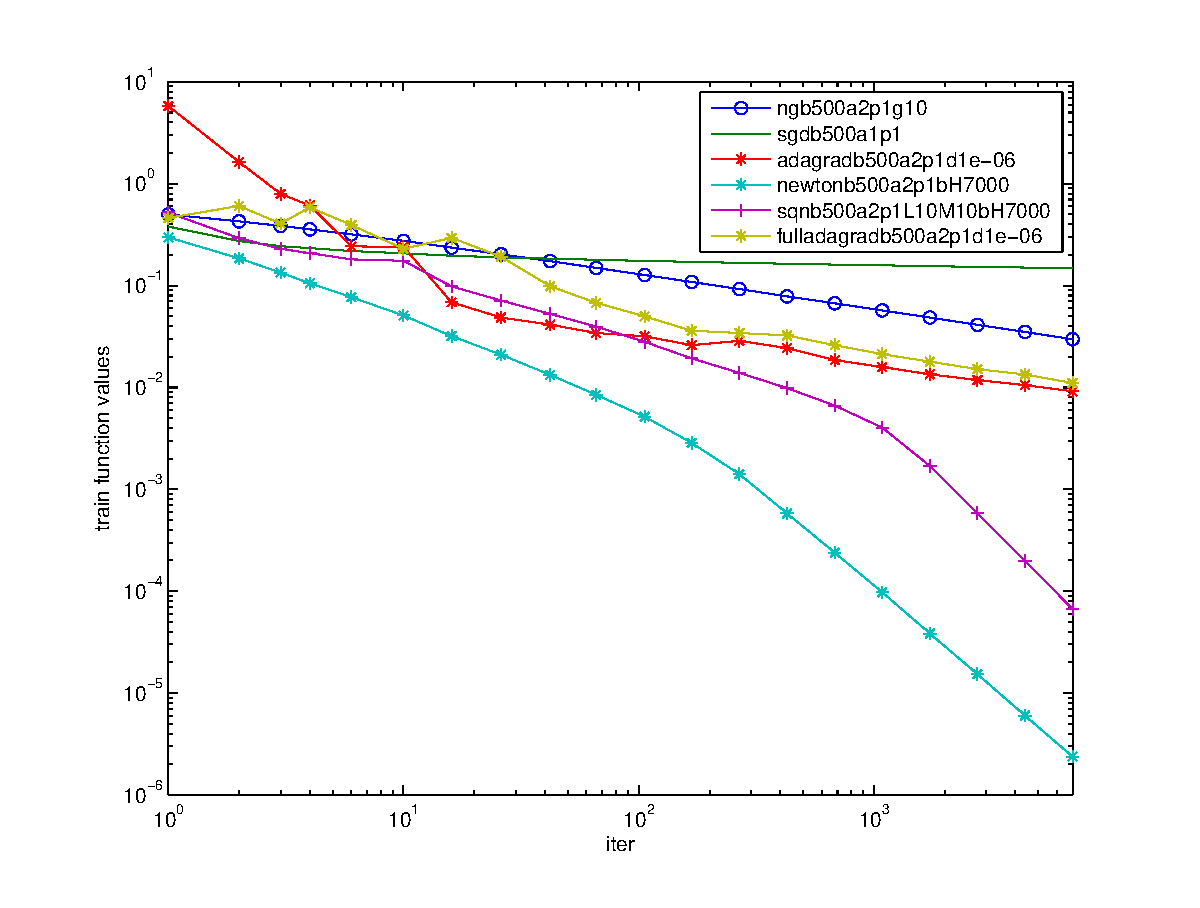
\includegraphics[scale=1]{paperOnImpFigures/yoram-train-6.eps}
\subsubsection{test}
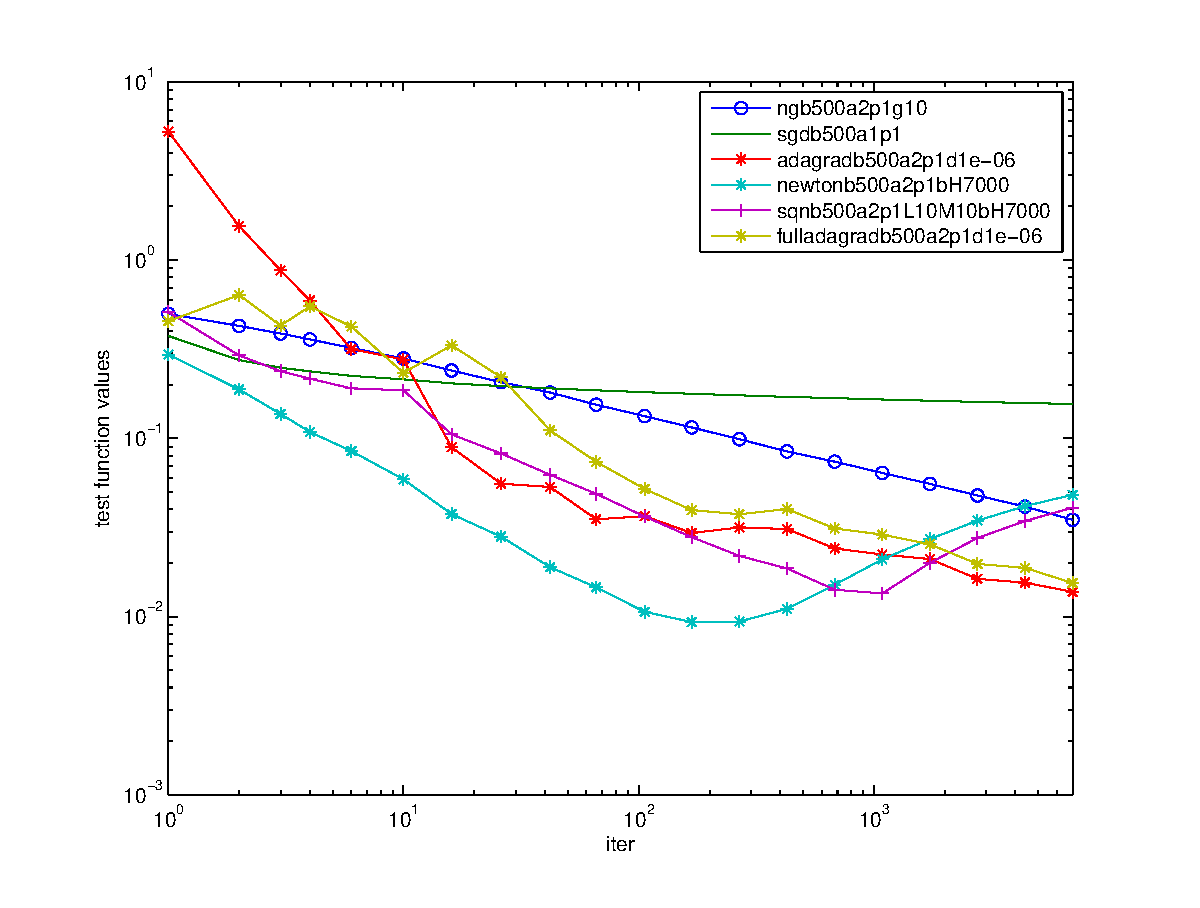
\includegraphics[scale=1]{paperOnImpFigures/yoram-test-6.eps}
\subsubsection{Questions}

Tune based on testing or training error? \\
Tune based on how many passes over data? \\

\subsection{Amari's Natural Gradient}
Let $S = \{ w \in \mathbb{R}^n \}$ be a parameter space on which $L(w)$, the loss function is defined. For $S$ Euclidean, 
\begin{equation}
	\|dw\|^2 = \sum (dw_i)^2
\end{equation}
Otherwise,
\begin{equation}
	\|dw\|^2 = \sum g_{ij}dw_i dw_j
\end{equation}
The parameter space in neural networks has the Riemannian character.
Steepest descent is $dw$ taht minimizes $L(w+dw)$ for a fixed length $\phi$.
In a Riemannian space, 
\begin{equation}
	\tilde{\nabla L(w)} = \nabla L(w) G^{-1} \nabla L(w)
 \end{equation}
Where $G = (g_{ij})$. Amari claims that the Riemannian structure of the parameter space of a statistical model is defined by the Fisher Information. 
For a statistical model, 
\begin{equation}
	g_{ij}(w) = E \left[ \frac{\partial \log p(x,w)}{\partial w_i} \frac{\partial \log p(x,w)}{\partial w_j} \right]
\end{equation}
For a multilayer network, 
\begin{equation}
	g_{ij}(w) = E \left[ \frac{\partial \log p(x,y;w)}{\partial w_i} \frac{\partial \log p(x,y;w)}{\partial w_j} \right]
\end{equation}
Yann Olivier likes this, and develops four methods using the natural gradient. He claims that Second-order effects are emulated in the same way the Gauss–Newton algorithm emulates the Newton method.

\subsubsection{Takio Kurita Paper - 1994}
For a network with only one neuron, with a logistic output we have a model equivalent to Yoram's problem. The Fisher information is computed as the minus of the expected value of the Hessian. It can be thought as a weighted covariance of the input vectors. Fisher information is same as Hessian except the sign. This corresponds to the expression given in Yoshua Bengio's paper. 

For a network with one hidden layer, Fisher information is given as a weighted covariance matrix of inputs and outputs of hidden units. 


\subsubsection{Schraudolph}
$N$ is the network. $M$ is identity for linear outputs. $L$ is loss. 
Gradient is 
\begin{equation}
	g=J_N J_M J_L
\end{equation}
Extended Gauss-Newton matrix comes from ignoring the second term in 
\begin{equation}
	H = \frac{\partial}{\partial w} (J_{LoM} J_N)  = J_N H_{LoM} J_N + \sum_i (J_{LoM}) H_{N_i}
\end{equation}
Only second order interactions among N's outputs are modeled. This is a compromise between hessian which models all second order information and Fisher information which ignores it all. 

For linear outpus with sum-squared loss (conventional Gauss-Newton), $H_{LoM}  = J_M = I$. For logisitc outputs with cross-entropy loss it is $diag(diag(z)(1-z))$.


\subsubsection{Yoshua Bengio Paper}
The Natural Gradient algorithm steps in the direction
\begin{equation}
\nabla_N L(\theta) = \nabla L(\theta) E_z \left[ (\nabla \log p_{\theta}(z))^T  (\nabla \log p_{\theta}(z)) \right]^{-1}
\end{equation}
where $p$ is the distribution of features, and the gradients are taken with respect to $\theta$. $L$ is the loss function parametrized by $\theta$.
These can be computed precisely for the randomly generated problems generated with Yoram's scheme. 
   
  

\subsection{Efficient Approximations}
Here we test some known efficient approximations to the methods above.

\subsubsection{AdaGrad}
We code a diagonal AdaGrad version

\begin{algorithm}[H]
\caption{AdaGrad}
\label{alg1}
\begin{algorithmic}[1]
\REQUIRE  $\eta>0$ $\delta \geq 0$
\STATE  $t=0$ $s_{-1}=0$
\WHILE{$x^t$ doesn't satisfy stopping condition}   
\STATE $s_{t,i} = \frac{1}{t} \sqrt{   \sum_{j=1}^t g_{j,i}^2   }  =\frac{1}{t} \sqrt{ ((t-1) s_{t-1,i})^2 +g_{t,i}^2 }  $
\STATE $H_t = \frac{\delta I}{t} + diag(s_t)$
\STATE $x^{t+1} = x^t - \frac{\eta}{t} H_t^{-1} g_t$
\STATE $t=t+1$
\ENDWHILE
\end{algorithmic}
\end{algorithm}

There is no need to store the actual history $1:t$. The update to $s_t$ can be done recursively. 

Need to tune the constant steplength $\eta$. In practice $\delta$ can be set to 0

Quote from AdaGrad there is no need to keep track of a learning rate as in previous algorithms, as it is imlicitly given by the growth of the proximal function

\begin{itemize}
	\item Using a leaky average of the per-example Gauss-Newton approximation of the Hessian (Bottou, Le Cun. Large Scale Online Learning 2004)
	\item Diagonal Adagrad version
	\item Stochastic Quasi-Newton methods
\end{itemize}

\subsection{Neural Nets}
Here the Gauss-Newton case is more interesting due to the fact that there are multiple layers, and it is not equivalent to the Hessian matrix. 


\section{SQN vs AdaGrad}

I have intentionally left the p1 in the labels - this is meant to signify that I used $\alpha/k$ for the steplength strategy. This is useful to distinguish from any constant step tests. I tried different powers of 2 for the AdaGrad experiments. All plots below show progress for running for work equivalent to five passes through the data. 

\subsection{Yoram}

\subsubsection{train}
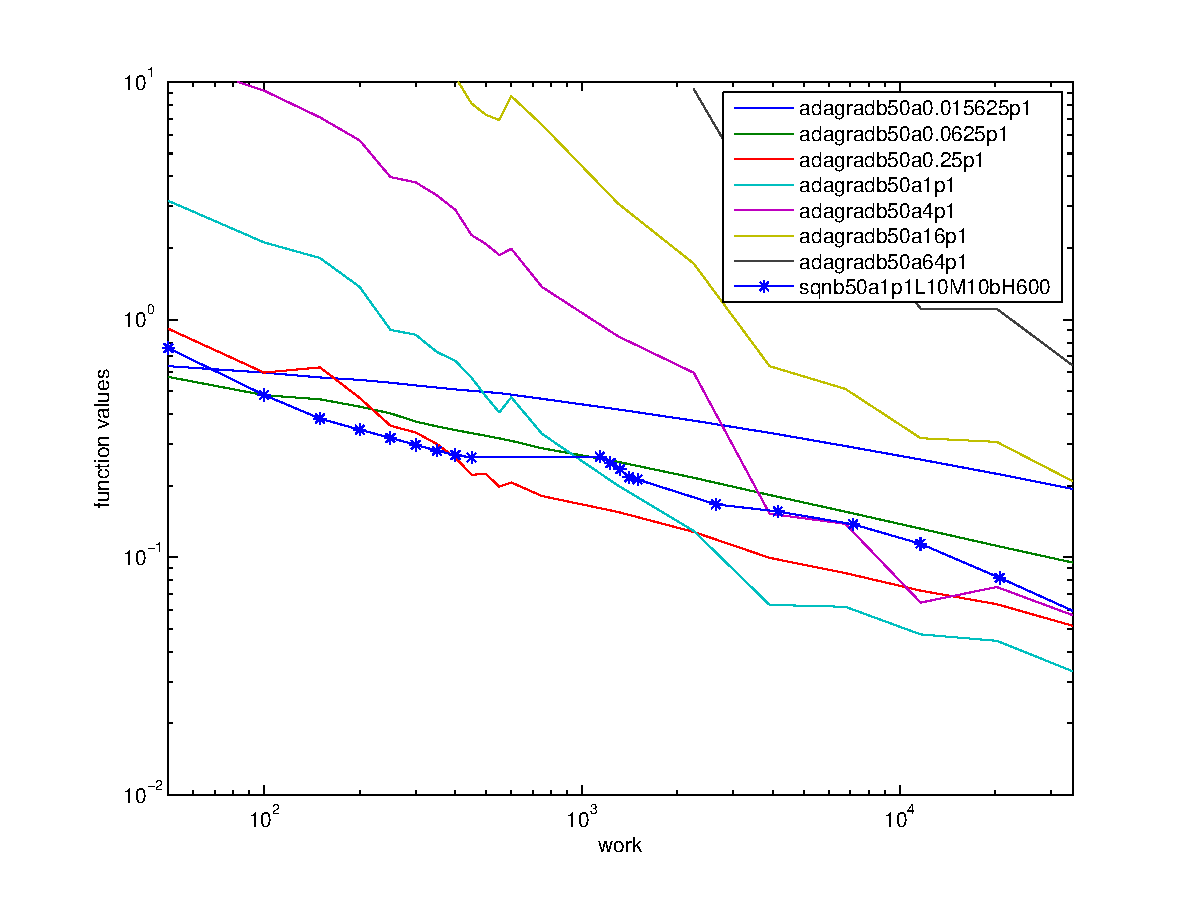
\includegraphics[scale=1]{paperOnImpFigures/yoram-adagrad-l-train.eps}

\subsubsection{test}
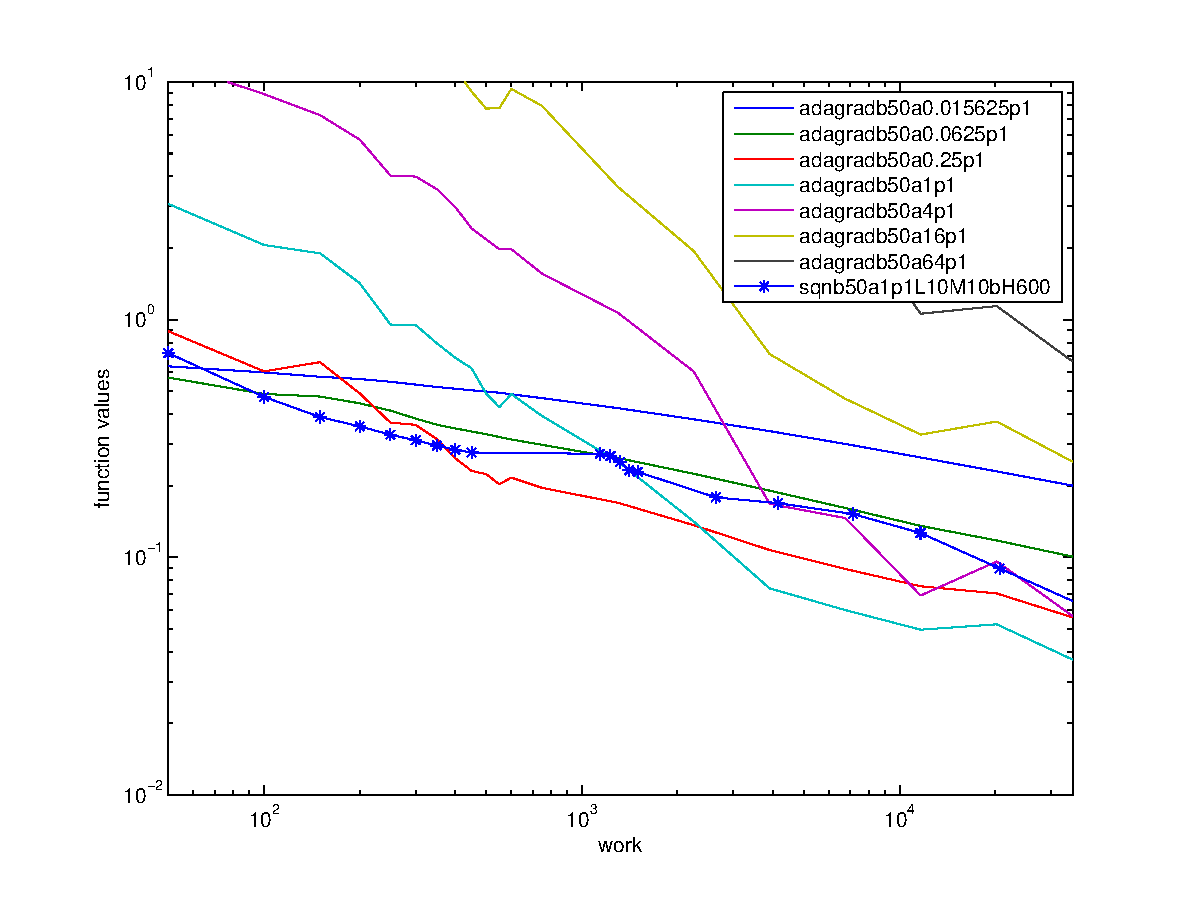
\includegraphics[scale=1]{paperOnImpFigures/yoram-adagrad-l-test.eps}

\subsection{Speech}

\subsubsection{train}
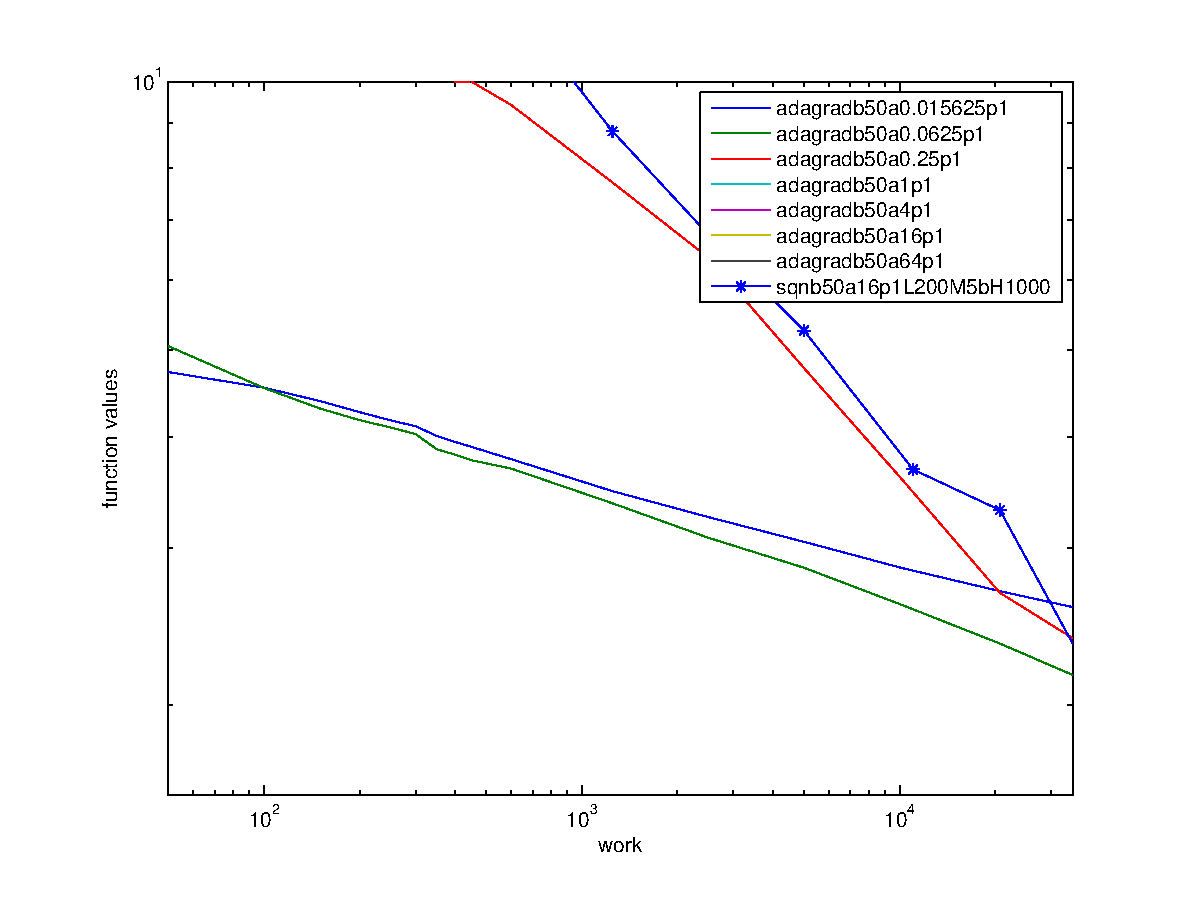
\includegraphics[scale=1]{paperOnImpFigures/speech-adagrad-l-train.eps}
\subsubsection{test}
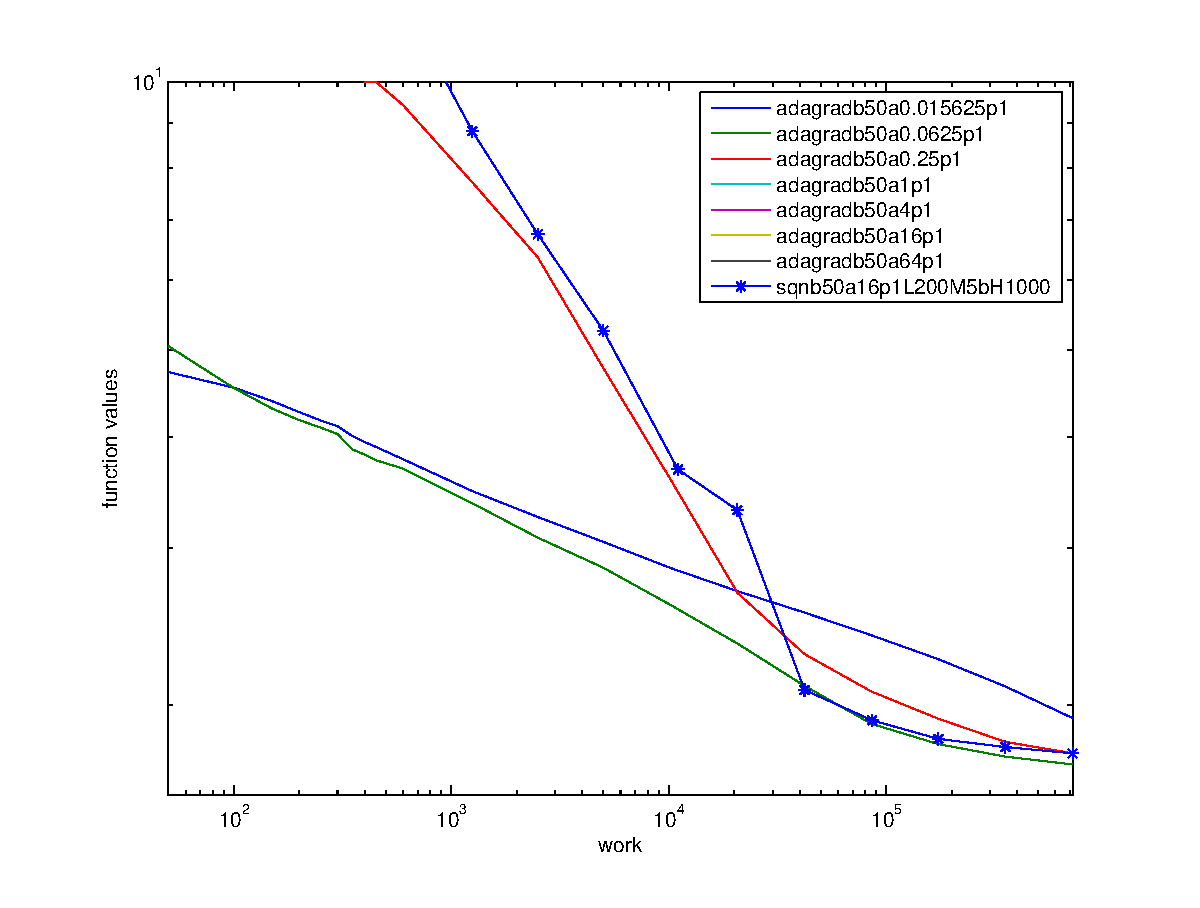
\includegraphics[scale=1]{paperOnImpFigures/speech-adagrad-l-test.eps}


\subsection{RCV1}

\subsubsection{train}
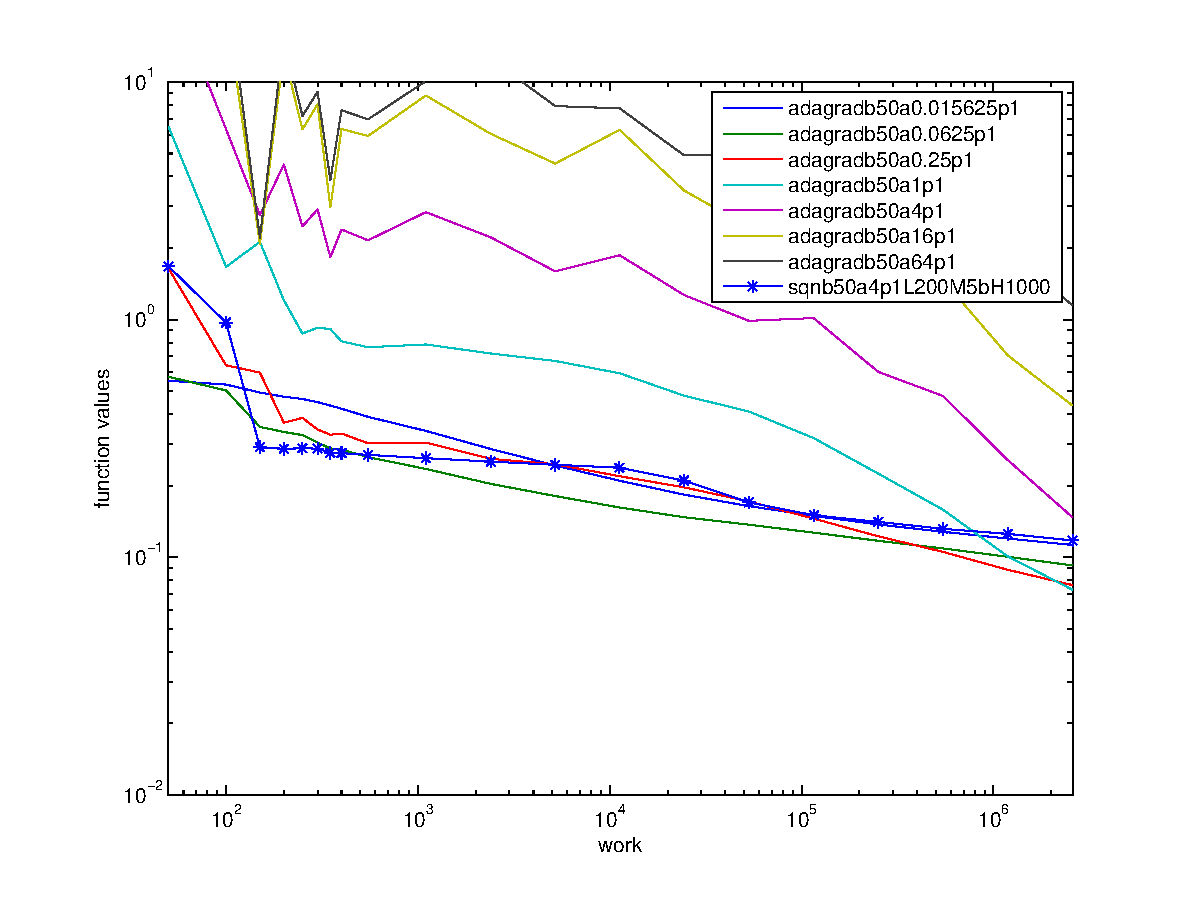
\includegraphics[scale=1]{paperOnImpFigures/rcv1-adagrad-l-train.eps}
\subsubsection{test}
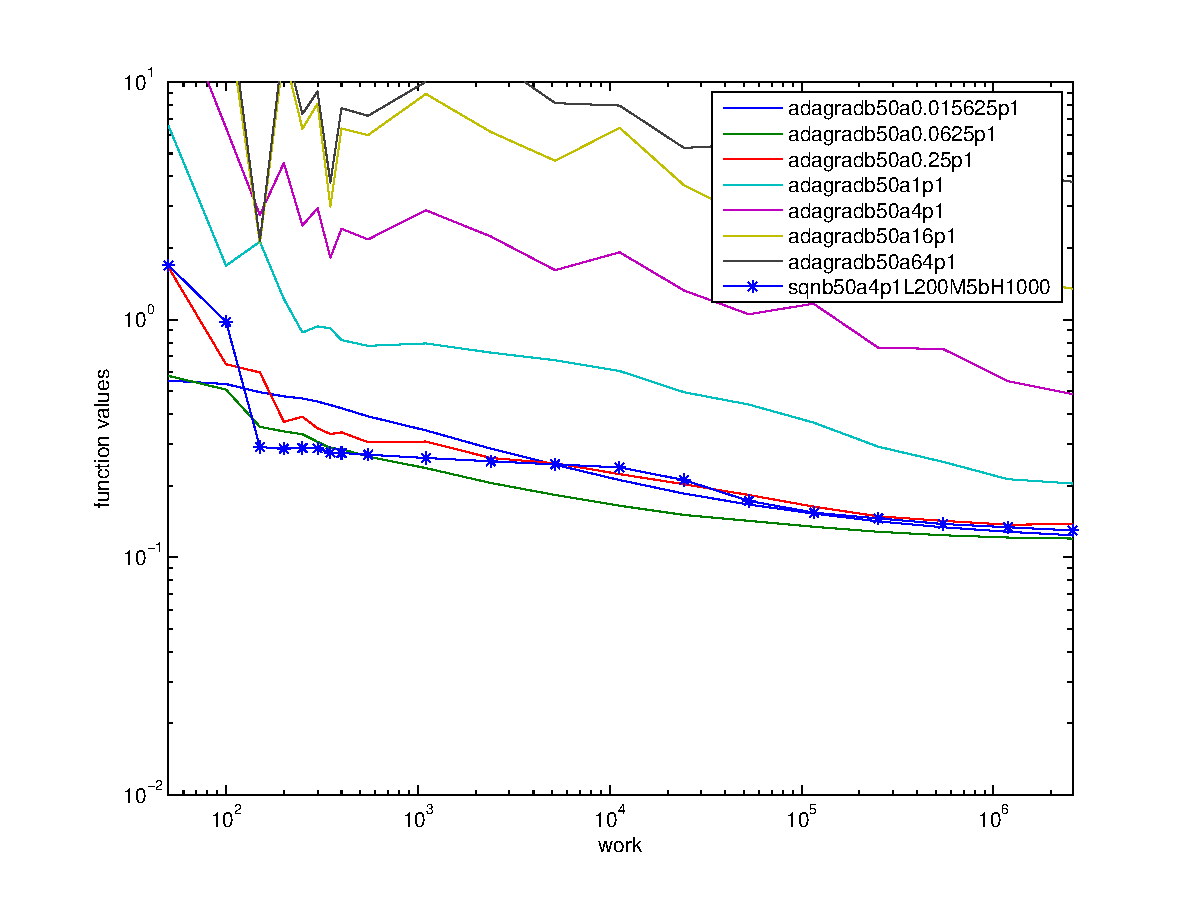
\includegraphics[scale=1]{paperOnImpFigures/rcv1-adagrad-l-test.eps}

\section{More experiments}


Test whether sqn will work without 
\begin{verbatim}
    if norm(s) > 1
        s = s/norm(s);
    end
\end{verbatim}

Test whether a fast generalization error will actually work for Yoram's problem.

\section{Experiment with using gradient differencing with consistent samples}

In equation (2.3) in the stochBFGS, we will use the consistent batches. This is an alternative approach to using the hessian-vector product, and is another tool to ensure consistency. 

\end{document} 
